\RequirePackage[l2tabu,orthodox]{nag}
%
\documentclass[oneside,a4paper,oldfontcommands]{memoir}

%\newsubfloat{figure}

\PassOptionsToPackage{table,svgnames,dvipsnames}{xcolor}

\usepackage{MyriadPro}
\usepackage{MinionPro}
\usepackage[scaled]{beramono}
%\usepackage{lmodern}
\usepackage[utf8]{inputenc}
% \usepackage[sc]{mathpazo}
\usepackage[T1]{fontenc}
%\usepackage{tgpagella}
%\linespread{1.05}
\usepackage[english]{babel}
\usepackage{syntax}
\usepackage{subcaption}
\usepackage[lang=en,grid]{kufront}
% \usepackage[american]{babel}
\usepackage[autostyle]{csquotes}
\usepackage[acronym]{glossaries}
\usepackage{todonotes}
\usepackage{fancyvrb}
%\usepackage{adjustbox}

% \newminted{c}{fontsize=\small}


\usepackage[super]{nth}
\usepackage{xcolor}

% \nth{1}, \nth{2}, \nth{3}, \nth{4}

\usepackage{multicol}

% \newenvironment{blocklisting}[1]
% {\begingroup\lstset{#1}\VerbatimOut{blocklisting-tmp.txt}}
% {\endVerbatimOut\begin{block}{Code}\lstinputlisting{blocklisting-tmp.txt}\end{block}\endgroup}
\newenvironment{smeilcode2}
{\begingroup\lstset{language=smeil}\VerbatimOut{blocklisting-tmp.txt}}
{\endVerbatimOut\begin{multicols}{2}\lstinputlisting{blocklisting-tmp.txt}\end{multicols}\endgroup}

%\renewcommand{\ttdefault}{cmtt}
\newcommand{\libsme}[0]{\textsc{libsme}}

\newcommand{\codemargins}[0]{\paperwidth-2cm}

\newenvironment{widefigure}[1][]{
  \begin{figure}[#1]
  \centerfloat
  \begin{minipage}[t]{\codemargins}
  }{\end{minipage}
   \end{figure}
}

% Define some colors
\definecolor{mblue}{RGB}{0,0,200}
\definecolor{mred}{RGB}{200,40,0}
\definecolor{mgreen}{RGB}{0,180,0}
\definecolor{mdarkgreen}{RGB}{0,100,0}
\definecolor{morange}{RGB}{200,100,0}

\definecolor{lightblue}{RGB}{197,227,240}
\definecolor{lightgreen}{RGB}{197,240,184}

\definecolor{scopebg}{RGB}{250,250,250}
\definecolor{scopeborder}{RGB}{200,200,200}

\usetikzlibrary{calc}
\usetikzlibrary{positioning}
\usetikzlibrary{arrows.meta}
\usetikzlibrary{shapes}
\usetikzlibrary{matrix}
\usetikzlibrary{fit}
\usetikzlibrary{patterns}
\usetikzlibrary{backgrounds}
\usetikzlibrary{decorations.pathreplacing}


% \usepackage[utf8]{inputenc}
% \usepackage[T1]{fontenc}
%\usepackage[danish,english]{babel}
%\usepackage{urw-garamond}


  %url=false,
  %style=alphabetic,
  %citestyle=authoryear-icomp,
\usepackage[%
  backend=biber,
  style=numeric,
  maxnames=2,
  minnames=1,
  maxbibnames=99,
  firstinits,
  uniquename=init,
  backref=true]{biblatex} % TODO: adapt citation style
  %maxcitenames=2,

\AtEveryBibitem{%
  \ifentrytype{onlinex}{%
  }{%
    \clearfield{url}%
    \clearfield{urldate}%
  }%
}

% \usepackage{graphicx}
% % \usepackage{listings}

% \usepackage{minted}
\usepackage{diagbox}
\usepackage{lstautogobble}
\usepackage{tikz}
%\usepackage{pgfplots}
%\usepackage{pgfplotstable}
\usepackage[margin=1cm,font=small,labelfont=bf]{caption}
%\captionnamefont{\bfseries}


\usepackage{booktabs}
%\usepackage[final]{microtype}
\usepackage[draft]{fixme}
\usepackage{wrapfig}
%\usepackage{caption}
%\usepackage[inline]{enumitem}
%\setlist[enumerate,1]{label=\textit{\alph*)}}
\usepackage{paralist}
\usepackage[hidelinks]{hyperref} % hidelinks removes colored boxes around references and links
\usepackage[euler]{textgreek}
\usepackage[nameinlink]{cleveref}
%\usepackage{refcheck}
%\usepackage{scrhack} % necessary for listings package

%%% Infrastructure    
% \makeatletter
% \newcommand{\refcheckize}[1]{%
%   \expandafter\let\csname @@\string#1\endcsname#1%
%   \expandafter\DeclareRobustCommand\csname relax\string#1\endcsname[1]{%
%     \csname @@\string#1\endcsname{##1}\wrtusdrf{##1}}%
%   \expandafter\let\expandafter#1\csname relax\string#1\endcsname
% }
% \makeatother
%%%

%%% Now we add the reference commands we want refcheck to be aware of
% \refcheckize{\cref}
% \refcheckize{\Cref}

%\addtokomafont{caption}{\small}
%\setkomafont{captionlabel}{\sffamily\bfseries}

\bibliography{bibliography}

%\setkomafont{disposition}{\normalfont\bfseries} % use serif font for headings
%\setkomafont{disposition}{\sffamily} % use serif font for headings
%\linespread{1.05} % adjust line spread for mathpazo font

% Add table of contents to PDF bookmarks
%\BeforeTOCHead[toc]{{\cleardoublepage\pdfbookmark[0]{\contentsname}{toc}}}

% Settings for pgfplots
% \pgfplotsset{compat=newest}
% \pgfplotsset{
%   % For available color names, see http://www.latextemplates.com/svgnames-colors
%   cycle list={CornflowerBlue\\Dandelion\\ForestGreen\\BrickRed\\},
% }

% Settings for lstlistings
% \lstset{%
%   basicstyle=\ttfamily,
%   columns=fullflexible,
%   autogobble,
%   keywordstyle=\bfseries\color{MediumBlue},
%   stringstyle=\color{DarkGreen}
% }

\lstdefinelanguage{smeil}
{
  morekeywords={
    as,
    assert,
    async,
    barrier,
    break,
    bus,
    case,
    const,
    default,
    elif,
    else,
    enum,
    exposed,
    for,
    from,
    func,
    generate,
    if,
    import,
    in,
    instance,
    network,
    of,
    out,
    proc,
    range,
    return,
    simulation,
    switch,
    sync,
    to,
    trace,
    unique,
    var
  },
  sensitive=true,
  morecomment=[l]{//},
  morestring=[b]''
}
\lstset{
  columns=fixed,
  %basicstyle=\ttfamily\bfseries\small,
  basicstyle=\small\fontfamily{pcr}\selectfont,
  emphstyle=,
  %keywordstyle=,
  numbers=none,
  firstnumber=auto,
  identifierstyle=,
  commentstyle=,
  stringstyle=,
  showstringspaces=false,
  captionpos=b,
  xleftmargin=16pt,
  escapeinside={??}
}
\lstnewenvironment{smeilcode}{\lstset{language=smeil}}{}
\lstnewenvironment{pythoncode}{\lstset{language=python}}{}

%%% Local Variables:
%%% mode: latex
%%% TeX-master: "master"
%%% TeX-command-extra-options: "-enable-write18"
%%% End:


\newacronym{sme}{SME}{Synchronous Message Exchange}
\newacronym{csp}{CSP}{Communicating Sequential Processes}
\newacronym{gpl}{GPL}{General Purpose Language}
\newacronym{dsl}{DSL}{Domain-specific Language}
\newacronym{vhdl}{VHDL}{VHSIC Hardware Description Language}
\newacronym{hdl}{HDL}{Hardware Description Language}
\newacronym{smeil}{SMEIL}{SME Implementation Language}
\newacronym{vhpi}{VHPI}{VHDL Prodecural Interface}
\newacronym{sloc}{SLOC}{Source Lines Of Code}
\newacronym{il}{IL}{Intermediate Language}
\newacronym{axi}{AXI}{Advanced eXtensible Interface}
\newacronym{hls}{HLS}{High-Level Synthesis}
\newacronym{csv}{CSV}{Comma-Separated Values}
\newacronym{gpgpu}{GPGPU}{General Purpose Graphics Processing Unit}
\newacronym{cpu}{CPU}{Central Processing Unit}
\newacronym{fpga}{FPGA}{Field-Programmable Gate Array}
\newacronym{ic}{IC}{Integrated Circuit}
\newacronym{asic}{ASIC}{Application Specific Integrated Circuits}

%%% Local Variables:
%%% mode: latex
%%% TeX-master: "../master"
%%% TeX-command-extra-options: "-enable-write18"
%%% End:

\makeglossaries

%\headstyles{ell}
\chapterstyle{ell}

% Use sans-serif font
\renewcommand{\kufrontfont}{\sffamily}

\project{\mdseries\LARGE Master's Thesis}
\author{Truls Asheim --- {\ttfamily truls@asheim.dk}}
%\title{A Common Intermediate Representation of Synchronous Message ExchangeNetworks}
%\title{This is a title}
\title{A Domain Specific Language for Synchronous Message Exchange Networks}
%\subtitle{ }
\date{May 2018}
\supervisor{Supervisors: Brian Vinter and Kenneth Skovhede}

\begin{document}

\frontmatter

\begin{titlingpage}
\maketitle
\end{titlingpage}

\newpage
%\pagestyle{plain}
\begin{abstract}
  Synchronous Message Exchange (SME) is a Concurrent Sequential Processes
  (CSP)-derived model for hardware designs implementing globally synchronous
  message passing. SME implementations currently exist for several
  general-purpose languages, some of which, are translatable to VHDL for
  subsequent implementation on hardware. A common SME language could reduce the
  duplication and feature disparity present in these independent
  implementations. This thesis introduces a domain-specific language for
  implementing SME designs. It is usable both as a primary implementation
  language for SME models and as an intermediate target for general-purpose
  languages. We describe the language, its implementation and its
  features. Furthermore, we explain the specific requirements for a language
  within this domain. Finally, we evaluate the language through a number of
  simple, but realistic, hardware designs by showing how they may be implemented
  and tested.
\end{abstract}
\newpage


\newpage
\tableofcontents

\printglossary[type=\acronymtype,title=Abbrevations]

% \chapter{Preface}
% This thesis is submitted in fulfillment of the degree {\it Master of Computer
%   Science} for Truls Asheim.

% \chapter{Acknowledgements}
% First of all, I would like to extend my gratitude towards Brian Vinter and
% Kenneth Skovhede for this, and previous, highly interesting projects that I
% have carried out under their supervision. I would also like to thank the
% eScience group at the Niels Bohr Institute for providing a highly welcoming
% environment. In particular by offering myself, and the other Master's Thesis
% students, office space and inviting us along to the strategy retreat. It was
% highly appreciated! For taking their time to read my thesis and providing
% insightful comments I would like to thank my lovely proofreaders: Last but not
% least

\mainmatter

\chapter{Introduction}

Special-purpose hardware has a wide range of different uses and can provide a
significantly improved performance-to-watt ratio compared to GPGPUs and CPUs for
many applications. Unfortunately, the prevalence of such hardware is limited, in
part, by poor design tools. Traditional hardware design workflows utilize
{\itshape Hardware Description Languages} (HDLs) such as \gls{vhdl} or Verilog
which require the programmer to specify the hardware design at a very low
level. While this enables complete control over the resulting hardware, the
productivity sacrifice is significant when compared to using general-purpose
languages for writing software. Additionally, all aspects of a hardware design
are often written in a HDL, including code for testing and
verification. Traditional HDLs are fundamentally unfit for performing tasks
commonly needed for simulating input for a design, such as reading and decoding
an image file. Performing them are tedious at best and impossible at worst.

In the past few decades, there has been a significant interest in tools that
improve the productivity of hardware design workflows. Vendors of reconfigurable
hardware have focused primarily on {\itshape High-Level Synthesis} (HLS). These
utilities transform algorithmic descriptions written in a general-purpose
language to an HDL-description that can be implemented on hardware. The source
languages for the most common HLS tools are C (e.g. Vivado HLS~\cite{vivadohls})
and OpenCL (e.g. Altera OpenCL~\cite{aocl}).

Hardware is inherently parallel, and utilizing this parallelism is imperative
for achieving good performance. Therefore, efficiently transforming sequential C
code to a hardware description requires inferring parallelism in a similar
manner to, for example, OpenMP. To control the transformation, the programmer is
required to add annotations to the C program. The quality and performance of the
resulting hardware implementation depend greatly on the aptitude of the
programmer to add these annotations correctly. This requires a deep
understanding of the transformation process and the underlying architecture of
the targeted hardware. The difficulties of creating auto-parallelizing compilers
for impure general-purpose languages are
well-known~\cite{banerjee1976data,bodik2000abcd} in particular due to the
challenges of resolving data dependencies. HLS utilities provide no
revolutionary improvements in this regard and thus have a tendency to retain
major sequential parts of the original program causing an inefficient hardware
design.

Transforming OpenCL programs to hardware descriptions is a related scheme which
is currently gaining popularity. This option seems more attractive as OpenCL is
already an explicitly parallel language targeting heterogeneous computing
platforms. However, OpenCL code needs to be tuned specifically to each target
platform in order to achieve optimal performance~\cite{chen2012using}. Most
existing OpenCL programs are written with GPGPUs in mind. Thus, these programs
must be rewritten to perform optimally on FPGAs, again requiring heavy use of
annotations. This reduces the portability and productivity advantages of OpenCL.
% Furthermore, OpenCL is most efficient when
% applied to problems which exhibit a high-degree of data parallelism, but
% problems exhibiting other kinds of concurrency are more difficult to
% model.\todo{Is this right?}.
Furthermore, the OpenCL computing model requires the presence of a host device
which makes it unsuitable for creating completely independent hardware
components.

To approach this problem from a different angle, the Synchronous Message
Exchange (SME) model\cite{vinter2015bus,vinter2014synchronous} has been
previously introduced. SME is similar to \gls{csp}~\cite{csp}, but replaces the
asynchronous communication of CSP with globally synchronous message passing
between processes driven by a hidden clock\footnote{An extended introduction to
  the SME model is given in \Cref{sec:sme}}.
% This communication model mimics hardware where all signal propagations
% are also globally synchronous, driven by a clock.
This allows the programmer to be explicit about concurrency, using a model which
closely resembles signal propagation in hardware. Thus, SME simplifies
performance reasoning compared to the HLS approaches described above.

As the implementations of SME has advanced, it has been utilized to create
several successful hardware designs which have been implemented on FPGAs. For
example, a MIPS processor implemented in SME was successfully synthesized and
implemented on an FPGA~\cite{johnsen2017thesis}. These achievements have
motivated and encouraged the continuing development of the model and related
utilities, although we do not claim that it has reached the level of maturity of
the HLS approaches previously mentioned.

SME by itself is just a model, which is not tied to a specific programming
language or implementation. Currently, libraries for implementing SME models
exist for the general-purpose languages C++~\cite{asheim2015},
C\#~\cite{skovhede2016building} and Python~\cite{asheim2016vhdl}. The latter two
have code-generation backends targeting VHDL. In practice, it has proven
impossible to maintain feature parity between these independent implementations
due to the code-duplication involved. This created a demand to unify the common
backend components of these divergent code bases. To achieve this, a common
intermediate language for SME networks was needed. While we could feasibly
introduce an interface allowing this between Python and C\#, the number of
required interfaces increase exponentially for every language added. Having a
common intermediate language would make this integration simple. Furthermore,
combining SME networks written in different source languages was also a desired
feature.

This thesis introduces the SME Implementation Language (SMEIL, pron. ``smile'')
and its accompanying implementation, \libsme{}~\cite{libsme}.
% SMEIL is an attempt to provide the best of both worlds
% by separating the actual hardware description and assigning them to the best
% suited languages.
SMEIL is a specialized language, featuring a familiar C-like syntax and
structural constructs which are deeply rooted in the SME model. Furthermore, it
provides a type-system which is tailored for hardware-specific subtleties that
are difficult to express in general-purpose languages without deviating from
established paradigms. An explicit design goal of SMEIL is to allow a simple and
straight-forward mapping of code structures commonly found in imperative
general-purpose languages.  For testing designs implemented in SMEIL,
general-purpose languages are well suited since their full range of available
libraries can be utilized. \libsme{} provides a simple, language-independent,
API allowing SME implementations written for general-purpose languages to
communicate with SME networks written in SMEIL.

Although SMEIL was initially intended purely as an intermediate language target
for existing SME implementations, the resulting language has additionally proven
to be usable as an independent primary implementation language for SME
models. The remainder of the thesis will primarily describe the language from
this perspective. To show its use as an intermediate language, we have adapted
our previous implementation of a Python SME to VHDL compiler~\cite{almique} to
output SMEIL instead of VHDL directly. This is discussed in \Cref{sec:smeilil}.


\section{Motivations for a SME DSL}
\label{sec:smemot}

Initially, we considered just creating a common Abstract Syntax Tree (AST)
representation. This approach would focus on generalizing the existing ASTs
already used internally by the PySME and C\# SME to VHDL transformers. An
advantage of this strategy is that it carries a smaller implementational burden
compared to creating a dedicated language. However, no simple and established
frameworks exist for formally specifying an AST in a language-neutral way. A
representation without a corresponding concrete syntax would also be difficult
to understand and reason about, making it hard to verify the correctness of the
generated intermediate code.

At this point, the language had a concrete syntax of its own and fulfilled the
original design goal of providing a direct mapping of constructs from common
general-purpose languages. The reason for this design goal was to ensure that
adding new SME frontends would be as simple as possible, relieving them of
having to perform sophisticated transformations. Thus, SMEIL inevitably became
an independent DSL suitable as a primary implementation language for SME
models. Exploring the concept of an independent SME DSL is interesting for a
number of reasons. In particular, A DSL allows concise and elegant expression of
concepts present in the target domain---the domain-specific needs of hardware
are not considered in the design of general-purpose software languages.

\paragraph{C\# SME.}
Translating SME models written in C\# is comparatively straight-forward since
language properties can be statically specified and are enforced by the
compiler. For example, if we declare a variable as being constant, we can be
sure that its value will never change beyond its initial assignment and
fixed-length arrays may be explicitly created as such. Likewise, when we declare
a variable to be of a certain type, we can be sure that it will keep that type
throughout the program. Being able to specify such restrictions is immensely
useful as the transformation target (a hardware description), is also
static. However, this also means that hardware-targeted SME models written in
C\# contains a lot of declarational ``noise'' required to confine the C\#
language to a feature set which is possible to implement on hardware. Since the
C\# syntax cannot be extended to natively declare SME elements, annotations are
required to inform the SME runtime and translation system about how a C\# object
should be interpreted.


\paragraph{PySME.}
The situation is different for languages such as Python. The key selling point
of Python is that it is a high-productivity language which is simple to use. It
largely owes these attributes to the fact that it is a dynamic
language. However, this makes it challenging to determine the static properties
needed in a hardware description from a Python program without imposing a heavy
annotational burden. Furthermore, building upon our C\# example from before,
ensuring that a Python variable retains its type throughout program execution
require either sophisticated analyses or strong programmer discipline. Being
able to provide such guarantees is a prerequisite for performing a semantically
unchanged transformation. We base these assertions on our previous experience
building a Python SME to VHDL compiler~\cite{asheim2016vhdl}. While we were able
to transform SME networks written in Python to VHDL, the programmer could only
use a narrow and strictly specified subset of Python in the hardware-targeted
processes. The addition of unfamiliar features (annotations), and required
re-learning of semantic assumptions, reduces the advantage of Python from the
perspective of an experienced Python programmer. It is certainly possible to
improve on our previous attempt at transforming Python. However, this is a
significant effort which does not directly contribute to the capabilities of SME
as a hardware design utility.

% An extreme example of why Python is not always a good ideas is SysPy which uses
% python in a way that almost word-for-word mirrors VHDL and its idiosyncrasies;
% this is exactly what SME is trying to avoid!

% To summarize these assessments, our underlying conjecture is that the underlying 
\vspace{1em} The key advantage of writing SME models in a general-purpose
language is that test-benches can utilize the full range of libraries available
for that language. It is crucial that this advantage is preserved for SME
networks written in SMEIL. We explain how this is achieved in
\Cref{sec:cosim}. A common objection towards DSLs is the requirement of learning
a new and unfamiliar language. However, the SME model itself needs to be learned
in any case and the additional overhead SMEIL imposes is minimal. From
first-hand experience, a student of computer science familiar with CSP, but not
SME, was able to start writing simple SMEIL programs after just a few hours of
introduction.

Due to its origins as an intermediate language, its syntax is not the
friendliest in the world. The syntax attempted to strike a balance between being
simple to parse while not being completely unreadable for humans.

\section{Limitations}
This thesis does not discuss the low-level details of hardware design beyond a
brief introduction to hardware design workflows. As previously mentioned, the
feasibility of SME as a hardware design tool has already been established
through previous successful implementations. All of our references to hardware
design are based on these previous experiences. The problems addressed in this
thesis are purely related to the SME model and the results of our work does not
alter the {\itshape fundamental} qualities of SME as a hardware design tool.


\section{Contributions}
We summarize the contributions of the thesis as follows

\begin{itemize}
\item We present a new language for implementing SME networks. The language is
  suitable both as a primary implementation language for SME networks and as an
  intermediate language for other SME implementations.
\item We provide a way to test models written in the language using a
  co-simulation approach.
\item We provide a method for deriving the minimally required bit-widths of
  wires in the final design from the observed range of values assigned to them
  during simulation.
\item We demonstrate an implementation of the above points in addition to VHDL
  code generation from designs written in the introduced language.
\end{itemize}

\noindent A paper based on this thesis has been submitted for publication as

\begin{center}
\begin{minipage}{0.8\textwidth}
  T. Asheim, “SMEIL: A Domain Specific Language for Synchronous Message Exchange
  Networks”. In: {\itshape Proceedings of Communicating Process Architectures
    2018} (2018)
\end{minipage}
\end{center}

\section{Notation and Definitions}
We frequently refer to hardware-design nomenclature: A {\itshape test-bench} is a
piece of software used for testing a hardware model by providing input data and
verifying its output. {\itshape Synthesis} is the process of transforming a
hardware-model written in a HDL to an actual description which can be
implemented on hardware. We will occasionally refer to ``assigning a
value''. The ``value'' here may, unless specified otherwise, be any assignable
SMEIL construct (either a variable or a bus channel).

\section{Thesis Structure}
The remainder of the thesis is structured as follows.
\todo{finish}


% \section{Contributions}
% I summarize the contributions of this thesis as follows.

% \begin{itemize}
% \itshapeem I present a new Domain Specific Language, \gls{smeil}, which supports
%   implementing \gls{sme} networks. This language is suitable both as a primary
%   implementation language for \gls{sme} networks and as an intermediate language
%   which may be targeted by other implementations of \gls{sme}. This language can
%   be used as part of several design workflows. It may be used both in complete
%   isolation where the \gls{smeil} program alone produces a \gls{vhdl} hardware
%   description. It can also be used in conjunction with other languages.

% \itshapeem This language is presented in the context of the history of \gls{sme} and
%   we present its tradeoffs related to lessons learned and choices made by
%   previous \gls{sme} implementations.

% \itshapeem We show how networks written in \gls{smeil} can interface with \gls{sme}
%   frameworks written in general-purpose language, providing what we refer to as
%   co-simulation. By doing this, we mitigate the poor separation-of-concern
%   (described above) applying to both dedicated \gls{hdl}s and
%   \gls{gpl}'s. Through examples, we underpin the generality of this interface.

% \itshapeem We lay the building blocks for creating libraries of reusable \gls{sme}
%   components by presenting a module system for \gls{smeil}. In particular, we
%   establish the generality of \gls{smeil} by showing that such modules may be
%   combined regardless of the source language that produced the \gls{smeil}.

% \itshapeem We substantiate the feasibility of \gls{smeil} as an intermediate language
%   by showing that the high-level nature of \gls{smeil} easily supports
%   translation from and into several different languages.

% \itshapeem We argue for the advantages of using a \gls{dsl} over general-purpose languages
% by...

% \itshapeem As evidence, we supply a core compiler and simulator implementation,
%   written in Haskell, together with related library extensions to the PySME
%   library and Almique which embodies the qualities listed above. Furthermore,
%   C\# \gls{sme} was kindly extended by Kenneth Skovhede to support translation
%   to \gls{smeil}. The implementation is complete and functional and strives to
%   be of production quality. We spare the reader from further
%   implementation-specific details as these are often the least interesting parts
%   of a report like this. However, we refer to the supplied documentation for
%   details about how to use the supplied code.

% \itshapeem We show the suitability of the language for its intended purpose by
%   showing the simplicity of which a variety of different preexisting \gls{sme}
%   applications may be implemented in \gls{smeil}
% \end{itemize}



%%% Local Variables:
%%% mode: latex
%%% TeX-master: "../master"
%%% TeX-command-extra-options: "-enable-write18"
%%% End:

\chapter{Background}
\label{sec:sme}
In this chapter, we introduce the Synchronous Message Exchange (SME) model and
briefly describe its origins, evolution, semantics and implementations. The
design of SMEIL draws from the lessons learned throughout the, rather brief,
time period in which SME has existed. Here, we try to convey these insights to
the reader. Additionally, we further motivate the need for custom hardware.

\section{Synchronous Message Exchange}

\subsection{The Beginnings}
%The Synchronous Message Exchange model arose from a master thesis project 
The Synchronous Message Exchange model was conceived based on the experiences of
a masters thesis project \cite{Skaarup14} which attempted to generate a hardware
description from a model of a vector processor. The vector processor (described
in~\cite{rehr2013bpu}) was modeled with CSP using PyCSP, a CSP library for
Python. The initial experiences using CSP for modeling the processor were
promising. Especially the process abstraction of CSP proved to be well suited
for representing the discrete components of a hardware design. Furthermore, the
modularity originating from the {\itshape shared-nothing} property of CSP was
advantageous as it allowed seamlessly interchanging fine- and course grained
implementations of the same discrete component.

\begin{figure}
  \centering
  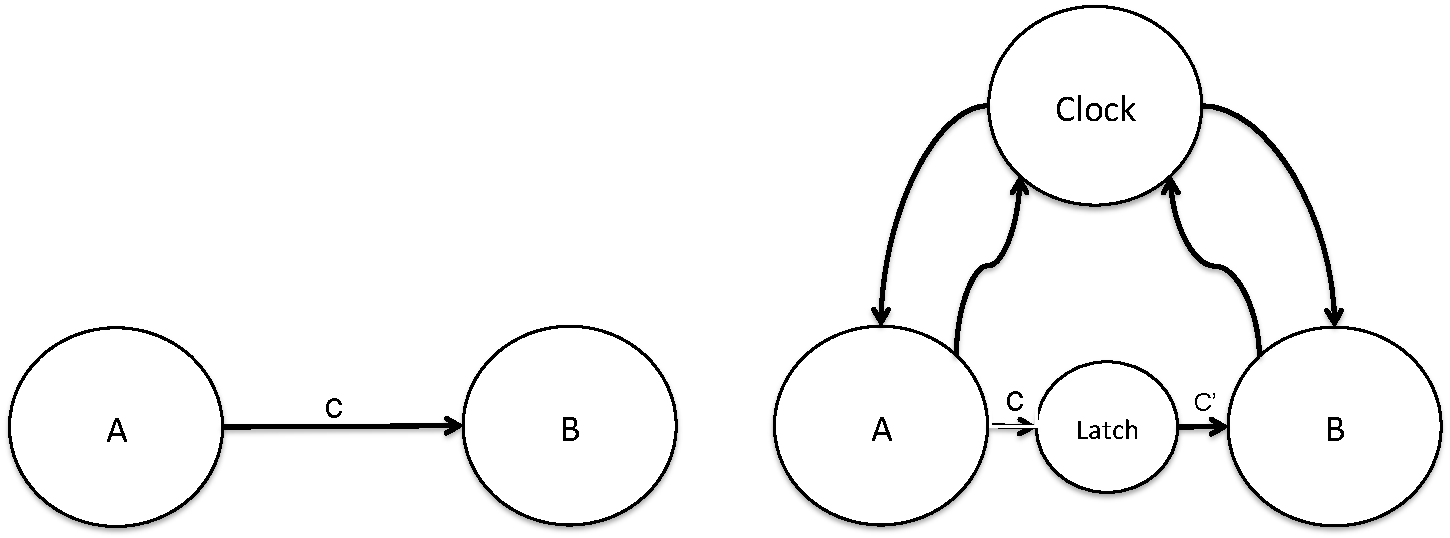
\includegraphics[width=0.9\textwidth]{figures/clocked.pdf}
  \caption{In order to enforce synchronous communication semantics on a simple
    CSP network, a large amount of additional complexity is needed. Figure
    from~\cite{vinter2014synchronous}.}
  \label{fig:clocked}
\end{figure}

When the master thesis project (mentioned above) later attempted to convert the pure
CSP model to a hardware description, they found the CSP approach less apt.
% which later attempted to convert
% the CSP model to an actual hardware description found the pure CSP approach less
% apt.
Their experiences revealed a fundamental discrepancy between the data
propagation models of hardware and of CSP. In CSP, a process is free to
communicate at any time while in digital hardware, all communication is driven
forward synchronously by a clock.
% Enforcing globally synchronous communication using CSP is hard, since
% CSP is inherently asynchronous.
Thus, to accurately model hardware using CSP, this clock had to be emulated by
adding a single clock process with broadcasting channels to every other process
in the network. Back-channels also had to be inserted for notifying
% from every process in the
% network to the clock process
the clock process when a process had finished running. Furthermore,
latch-processes had to be inserted into every channel going between processes,
ensuring that values were not propagated in the middle of a clock cycle. The
effect of adding these additional processes and channels is seen in
\Cref{fig:clocked}. Whenever the clock process emitted a signal, all processes
in the network would run. When the processes completed their run, the latch
processes ensured that values were propagated in the next cycle.
% When all processes had signaled a completed
% run, the clock would signal the latch processes in order to propagate the values
% of the network.

In the end, the thesis successfully managed to translate simple PyCSP networks
to VivadoC, a language for HLS. Despite this, the overall conclusion was that,
while CSP could be forced to adhere by globally synchronous semantics, the
networks required to do so were prohibitively complex. Furthermore, only a small
subset of the features in CSP were used to model the design. Particularly, a
concept central to CSP, \textit{external choice} which allows a process to
determine if it should run based on whether it received a message, was not found
to be applicable to hardware designs. However, not all was bad: As concluded by
the original vector-processor design work, the shared-nothing property of CSP
proved useful as the state of the network could only be altered by processes
communicating. This made it easy to compose networks without worrying about
inter-process dependencies.
% This made it simple to compose networks by making multiple
% instances of the same process.

These experiences discarded the idea of using pure CSP as a hardware design
tool, but lead to the conception of a derived model, SME, which maintained the
concepts of CSP that were found beneficial while adding a new, globally
synchronous, communication model~\cite{vinter2014synchronous}.

\subsection{The Model}
The key concept of the SME model is the introduction of an implicit clock,
eliminating the complexity induced by forcing CSP to adhere by globally
synchronous message passing semantics.

% \todo{List properties}

% \begin{description}
% \item [Implicit clock]
% \item[..]
% \end{description}

% \subsubsection{SME components}
Building on its CSP roots, the fundamental unit in an SME network is the
{\itshape process}.  Networks are built by connecting processes through buses.
SME uses use the name ``bus'' instead of ``channel'', to reinforce the hardware
analogy and clarify its semantic equivalences with a physical signal bus found
in hardware. Furthermore, where channels in traditional CSP only support a
single value, a bus in SME is a bundle of individual channels connected to
processes as an entity.  This is also considered part of the hardware analogy,
since a single signal path in hardware often consists of several individual
wires.

\subsubsection{Execution Flow}
The SME concept of a ``clock cycle'' (\Cref{fig:smeclock}) goes through two
distinct phases. During the {\itshape compute phase} all processes are
run. During the {\itshape bus propagation} phase, values written to buses in the
current cycle are positioned to be read by processes in the following cycle.
% While the processes are running, the values of the reading ends of buses
% are kept constant. The {\itshape bus propagation} phase copies all values from
% the writing end of a bus to the reading end.

Each channel in a bus has separate reading- and writing-ends. During the compute
phase of a cycle, the reading-ends of channels are kept constant. The writing
end of a channel has a single-element overwrite buffer. Therefore, when a
process writes to a channel, the result is not immediately visible on the
reading end. The bus propagation phase copies all values from the reading-end to
the writing end. Thus, values written in cycle $c$, will be read in cycle
$c+1$. Another way to look at this is that, from the perspective of processes,
the values of all buses change simultaneously since value propagation happens
when the processes are not running.

% This method for executing a clock cycle is the key to the SME model. Since the
% reading ends of a channel is kept constant during a cycle and only updated when
% no processes are running, the values of all channels simultaneously change from
% the point of view of the processes.

\begin{figure}
  \centering
\resizebox{.9\linewidth}{!}{
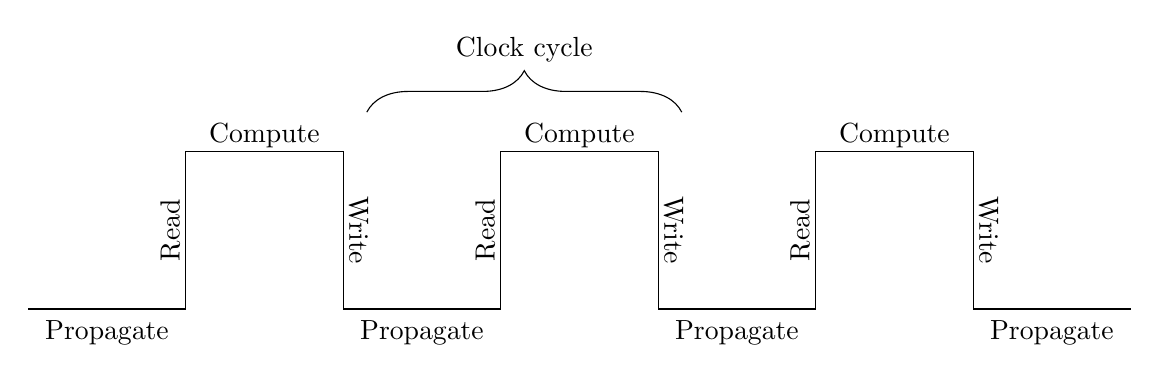
\begin{tikzpicture}
  \foreach \i in {0,4,8}
  \draw (\i,0) -- (\i+2,0) -- node [xshift=-0.2cm,rotate=90] {Read} (\i+2,2) -- node
  [yshift=0.2cm] {Compute}(\i+4,2) -- node [xshift=0.2cm,rotate=270] {Write} (\i+4,0);
  
  \draw (12,0) -- (14,0);
  \node [] at (13,-0.3) () {Propagate};

  \draw [decorate,decoration={brace,amplitude=15pt}] (4.3,2.5) -- (8.3,2.5) node
  [midway,yshift=0.8cm]{Clock cycle};

  \foreach \i in {0,4,8} {
  \node [] at (\i+1,-0.3) () {Propagate};
  % \node [blue] at (\i+3,-0.5) () {Run};
}

\end{tikzpicture}}
\caption{Illustration of the SME clock cycle concept.}
\label{fig:smeclock}
\end{figure}


% Even though you may already have realized the properties and components of the
% SME model, we give a more formal introduction here.

% A clock signal has four different states. Its either low, raising, high or
% falling. Conceptually, SME processes reads their input on the raising edge, then
% does computation, before writing the result of the communication.

% As referenced previously, the CSP concept of external choice was not found to be
% a good fit for hardware design, The key insight of the SME model is the concept
% of a \textit{hidden clock}


\subsubsection{An example}
\begin{figure}
  \centering
  \resizebox{.5\linewidth}{!}{
    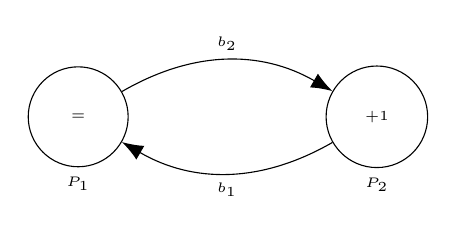
\begin{tikzpicture}[font=\tiny,
      proc style/.style={circle,draw=black,align=center,text
        width=1cm,minimum size=1cm,align=center}
      ]
      \node[proc style] (id) {$=$};
      \node[below=0cm of id] (p1) {$P_1$};
      \node[proc style,right=2.5cm of id] (add) {$+1$};
      \node[below=0cm of add] (p2) {$P_2$};
      \draw[-{Latex[scale=1.6]}] (id) edge [bend left=30] node [above] {$b_2$} (add);
      \draw[-{Latex[scale=1.6]}] (add) edge [bend left=30] node [below] {$b_1$}
      (id);
    \end{tikzpicture}
    }
    \caption{A simple SME network consisting of two processes. One simply
      forwards the received value while the other increments it by one.}
  \label{fig:smeint}
\end{figure}

Even though the concepts of the SME model are uncomplicated, gaining an
intuition of value propagation governed by globally synchronous semantics is
harder. In an attempt to convey this intuition, we show an example of a simple
network, seen in \Cref{fig:smeint}. We return to a slight variation of this
example later, but for now, the network consist of two processes $P_1$ and $P_2$
and two buses connecting them, $b_1$ and $b_2$. In this network, a value is
passed around in a circular fashion. The process $P_1$ simply forwards the value
it receives while the $P_2$ process increments it by 1.\begin{figure}
  \centering
  \begin{tabular}{c|cccccccccc}
    %\toprule
    \diagbox[height=1.6em]{op}{c} & 1 & 2 & 3 & 4 & 5 & 6 & 7 & 8 & 9  \\\hline
    $P_1 \leftarrow b_1$          & 0 & 1 & 1 & 2 & 2 & 3 & 3 & 4 & 4  \\
    $P_1 \rightarrow b_2$         & 0 & 1 & 1 & 2 & 2 & 3 & 3 & 4 & 4  \\
    $P_2 \leftarrow b_2$          & 0 & 0 & 1 & 1 & 2 & 2 & 3 & 3 & 4  \\
    $P_2 \rightarrow b_1$         & 1 & 1 & 2 & 2 & 3 & 3 & 4 & 4 & 5  \\
    %\bottomrule
  \end{tabular}
  \caption{A table showing values read and written for every clock cycle of SME
    networks. Note that when we refer to a {\itshape trace} later, it is
    different from the table shown here. An SME trace file normally only
    contains the values of the reading ends of bus channels following every
    cycle.}
\label{tab:trace}
\end{figure}
In \Cref{tab:trace} we see the actual values read and written by every process
for every cycle. Note that before every cycle shown in the table, an implicit
bus propagation is run, driving forward the bus values. The arrows denote the
operation performed. A process can either {\itshape write into} or {\itshape
  read from} a bus. So, the operation $P_1 \rightarrow b_1$ means that $P_1$
writes to $b_1$. The reading-ends of all buses initially start out as 0. Thus,
in the first cycle, this value is read by both processes. In the second cycle,
we see the effect of the delayed value propagation: $P_2$ reads 0 again, even
though it wrote 1 in the previous cycle. Due to the single-cycle delay in value
propagation through a bus, the 0 read now in cycle $c$ was written by $P_1$ in
cycle $c-1$. This pattern continues and we show the first 9 cycles here. In
cycle 9, the value written by $P_2$ is 5.
% If value propagation
% was immediate


\begin{figure}
  \centering
  \resizebox{.9\linewidth}{!}{
    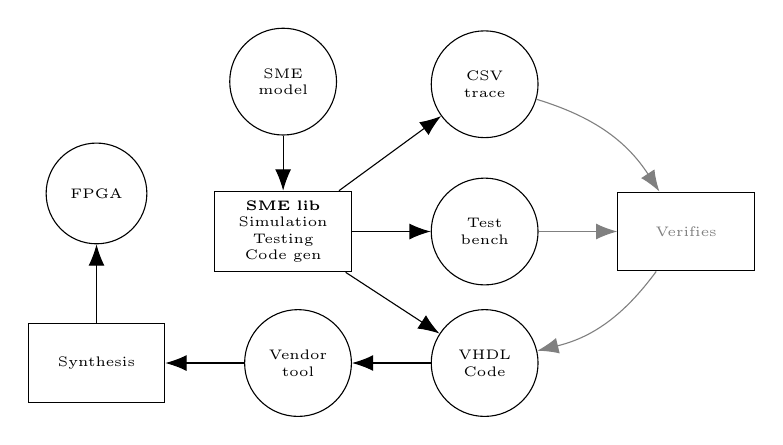
\begin{tikzpicture}[font=\tiny,
      rep style/.style={rectangle,draw=black,text width=1.5cm,minimum
        size=1cm,align=center},
      proc style/.style={circle,draw=black,align=center,text
        width=1cm,minimum size=1cm,align=center}
      ]
      \node[proc style] (impl) {SME model};
      \node[rep style,below=0.7cm of impl] (sim) {{\bfseries SME
        lib}\\Simulation\\Testing\\Code gen};
      \node[proc style,right=1cm of sim] (tb) {Test bench};
      \node[proc style,above=0.5cm of tb] (trace) {CSV trace};
      \node[proc style,below=0.3cm of tb] (code) {VHDL Code};
      \node[gray,draw=gray,rep style,right=1cm of tb] (verifies) {Verifies};
      \node[proc style,left=1cm of code] (vendor) {Vendor tool};
      \node[rep style,left=1cm of vendor] (synth) {Synthesis};
      \node[proc style,above=1cm of synth] (fpga) {FPGA};


      \draw[-{Latex[scale=1.6]}] (impl) edge [] (sim);
      \draw[-{Latex[scale=1.6]}] (sim) edge [] (trace);
      \draw[-{Latex[scale=1.6]}] (sim) edge [] (tb);
      \draw[-{Latex[scale=1.6]}] (sim) edge [] (code);

     \draw[-{Latex[scale=1.6]}] (trace) edge [gray, bend left=20] (verifies);
     \draw[-{Latex[scale=1.6]}] (tb) edge [gray] (verifies);
     \draw[-{Latex[scale=1.6]}] (verifies) edge [gray, bend left=20] (code);

     \draw[-{Latex[scale=1.6]}] (code) edge [] (vendor);
     \draw[-{Latex[scale=1.6]}] (vendor) edge [] (synth);
     \draw[-{Latex[scale=1.6]}] (synth) edge [] (fpga);

    \end{tikzpicture}}
    \caption{A simplified overview of the steps taken from SME model to hardware
    implementation.}
  \label{fig:smeflow}
\end{figure}

\subsection{Using SME}
% The key advantage of SME is that a low-level hardware description may be
% generated form an SME network written in a high-level language.

The purpose of modeling a design in SME is to eventually convert it to an actual
hardware description. Regardless of which SME implementation is used (including
the one described in this thesis), the process goes through the same general
steps shown in \Cref{fig:smeflow}. The first step is to write the SME model and
related tests in a language with the required SME support. Then, this model is
read by the SME library which simulates the design and runs the related tests in
order to verify correctness. Three results are generated from the simulation: A
rendering of the SME design in a HDL (only VHDL has been used so far), a
test-bench written in the HDL used for verifying the generated code and finally,
a CSV-file containing a value trace. The CSV-file is read by the test-bench
which uses it as a source of input values to provide to the hardware model and
for checking that its output values are as expected. The generated HDL code is
then passed to a vendor tool for synthesis and eventual implementation on
hardware.

The present work only affects the stages up until passing the generated HDL to a
vendor tool.


% Regardless of
% which specific SME implementation is used, the workflow from SME model to
% hardware implementation generally follows the same steps seen in
% \Cref{fig:smeflow}. First, an SME implementation written in a general-purpose
% language is simulated, using a self-hosted simulator. The result of this
% simulation is a trace file containing the values of the reading-ends of buses
% for every cycle. The code is then translated to VHDL code and a test-bench for
% testing the generated code. The test-bench will, using the values of the trace
% file, cycle-for-cycle, test the generated code.

% The purpose of all ``model'' SME implementation is to eventually generate a
% hardware description.  Furthermore, verification of the generated VHDL code is simplified
% since also a test-bench is generated. An overview of the process is shown in
% \Cref{fig:smeflow}. We show this, to give an understanding of what are the
% phases of a normal SME workflow. 



\subsection{Implementations}
A number of different library implementations of the SME model exists.

\subsubsection{\nth{1} PySME}
The initial implementation of SME was extremely simple: A mere 69 \gls{sloc} of
Python was all that was needed to create a library allowing Python programs to
be written following the SME model. This implementation was, of course, quite
rudimentary, however, it underlines a key advantage of the SME model. A person
can both understand the model and write an implementation from scratch in less
than a day.

\begin{widefigure}
  \centering
  \begin{minipage}{0.49\textwidth}
    \centering
    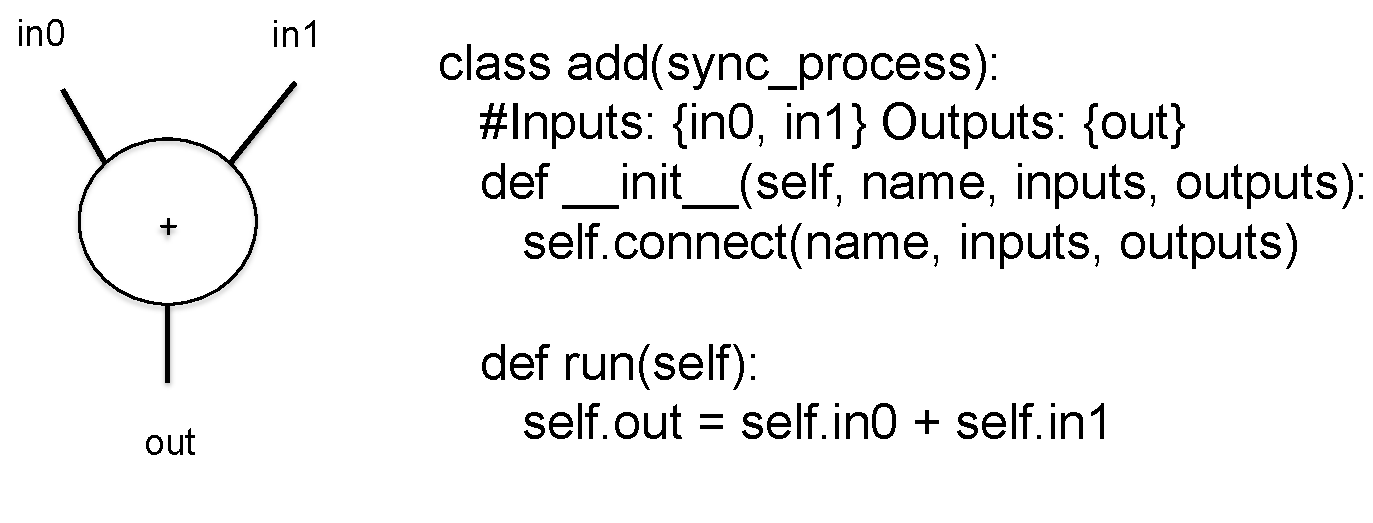
\includegraphics[width=.9\textwidth]{figures/add}
  \end{minipage}
  \begin{minipage}{0.49\textwidth}
    \centering
    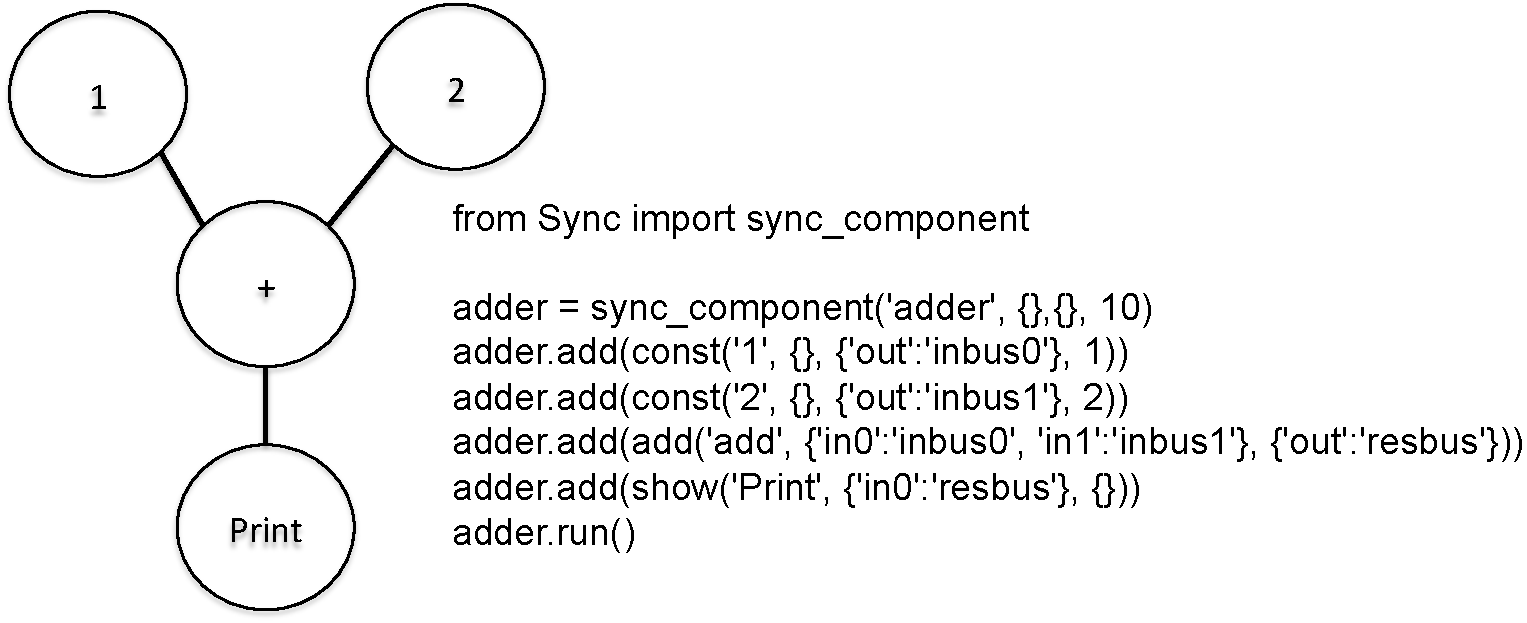
\includegraphics[width=\textwidth]{figures/addnet}
  \end{minipage}
  \caption{An implementation of an adder in the original SME framework. Figure
    from~\cite{vinter2014synchronous}.}
  \label{fig:adder}
\end{widefigure}

An example of a network for adding together two values written using this SME
implementation is seen in \Cref{fig:adder}. As can be seen, this initial SME
version created connections between processes using {\itshape named
  channels}. So connecting a channel between two processes was done just by
referencing the same name as an input port and output port in the instances of
two different processes.


\subsubsection{\nth{2} PySME}
After promising experiences with the first version of SME a revision to the
model and its implementation was published~\cite{vinter2015bus}. This version
contained a number of changes, the most important being the abandonment of using
the aforementioned named channels for connecting processes. Instead, buses were
now considered first-class independent components of an SME
network. Furthermore, a bus was extended from being just a single channel to a
bundle of channels. Also included was a new top-level construct, named
\texttt{Network} used purely for defining buses and their connections to
processes. The adder shown in \Cref{fig:adder} using this version of SME is seen
in \Cref{fig:adder2}.

Modeling buses as active components of the network opened up a number of
possibilities, in particular generating the CSV trace-files mentioned above. A
disadvantage of this approach was that defining the connections of a complex
network quickly became unwieldy, as may already be visible from the very short
example in \Cref{fig:adder2}.

At this point, SME was only used for simulation and prototyping of hardware
designs. The completed prototypes were then manually translated to \gls{vhdl}
and verified using the trace-file generated by simulating the original SME
implementation. This was a tedious process, but it showed the viability of
translating SME models to a hardware description.


% After an initial experience with the first version of PySME the SME model was
% updated~ to include some changes that was deemed useful. The
% most noticeable change, was the abandonment of connecting processes through
% CSP-like singular channels in favor of Buses as described above. As buses were
% implemented as active participants in the network , it was now possible to use the buses
% to save a trace of the values flowing through the network. This allowed
% continuing verification when SME models was manually translated to VHDL,
% simplifying ensuring correctness of the generated code. Furthermore, this
% version of SME extended buses to be a collection of channels rather than just 

\begin{widefigure}
  \begin{multicols}{2}
    \small
\begin{lstlisting}[language=python]
from bSME import *

class Const(Function):
  # [..]

class Add(Function):
  def setup(self, args):
    self.cbus1, self.cbus2, self.out = args
    self.out["val"] = 0
  def run(self):
    self.out["val"] = self.cbus1["val"] +
                      self.cbus2["val"]

class Printer(Function):
  # [..]

class Adder(Network):
  def wire(self, args):
    self.constbus1 = Bus("Const1", "val")
    self.constbus2 = Bus("Const2", "val")
    self.resbus = Bus("Result", "val")
    self.c1 = Const("c1", [self.constbus1, 30])
    self.c2 = Const("c2", [self.constbus2, 5])
    self.add = Add("add", [self.constbus1,
                 self.constbus2,
                 self.resbus])
    self.printer = Printer("print",
                           [self.resbus])
Adder("Adder").clock(10)
\end{lstlisting}
  \end{multicols}
\caption{The adder shown in \Cref{fig:adder} implemented using the updated
  version of the SME framework.}
\label{fig:adder2}
\end{widefigure}

\subsubsection{C\# SME}
A C\# implementation of the new version of SME was also
created~\cite{skovhede2016building}. The primary change from the Python SME
implementations was the omission of a {\ttfamily Network}-like
construct. Instead, connections between a pair of processes was established if
they referenced the same bus. So instead of process instances being
parameterized with their connections, processes established connections
themselves by referencing buses. This proved to be a more comprehensible way of
building networks as the information about connections was spread out throughout
the program instead of being confined in a single class.  However, a shortcoming
of this approach was the one-to-one correspondence between process and bus
declarations and instances. This limitation was alleviated in later versions of
C\# SME library by the introduction of {\itshape scopes} which allowed several
instances of the same process to exist as long as they were defined in different
scopes.

This version of SME also facilitated automatic translation to \gls{vhdl}.

\subsubsection{\nth{3} PySME}
Based on the success of translating SME models written in C\# to VHDL, a project
was started to bring the same capability to the Python version of
SME~\cite{asheim2016vhdl}. The challenges of deriving static code from a dynamic
language were briefly mentioned in the introduction. Due to this, the previous
PySME implementation altered to require the programmer to state her intentions
more clearly. For example, in the \nth{2} PySME, declaring a bus or
instantiating a process could be done simply by assigning a variable in the
{\ttfamily wire} function of a network class. This made analyzing the code
difficult, since the programmers intention was not clearly stated. Thus, an
{\ttfamily add} method was added to the \texttt{Network} class. This is the
version of PySME used in the thesis.

\subsubsection{Conclusions}
The design of SMEIL draws heavily from the lessons learned by the different
approaches used by these SME implementations. 
% We have drawn two conclusions from the differing approaches used by C\# SME and
% the \nth{2} PySME which has influenced the design of SMEIL.
First of all, we concluded that requiring all buses and connections to be
declared in one place quickly become difficult to understand. The other is, that
it would be advantageous to associate process instances with bus instances to
avoid the same pitfall as the original C\# implementation. This also helpful
when using SMEIL as an \gls{il} since buses and their connections translated
straightforwardly regardless of the originating implementation.


%%% Local Variables:
%%% mode: latex
%%% TeX-master: "../master"
%%% End:

\chapter{Hardware Description Languages}
\todo{Write this}. Give a brief overview of a hardware design workflow and give
an overview of especially VHDL as this is discussed here repeatedly.

%%% Local Variables:
%%% mode: latex
%%% TeX-master: "../master"
%%% End:

%\chapter{Analysis}

\section{Definition Structure}
Early descriptions of \gls{sme} defined networks in a rather rigidly, by
requiring all buses, process instantiations and links between them to be placed
within a network definition. Building \gls{sme} networks in this manner proved
limiting and confusing as it was easy to loose track of how buses within a
network was connected. The C\# implementation of \gls{sme} loosened this
restriction by defining buses directly within processes. Connections between
processes was then created simply by referring to a bus within another
process. This proved, in practice, to be much more programmer friendly as it
made the connections between processes easier to reason about. The limiting
factor of this design was the bijective relationship between process
declarations and their instances. Overcoming this limitation in practice
required the inelegant use of plain-text templates for creating multiple
duplicate process and network definitions. To remove this limitation, support
for ``Scopes'' was added to C\# \gls{sme}. Scopes a

Each network definition creates an enclosed scope around the processes it
instantiates. Therefore, processes from other networks may only connect to buses
which are exposed through another network definition. 

\section{Network Instantiation}
Instantiation of process networks defined in \gls{smeil} is a topic which
deserved particular attention. In \gls{sme} libraries for general-purpose
languages, the networking structures are explicitly defined and network
instantiations happen naturally when the code is execution. The actual
instantiation process here is, as we might say, handled by the programming
language that the networks are instantiated within. For \gls{smeil} we aren't as
lucky and a method needed to be developed. Valid \gls{sme} networks are
representable as a connected directed acyclic graph. Acyclicity is a required
property as we would otherwise end up with infinite instantiation loops. The
buses of \gls{sme} networks may, however, form loops. Once the graph has been
created and we have shown the graph to be acyclic, we topologically sort the
nodes and start instantiating the network from the first node in the sorted
nodelist.  TODO: Show examples and write some more about this. The method of
instantiation for \gls{sme} networks is summarized as follows:
% \begin{itemize}
% \item Construct a graph from \gls{sme} network definitions
% \item Show that graph is acyclic
% \item Perform a topological sort of nodes in the graph. Instantiate the network
%   from the first entry of this graph. Alternatively, simply start from the node
%   with in-degree of 0. (TODO: Is this valid?)
% \end{itemize}

TODO: Clarify relationship between instantiation graph and connection graph.

%%% Local Variables:
%%% mode: latex
%%% TeX-master: "../master"
%%% TeX-command-extra-options: "-enable-write18"
%%% End:

\chapter{The SME Implementation Language}

The language introduced in this thesis, the \gls{smeil}, is a small, strongly and
statically typed, C-like language featuring SME primitives as first-class
constructs.
% The
% star of the thesis, SMEIL, can be seen as a ``c-light'' language featuring SME
% primitives as first-class constructs
In this section, we give an (informal) introduction to its syntax and semantics.

%\todo{Rewrite. Replace with mini SMEIL intro}
% The \gls{smeil} project started out with the intention of purely creating an
% intermediate language, However, as previously stated, it evolved into an
% independent \gls{dsl} for describing \gls{sme} networks. Therefore, we did not
% initially spend a lot of time investigating alternative \gls{hdl}.

%\section{Design Rationale}
\section{Guiding Principles}
As mentioned in the introduction, the initial design decisions of \gls{smeil}
were primarily driven by the goal of providing a straightforward mapping of
constructs found in languages such as Python and C\#. These two languages, in
particular, were the initial focus since they already had \gls{sme}
implementations with code generation backends for \gls{vhdl}. Thus, the SME
implementations were proven capable of more than just simulating simple SME
networks. Furthermore, taking two imperative languages with different typing
disciplines into consideration meant that \gls{smeil} was less likely to adopt
idiosyncrasies of either statically or dynamically typed languages. The body of
SME code already existing for Python and C\#, also meant that we could do more
than just hypothesizing about the consequences of our SMEIL design
choices. Furthermore, it allowed us to identify common use-patterns in order to
help determining the requirements of an SME language.

% This use-pattern based
% design process \todo{finish or remove} In the design of the language, the
% primary emphasis is on making life easy for


Thus, the four guiding principles driving the initial design of the language
were phrased as:
\begin{description}
\item[Language independence.] Since SME networks can be written in several
  different languages, SMEIL should have no elements which are specific to a
  certain source language.
\item[Structural richness.] A goal of the SME model is that the generated code
  should be readable and have a relationship with the original source
  code. Therefore, SMEIL should have rich constructs for specifying the
  structure of SME networks.
\item[Readability.] Ensuring that the language has a readable and accessible
  representation aids debugging and makes it possible to understand For this
  reason, SMEIL has a human-readable concrete syntax.
\item[Composability.] The language should provide unrestricted composability to
  ensure that networks can be subdivided for optimal flexibility.
\item[Principle of least astonishment.] Constructs in SME resembling constructs
  found in popular general-purpose programming languages will probably do the
  same thing. As a continuation of the goal to ensure a straight-forward mapping
  of, for example. C\#, the semantics of things which are not directly SME
  related are what you would expect. This principle applies everywhere in the
  language except for reading to and writing from bus channels. As these are
  features unique to SME.
  % it is hard to give them a syntax which is convenient,
  % while, at the same time, unrecognizable from features in other languages.
  % TODO: Something about the strictest possible subset by default?
\end{description}



As we also alluded to in the introduction, the third principle on the list
above, {\itshape Readability}, required SMEIL to have a human readable concrete
syntax. However, very early on, we explored simply having an intermediate
representation, using JSON as its encoding, for exchanging \gls{smeil} programs
between frontends and backends. However, aside from the goal of readability, the
design of a representation having no concrete syntax also proved tedious since
it was impossible to reason about ``code'' which did not have an intuitive
representation.

The C-like syntax of SMEIL was chosen since it is simple to parse and contains
no significant whitespace. Furthermore, curly-braces are used to clearly
distinguish blocks and semicolons clearly mark the end of statements.
 
% In compiler literature, (e.g. Mogensen .. )The term \textit{Intermediate
%   Language} is commonly associated with languages that sit at a lower level of
% abstraction than the source languages that they are targeted by. They are
% commonly introduce to make program transformation and optimization easier by
% removing syntactic sugar and other niceties that make a programming language
% easy to work with for humans. The goal of SMEIL is somewhat different...  Since
% we exclusively target other high-level languages which are intended as primary
% implementation languages for their respective domains, implementing classic
% language optimization techniques (e.g. constant expression folding,
% copy-propagation, etc...) is bring any benefit. In fact, since these
% optimizations are implemented by compilers for our target languages it may
% actually work against us since producing already-optimized source code may hide
% opportunities from the target compilers causing them to generate less efficient
% code. At the very least, due to the variety of destination languages that we
% support, we cannot make any general assumptions about which optimizations that
% would be beneficial. Optimizations specific to destination languages, however,
% may prove to be beneficial, but exploring this angle is outside the scope of
% this thesis.

% In designing SMEIL, we therefore opted for what we refer to as ``structural
% richness''


%\gls{SMEIL} 

\section{Language reference}
\label{sec:langref}
In this section, we describe the SMEIL language and its grammar from beginning
to end. Following this introduction, we look a small example to show how it all
comes together. The grammar of SMEIL (in BNF format) is presented as fragments
as we go along. Note that all the grammar fragments come together, so one
fragment may refer to a production declared in another fragment. We have done
our best to make sure that productions only refers to productions declared
before them, not ahead, however, this was not always possible.

% For network.

% There is no requirement for a \gls{sme} language to have a network construct

%\subsection{Language Constructs}

%\setlength{\grammarparsep}{1pt plus 1pt minus 1pt} % increase separation between rules
\setlength{\grammarindent}{10em} % increase separation between LHS/RHS

\subsection{Modules}
\begin{grammar}
  <module> ::= \{ <import-stm> \} <entity> \\ \{ <entity> \}

  <import-stm> ::= `import' <import-name> <qualified-specifier> `;'
  \alt `from' <import-name> \\ `import' <ident> \{ `,' <ident> \} <qualified-specifier>
  `;'

  <import-name> ::= <ident> \{ `.' <ident> \}

  <qualified-specifier> ::= \{ `as' <ident> \}

  <entity> ::= <network>
  \alt <process>
\end{grammar}


The fundamental unit in an SMEIL program is a {\ttfamily module}. Similarly to,
e.g., Python, a module corresponds to a file. Unlike Python, only files can be
modules and we don't provide a way to make a directory act as a
module\footnote{In Python, this is done by creating a {\ttfamily
    \_\_init\_\_.py} file in a directory}. Hierarchies of modules are built by
including one or more entities defined in a foreign module. Allowing SMEIL
programs to be separated in several files makes it simple to split
implementations up into reusable components. A module contains import-statements
and entities (described next). The syntax and semantics of import statements,
are equivalent to those of Python and will be familiar to an experienced Python
programmer. The handling of modules in SMEIL is described further in
\Cref{sec:overview}.

As an alternative to the current module system, we considered a model simply
based on source includes. The implementation of such a system would be similar
to that of the C pre-processor, possibly with implicit include guards preventing
a single file from being imported more than once. The primary problem with this
approach, despite being simpler to implement, is that include-based ``module''
systems feel archaic and require the names of all modules to be
unique. C-libraries gets around this by, as a convention, prefixing all function
names with the name of the library, however this is not a very elegant solution.

The module system of SMEIL contributes towards the goal of creating reusable
component libraries for SME. \todo{Did we mention that this was a goal?}


% The fundamental building blocks of SME models are networks and processes. A
% process is a concurrently run block of sequential code while networks describes
% the invocations of

\subsection{Entities}
\begin{grammar}
  <network> ::= `network' <ident> `(' [ <params> ] `)' \\`{' <network-decl> `}'

  <process> ::= [ `sync' | `async' ] `proc' <ident> \\ `(' [
             <params> ] `)' \{ declaration \} `{' \{ <statement> \} `}'

  <network-decl> ::= <instance>
  \alt <bus-decl>
  \alt <const-decl>
  \alt <gen-decl>

  <declaration> ::= <var-decl>
  \alt <const-decl>
  \alt <bus-decl>
  \alt <enum>
  \alt <function>
  \alt <instance>
  \alt <generate>
  
  <param> ::= \{ `[' \{ <expression> \} `]' \} <direction> <ident>

  <params> ::= <param> \{ , <param> \}

  <direction> ::= `in' (input signal)
  \alt `out' (output signal)
  \alt `const' (constant input value)  
\end{grammar}

SMEIL programs are composed of two basic building blocks: {\ttfamily
  process} and {\ttfamily network}. Together, we refer to them as {\itshape
  entities}. Network entities may only contain declarations which are static at
compile-time. Thus, the purpose of networks is purely to define relations
between entities.  Processes consist of a declarational part and a procedural
part (the body). The declarational part defines all the variables and buses used
in a process while the body is a collection of sequential statements which are
evaluated once per clock cycle.

To simplify program analysis, it is not possible to declare new variables inside
the body of a process. All variables used in the body must therefore be declared
in the declarational part of the process ahead of use. We considered if this
would unduly inconvenience users of SMEIL: For users of SMEIL as an intermediate
language, the inconvenience is very slight since it is easy to gather all
variables used in a code block and add declarations. Human users will be
slightly more inconvenienced, however, they were not part of the original design
considerations.

As can be seen from the grammar, networks may only contain static
declarations. The reason for this is that the structure of an SME network must
be static at compile time. Due to the static target of SMEIL, it is impossible
to, for example, instantiate new processes at runtime.

A related question to ask is, why make the distinction between networks and
processes in the first place? After all, all declarations which are allowed in
a network is also allowed in the declarational part of a process. \todo{Why is this?}

\todo{Explain the sync and async keywords}
\todo{Explain that entities may be parameterized}
\todo{Show examples of network and processes}

%At the top level, modules consist of network- and process declarations. 

All well-formed SMEIL networks must contain a {\tt network} declaration which is
used as the top-level entity containing the exposed interfaces of the
network. The top-level network is determined as follows: A graph is generated
from the SMEIL network containing one node per entity and edges between entities
that instantiate each other. The nodes of the graph are then topologically
sorted and the head of the sorted list is the top-level entity of the
network. We also ensure that the graph is acyclic as process instantiation
cycles would expand indefinitely. Note that even though the connections of a
network such as AddOne (Seen in \Cref{sec:smeilex}) is cyclic, its
instantiation graph is not since a single network instantiates the two
processes.


\subsection{Declarations}
This section describes the declarations that may occur in {\ttfamily network}s
and the declarational parts of {\ttfamily processe}s. Note that an {\itshape
  <expression>} occurring in declarations must be compile-time
static. Furthermore, due to limitations of the current compiler implementation,
they are in some cases limited to integers.

\subsubsection{Variables and constants}
\begin{grammar}
  <var-decl> ::= `var' <ident> `:' \\ <type-name> [ `=' <expression> ] [ <range> ] `;'

  <range> ::= `range' <expression> `to' <expression>

  <const-decl> ::= `const' <ident> `:' <type-name> [ `=' <expression> ] `;'
\end{grammar}

Variables and constants are what you would expect: Variables and
constants. Constants are used for declaring named constant values, for instance
\begin{lstlisting}[language=smeil]
const secs_per_hour: uint = 3600;
\end{lstlisting}
Constants should always be declared with an unbounded type (see
\Cref{sec:typesys}) as it allows for more accurate type unification. Due to
this, the compiler will emit a warning for constants declared with constrained
types, such as {\ttfamily u8}.

Variables allow for defining process-local mutable values. A semantic variation
compared to general-purpose languages is that variables in SMEIL is that the
state of a variable persists between process runs (clock cycles). In a way, they
are similar to function-local {\ttfamily static} variables in C whose value
persists between function calls.

In addition to a type, variables may also take a specified {\ttfamily range} of
values. For example, the following declarations
\begin{lstlisting}[language=smeil]
var seconds: uint range 0 to 59 = 0;
var seconds: u6 range 0 to 59 = 0;
var seconds: u6 = 0;
\end{lstlisting}
are all equivalent. The following declaration, on the other hand,
\begin{lstlisting}[language=smeil]
var seconds: u4 range 0 to 59 = 0;
\end{lstlisting}
is rejected by the type checker since representing the number $59$ requires more
than 4 bits.

The assignment ({\ttfamily = 0}) of all of these declarations sets the initial
value of the variable.

The {\ttfamily range} option was primarily added as a way to provide an
intuitive way of specifying the expected range of a variable. However, a further
use is described in \Cref{sec:typing}. Currently, the given range is only used to
calculate the number of bits required to hold the value. Only the range given by
the bit-size is enforced during simulation. This is to more closely mimic the
resulting hardware implementation.

\subsubsection{Enumerations}
\begin{grammar}
<enum> ::= `enum' <ident> `{' <enum-field> \{ `,' <enum-field>  \} `}' `;'

<enum-field> ::= <ident> [ `=' <integer> ]
\end{grammar}

Enumerations are a useful way of specifying closely associated named numerical
constants. They are used in a number of a designs made with the C\# SME library,
for example, in the MIPS processor implementation~\cite{johnsen2017thesis} where
the MIPS opcodes are defined in an {\ttfamily enum}. This improves code
readability by referencing symbolic constants instead of numeric
constants. Thus, to fulfill our goal of providing straightforward mappings from
constructs commonly used in other SME implementations, enumerations were added
to SMEIL.

Semantics are similar to other C-like languages. For example,
\begin{lstlisting}[language=smeil]
enum numbers {
  zero,
  three = 3,
  four,
  ten = 10
};
\end{lstlisting}
declares the enumeration {\ttfamily numbers} where the members are named in
correspondence with their numeric values.

\todo{Write about how enums are typed as integers and the limitations
  originating thereof, maybe}

\subsubsection{Bus declarations}

\begin{grammar}
<bus-decl> ::= [ `exposed' ] [ `unique' ] `bus' <ident> \\ `\{' <bus-signal-decls> `\}'  `;'

<bus-signal-decls> ::= <bus-signal-decl> \{ <bus-signal-decl> \}

<bus-signal-decl> ::= <ident> `:' <type> [ `=' <expression> ] [ <range> ] `;'
\end{grammar}

The perhaps most interesting of the declarations described here are buses. As
previously mentioned, buses in SME are used for communication between
processes. They provide a collection of one or more channels, of varying types,
which are assigned to processes as a single entity (i.e., all channels of a bus
are connected at the same time). The cardinality of buses is unrestricted,
meaning that they may form many-to-many relationships between processes. Thus,
SME buses mirrors hardware buses, realized as physical wires, where many
components may be connected to the same wire. As a consequence of this, a bus
may only have a single {\itshape driver} (an entity sending a signal on the bus)
per clock cycle, since otherwise, the signal read from the bus is {\itshape
  unresolved} (i.e., its value is undecidable).

A bus in SMEIL is declared using a {\ttfamily bus} block. For example
\begin{lstlisting}[language=smeil]
exposed bus pixel {
  r: u8;
  g: u8;
  b: u8;
};
\end{lstlisting}
declares a bus named {\ttfamily pixel} used for transmitting the pixels of an
image separated into their red, green and blue color channels. It contains three
individual channels named {\ttfamily r}, {\ttfamily g} and {\ttfamily b} each of
which is typed as 8-bit unsigned integers. The {\ttfamily exposed} modifier
signifies that the bus is used for external interactions, either through
co-simulation (\Cref{sec:cosim}) or through the generated VHDL test bench
(\Cref{sec:codegen}).

Exposed buses must be defined within, or in entities directly instantiated from,
the top level entity. Otherwise incorrect code will be generated. It is a future
goal to check this statically such that appropriate error messages are emitted.

Similarly to variables, mentioned above, bus channels allow the specification of
a {\ttfamily range}.

Another modifier for buses is the {\ttfamily unique} keyword. Unfortunately, it
is not currently implemented. The intent behind this was to allow buses with
multiple writers. \todo{finish}

% \begin{figure}
%   \centerfloat
% \begin{subfigure}[width=0.4\paperwidth]
% \begin{lstlisting}[language=smeil]
% proc A ()
% bus b {
%   chan: int;
% };

% \end{lstlisting}
% \end{figure}

\subsubsection{Entity instances}
\label{sec:instance}
\begin{grammar}
  <instance> ::= `instance' <instance-name> `of' <ident> \\`(' [ <param-map> { `,' <param-map> } ]`)' `;'

  <instance-name> ::= <ident> `[' <expression> `]' (indexed instance)
  \alt <ident> (named instance)
  \alt `_' (anonymous instance)

  <param-map> ::= [ <ident> `:' ] <expression>

\end{grammar}

A powerful feature of SME is its ability to define compositions of reusable
networks. In SMEIL, networks are constructed by instantiating entities and
connecting them using buses. Possible ways of composing a network is subject to
only a few restrictions.

It is often convenient to have several instances of the same process that are
parameterized with different connections or different constant
values. Therefore, both processes and networks have parameters which are set
upon instantiation. Three types of parameters are supported: input- and output
buses and constants. The {\tt instance} statement is used to instantiate an
entity with a specified set of parameters. An instance may optionally be given a
name which can be used for referencing buses declared within the instantiated
entity. \Cref{fig:comms} shows three different ways that a network may be
constructed through bus references. If an instance is unnamed (anonymous),
connections between the instances can be made by referring to buses through
their public names\todo{Add reference to figure}.

Several anonymous instances of an entity may exist within the same network. To
avoid ambiguous networks, a scope may only contain a single anonymous instance
of a particular entity.  \Cref{fig:anonproc} shows two network utilizing
anonymous entity instances. They both attempt to create the same number of
instances of each process, however, one makes two anonymous instantiations from
the same process and is thus invalid.

Also note that {\itshape <instance-name>} allows the name of an instance to be
followed by an optional array index (e.g., {\ttfamily instance a[i] of ..}),
creating an {\itshape indexed instance}. This is intended to be used together
with {\ttfamily generate}-declarations (described below) in order to create an
array of instances. Like {\ttfamily generate}-statements, this feature is
unfortunately not currently implemented.

\begin{widefigure}
  \begin{subfigure}[t]{0.33\textwidth}
    \begin{lstlisting}[language=smeil]
proc A ()
bus b_a { chan: int; };
{ B.b_b.chan =
  b_a.chan; }

proc B ()
bus b_b { chan: int; };
{ A.b_b.chan =
   b_a.chan; }

network N ()
{ instance _ of A();
  instance _ of B();
}
\end{lstlisting}
  \caption{A network created by processes directly using buses through their
    hierarchical declarations.}
  \end{subfigure}
  \begin{subfigure}[t]{0.33\textwidth}
    \begin{lstlisting}[language=smeil]
proc A (in i)
bus b_a { chan: int; };
{b_a.chan = i.chan; }

proc B (in i)
bus b_b { chan: int; }
{b_b.chan = i.chan; }

network N () {
 instance a of
   A(b.b_a);
 instance b of
   B(a.b_b);
}
\end{lstlisting}
    \caption{A network created using processes taking their input bus as a
      parameter. The connection between the two processes is made by the network
      N.}
  \end{subfigure}
  \begin{subfigure}[t]{0.32\textwidth}
    \begin{lstlisting}[language=smeil]
proc A (in i, out o)
{ o.chan = i.chan; }

network N ()
{
  bus b_a { chan: int; }
  bus b_b { chan: int; }

 instance a of
   A(b_a, b_b);
 instance b of
  A(b_a, b_b);
}
\end{lstlisting}
    \caption{This network only contains a single network taking both its input
      and output buses as parameters. The same network as in (a) and (b) is then
      built by passing bus references to two instances of {\tt A}.}
    
  \end{subfigure}

  \caption{The three different networks shown here are equivalent and
    demonstrates different ways of connecting processes in SMEIL.}
  \label{fig:comms}
\end{widefigure}

\begin{figure}
  \centering
  \begin{subfigure}[t]{0.40\textwidth}
\begin{lstlisting}[language=smeil]
proc B () {}
proc C ()
  instance _ of B();
{}
network N {
  instance _ of B();
  instance _ of C();
}
\end{lstlisting}
    \caption{Since the two anonymous instances of process {\tt B} are
      instantiated from different entities, this network is valid.}
    \label{fig:ambigvalid}
    \hspace{4mm}
\end{subfigure}
\begin{subfigure}[t]{0.40\textwidth}
\begin{lstlisting}[language=smeil]
proc B () {}
proc C ()
{}
network N {
  instance _ of B();
  instance _ of B();
  instance _ of C();
}
\end{lstlisting}
    \caption{The duplicate anonymous instances of {\tt B} in {\tt N} makes this
      network invalid.}
  \end{subfigure}

  \caption{Two networks showing a valid and invalid use (respectively) of
  anonymous entity instances.}
\label{fig:anonproc}
\end{figure}

When an entity is instantiated, a copy is created of all the resources declared
within it. In particular, instantiating a process containing a bus will also
create a new instance of that bus.
% If this is not desired for a bus, it may
% be declared with the \texttt{uniqe} modifier which commands that only a single
% instance of the bus is crated. This makes it possible to have a many-to-many bus
% having several instances as both readers and writers.


\subsubsection{Generators}
\begin{grammar}
  <gen-decl> ::= `generate' <ident> `=' <expression> `to' <expression> \\ `{' \{ <network-decl> \} `}'
\end{grammar}
The {\ttfamily generate} declaration adds limited the metaprogramming
capabilities to SMEIL. Unfortunately, it is not yet supported by the current
implementation. It is frequently desired to create networks with a parameterized
structure. For example, ... \todo{Add an example}

The semantics of {\ttfamily generate} statements are simple:
\begin{smeilcode}
generate i = 0 to 2 {
  instance a_inst[i] of a(val: i);
}
\end{smeilcode}
is equivalent to
\begin{smeilcode}
instance a_inst_1 of a(val: 1);
instance a_inst_2 of a(val: 2);
instance a_inst_2 of a(val: 3);
\end{smeilcode}
  
Critics could claim that the naming of this definition, which is inspired by
VHDL, adds unnecessary bloat to the language. Instead, a {\ttfamily for}-loop
could be used.  \todo{finish}

\subsubsection{Functions}
\begin{grammar}
  <function> ::= `func' <ident> `(' \{ <function-param> \} `)' `:' <type-name>
  \{ <declaration> \} `{' { <statement> } `}' `;'

  <function-param> ::= <ident> `:' <type-name>
\end{grammar}
\todo{Not implemented, but describe}

%%%%%%%%%%%%%%%%%%%%%%%%%%%%%%%%%%%%%%%%%%%
% REVIEW THIS
% Processes are instantiated using the \textsc{instance} keyword (syntax given
% below) allowing its parameters to be set. All the declared elements of a bus
% such as variables or buses are cloned for each declared instance. If a process
% is not explicitly instantiated, it can be referred to through its
% \textit{default instance}. Globally in the program, the default instance is
% referred the name of the process, while explicitly defined instances are
% referred to by the name of the instance. Let's consider a simple network
% containing a process accumulating a value, continuously accumulating the sum of
% three different numbers from three different sources: a value read from an input
% bus, a value defined as a constant parameter to a process and a value defined as
% a constant within the process itself. For each cycle, the accumulated value is
% written to an exposed result bus where it can be read out.

% In the first variation of this example, we declare two processes outputting
% constant values, using explicit instances
% %\inputminted[fontsize=\small]{c}{samples/addn.sme}

% Now we look at the second variation. This time, we only define a single process
% for generating a constant value and thus, we don't need to declare explicit
% instances for the value generating process.

% %\inputminted[fontsize=\small]{c}{samples/addn2.sme}

% We could further extend this by removing the \texttt{val} parameter of the
% \texttt{num} process, removing the need for any instances at all. The network
% declaration, however, is still required but may, in this case, be left empty.


% The scope of a bus declared within a process is inferred based on its use, such
% that buses only referenced from within the process itself are considered private
% buses. Since we can decide this unambiguously, only one visibility modifier for
% buses exists, the \textsc{exposed} modifier, which indicates that a bus is used
% as an external input for the network.
%%%%%%%%%%%%%%%%%%%%%%%%%%%%%%%%%%%%%%%%%%%%%%%%%%%%%%%%%

% \paragraph{Dynamically configured networks} The last thing we need to cover is
% how to generate dynamically configurable networks.. TODO: Write about how to
% parameterize number of buses.

% \paragraph{Semantics of interpretation} Statements in an SMEIL program are
% either declarative or imperative in nature. Generally, anything within a network
% block are considered declarative while anything in the body of processes are
% declarative in nature. Let us look at a third variation of the example above,
% this time allowing for parameterized network configurations.

% %\inputminted[fontsize=\small]{c}{samples/addn3.sme}

% By using array notation in the parameters of the \texttt{addN} process, we can
% specify that an array of signals are accepted as input. Looking at the network
% declaration, \texttt{addN_net}, we see how we can use the array index with
% instance names to create a compile-time dynamic number of instances.

% \paragraph{Functions.} Functions in SMEIL are...

% \paragraph{Templates.} The \texttt{generate} statement, with its nomenclature
% taken from VHDL, allows statement \textit{generation} (or templating) within
% \texttt{network} definitions. These are the primary means of which parameterized
% dynamically created network layouts are written.

\subsection{Statements}
\begin{grammar}
  <statement> ::= <name> `=' <expression> `;' (assignment)
  \alt `if' `(' <condition> `)' `{' \{ <statement> \} `}' \\ \{ <elif-block>
    \} [ <else-block> ]
  \alt `for' <ident> `=' <expression> `to' <expression> \\ `{' \{ <statement> \} `}'
  \alt `while' <condition> `{' \{ <statement> \} `}'
  \alt `switch' <expression> \\ `{' <switch-case> \{ <switch-case> \}
  [ `default' `{' <statement> \{ <statement> \} `}' ] `}'
  \alt `trace' `(' <format-string> \{ `,' <expr> \} )`;'
  \alt `assert' `(' <condition> [ `,' <string> ] )`;'
  \alt `barrier' `;'
  \alt `break' `;'
  \alt `return' [ <expr> ] `;'

  <switch-case> ::= `case' <expression> \{ <statement> \}

  <elif-block> ::= `elif `(' <condition> `)' `{' \{ <statement> \} `}'

  <else-block> ::= `else' `{' \{ <statement> \} `}'

  <format-string> ::= `"' { <format-string-part> } `"' `;'
  
  <format-string-part> ::= `{}' (placeholder string)
  \alt <string-char> (normal string char)
\end{grammar}

The semantics of statements in SMEIL corresponds to their counterparts in C-like
languages. Thus, we will not devote a lot of attention to describing them
here. A few things to note:

\paragraph{Assignments.} In assignments, we make no distinction about what is
being assigned. The same syntax is used whether buses or variables are being
assigned. A common trait of HDLs is that they make a syntactic distinction
between the two. VHDL, for example, uses \texttt{:=} and \texttt{<=} for
variables and signals respectively. In the design of SMEIL we concluded that
there was no need for making this distinction: The compiler is always able to
distinguish which kind of object is being assigned to based on the type that it
was declared as.

\paragraph{Loops.} \texttt{for}-loops have, compared to C, a slightly more
restricted syntax. For example, the following,
\begin{lstlisting}[language=smeil]
for i = 1 to 10 {
  trace("{}", i);
}
\end{lstlisting}
iterates through the range 1-10 (inclusive).\todo{Why is this?}

\paragraph{Tracing and Asserting.}The {\tt trace} and {\tt assert} statements of
SMEIL respectively reports on the state of the network and enforces runtime
constraints. A {\tt trace} statement takes a string optionally containing
replacement ``holes'' (similar to {\tt printf}) followed by a number of
arguments matching the number of holes. For example,
\begin{lstlisting}[language=smeil]
foo = 1; bar = 2;
trace("foo {} bar {}", foo, bar);
\end{lstlisting}
will print
\begin{verbatim}
foo 1 bar 2
\end{verbatim}
every time the process is executed.

Assertions are useful to specify invariants which must be maintained during
program execution. In SMEIL, {\tt assert} statements hold a condition and an
optional message. When an assert statement is evaluated, the condition is
checked, and program execution is halted if a condition is violated. If present,
the message is printed as part of the assertion error message.
\begin{lstlisting}[language=smeil]
assert(i > 10, "i must always be greater than 10");
\end{lstlisting}


\paragraph{Switch statements.} \texttt{switch} statements are similar to their
C-counterpart except for the omission of implicit fallthrough. There are two
reasons for this. The equivalent to a switch-statement in VHDL have no
fallthrough-capabilities built in. Furthermore, implicit fallthroughs are a
misfeature of C as they often lead to incorrect code containing unintentional
fallthroughs. There are plans to eventually add {\itshape explicit}
fallthroughs, although in order for this to be done, we need to find a way for
representing them in VHDL.

% \paragraph{General.} Finally, curly-braces are always required. Making
% curly-braces optional in some circumstances, are a misfeature of C-like
% languages.

\subsection{Expressions}
%\paragraph{BNF}
\begin{grammar}
  <expression> ::= <name>
  \alt <literal>
  \alt <expression> <bin-op> <expression>
  \alt <un-op> <expression>
  \alt <name> `(' \{ <expression> \}  `)' (function call)
  \alt `(' <expression> `)'

  <bin-op> ::= `+' (addition)
  \alt `-' (subtraction)
  \alt `*' (multiplication)
  \alt `/' (division)
  \alt `\%' (modulo)
  \alt `==' (equal)
  \alt `!=' (not equal)
  \alt `\verb!<<!' (shift left)
  \alt `\verb!>>!' (shift right)
  \alt `<' (less than)
  \alt `>' (greater than)
  \alt `>=' (greater than or equal)
  \alt `<=' (less than or equal)
  \alt `\&' (bitwise-and)
  \alt `|' (bitwise-or)
  \alt `^' (bitwise-xor)
  \alt `\&\&' (logical conjunction)
  \alt `||' (logical disjunction)

  <un-op> ::= `-' (negation)
  \alt `+' (identity)
  \alt `!' (logical negation)
  \alt `~' (bitwise-not)

\end{grammar}

The syntax of expressions the syntax and precedence rules (\Cref{tab:ops}) are
similar to those of C-like languages. Note that there is no notion of truthness
(see \Cref{sec:typesys}) and logical operators (e.g. \texttt{\&\&}) therefore only
accept boolean values. Relational operators (e.g. \texttt{<=}) returns a boolean
value as there result. \todo{do we need more?}


\begin{table}%[H]
  \centering
\begin{tabular}{cc}
  \toprule
  \textbf{Precedence} & \textbf{Operators}\\
  \midrule
  0 & \verb!+! \verb!-! \verb|!| \verb!~! (unary)\\
  1 & * / \% \\
  2 & + - \\
  3 & \verb!<<! \verb!>>! \\
  4 & < > <= >= \\
  5 & == != \\
  6 & \verb!&! \verb!^! \verb!|! \\
  7 & \verb!&&! \\
  8 & \verb!||! \\
  \bottomrule
\end{tabular}
\caption{Operator precedence of SMEIL}
\label{tab:ops}
\end{table}

\subsection{Lexical elements}
\todo{Shorten this or relate to other grammar}
%\paragraph{BNF}
\begin{grammar}

  <type> ::= `i' <integer> (signed integer)
  \alt `int' (arbitrary-width signed integer)
  \alt `u' <integer> (unsigned integer)
  \alt `uint' (arbitrary-width unsigned integer)
  \alt `f32' (single-precision floating point)
  \alt `f64' (double-precision floating point)
  \alt `bool' (boolean value)
  \alt `[' [ <expression> ] `]' <type> (array of type)


  <literal> ::= <integer>
  \alt <floating>
  \alt `"'\{ <char> \}`"' (string literal)
  \alt `[' <integer> \{ `,' <integer> \} `]' (array literal)  
  % TODO: Temporary limitation
  %\alt `[' <expression> \{ `,' <expression> \} `]' (array literal)
  \alt `true'
  \alt `false'

  <ident> ::= <letter> \{ ( <letter> | <num> | `_' | `-' ) \} (identifier)

  % TODO: Make more specific
  <name> ::= <ident>
  \alt <name> `.' <name> (hierarchical accessor)
  \alt <name> `[' <array-index> `]' (array element access)

  <array-index> :: `*' (wildcard)
  \alt <expression> (element index)

  <integer> ::= <number> { <number> } (decimal number)
  \alt `0x' <hex-digit> { <hex-digit> } (hexadecimal number)
  \alt `0o' <octal-digit> { <hex-digit> } (octal number)

  <alpha-num> ::= <alpha>
  
\end{grammar}

%\subsection{Keywords}
% \begin{multicols}{3}
%   \begin{itemize}
%   \item as
%   \item async
%   \item barrier
%   \item break
%   \item bus
%   \item case
%   \item const
%   \item default
%   \item elif
%   \item else
%   \item enum
%   \item exposed
%   \item for
%   \item from
%   \item func
%   \item generate
%   \item if
%   \item import
%   \item in
%   \item instance
%   \item network
%   \item of
%   \item out
%   \item proc
%   \item range
%   \item return
%   \item simulation
%   \item switch
%   \item sync
%   \item to
%   \item unique
%   \item var
%   \item where
%   \end{itemize}
% \end{multicols}

% \subsection{Built-in functions}
% SMEIL contains the following built in functions. They are used to query
% properties about compile-time constant declarations and are substituted for a
% constant prior to code generation. The values of the built-in functions are
% evaluated to compile-time static values.

% \begin{description}
%   \item[len()] Returns the length of a collection type. For arrays, the number
%     of elements of the array is returned, and for enumerations the number of
%     declared elements is returned
%   \item[...]
% \end{description}

\section{Type System}
\label{sec:typesys}
SMEIL is a strongly, statically typed language with a simple type system that is
checked at compile-time. The static nature of hardware means that we want a
type system which is capable of enforcing as many static invariants as
possible. There is no implicit type coercion except between signed and unsigned
integers. \todo{Describe what SMEIL would look like as dynamically typed
  language} Consequently, there is no notion of truthness and only expressions of
boolean type can be used in conditionals. These restrictions are helpful for
making sure that SMEIL is simple to transform to a wide variety of target
languages; it is easy to transform a statically typed language to one which is
dynamically typed, but not the other way around.

The primary feature which distinguishes the type systems of SMEIL and
general-purpose languages is the support for bit-precise types. General-purpose
languages target CPUs which has fixed-width registers and are typically unable
to work with units of data smaller than a byte. When targeting custom hardware,
we are free to define wires of exactly the width we need. In fact, determining
the minimal width of a wire is a prerequisite for avoiding wasted space leading
to a less efficient hardware implementation.

SMEIL supports integers constrained to a specific bit-length, unlimited-size
integers, booleans, double and single precision floating point and
string. Fixed-length arrays of these primitive types may also be
created. Floating-point numbers are only there for completeness but are
currently not supported in hardware-translations due to the spotty
floating-point support in FPGAs (although this situation is improving). The
naming scheme for types is simple and follows a predictable pattern. For integer
types, the prefixes {\ttfamily i} and {\ttfamily u} refers to signed and
unsigned integers respectively. A prefix is followed by a number determining the
bit-length of the type. For example, {\ttfamily i13} is a 13-bit signed
integer. Unlimited-size integers are also supported (more on those in
\Cref{sec:typing}) and are denoted simply as {\ttfamily int} and {\ttfamily
  uint}. Finally, {\ttfamily bool}, {\ttfamily f32} and {\ttfamily f64} denotes
booleans and single- and double-precision integers respectively. Array types are
created by prefixing a type with a number of elements. For example, {\ttfamily
  [10]i4} denotes an array of 10 4-bit signed integers.

\begin{table}
  \centering
  \begin{tabular}{rll}
    \toprule
    Type a & Type b & Unifies to \\
    \midrule
    i$a$ & i$b$ & i~$\max\{a, b\}$\\
    u$a$ & u$b$ & u~$\max\{a, b\} $\\
    i$a$ & u$b$ & i~$\max\{a, b\} + [a \leq b]$\\
    u$a$ & i$b$ & i~$\max\{a, b\} + [a \geq b]$\\
    uint & i$a$ & i~$(a + 1)$\\
    uint & u$a$ & u~$a$\\
    int & i$a$ & i~$a$\\
    $[n]t_1$ & $[m]t_2$ & $t_1$ unified with $t_2$\\
    $a$ & $a$ & $a$ \\
    \multicolumn{2}{c}{otherwise} & error\\
    \bottomrule
  \end{tabular}
  \caption{SMIL type unification rules. $[P]$ are Iverson brackets:
    $[P] = 1~\text{if}~P~\text{is true}$}
  \label{tab:typeuni}
\end{table}

% \begin{equation}
  
% \end{equation}

The type checker of \libsme{} determines the validity of types in an SMEIL
program through a number of simple type unification rules
(\Cref{tab:typeuni}). For all non-integer types, the rules are simple: only
identical truly types unify. For integer types with a constrained bit-length,
the following rules apply: Two integer types with different bit-lengths are
unified to the largest. Two types of different signedness are unified to a
signed integer of a size taking the sign-bit into account. The reasoning for
this is simple: when unifying a signed and an unsigned number, the resulting
type should be able to hold the largest number representable by either of the
two types. For example, if we unify the types \texttt{u8} and \texttt{i8}, the
result is \texttt{i9} instead of \texttt{i8}. Otherwise, if the unsigned number
was larger than $2^7$ the type conversion itself would cause it to
overflow. Also, as seen from the table, the lengths of arrays are not taken into
account as this would be overly restrictive. For instance, the expression
{\ttfamily a[3] + b[2]} would be invalid if {\ttfamily a} and {\ttfamily b} were
arrays of different lengths.

Types are enforced on assignment meaning that the following declarations are
invalid:
\begin{lstlisting}[language=smeil]
  const foo: i32 = 3;
  var bar: u16 = foo;
\end{lstlisting}
since they assign {\ttfamily foo}, a 32-bit signed integer constant, to {\ttfamily bar} a
16-bit signed integer variable. However, the following declarations
\begin{lstlisting}[language=smeil]
  const foo: i32 = 3;
  var bar: uint = foo;
\end{lstlisting}
are valid since {\ttfamily i32} and {\ttfamily uint} unifies to {\ttfamily i32}.



% Constants declared using an arbitrary width types are typed using their value
% for unification purposes. This means that
% \begin{lstlisting}[language=smeil]
% const uint
%   var bar: uint = foo;
% \end{lstlisting}

We realize that this model has several limitations. In particular, unifying two
differently sized types to the largest does not ensure that the result of a
binary operation on two values will not overflow the destination type. On the
other hand, unifying types to sizes large enough that the result can not
overflow often leads to a significant over-estimation of required
bit-widths. Likewise, binary operators which may produce a result smaller than
either of its operands are not taken into account. It also does not consider the
constness of values, which cause it to make wrong assumptions in some
circumstances. However, if used correctly, our model for observationally derived
types (see \Cref{sec:typing}) will provide some assurance that an overflow will
not happen. The justification of this model in its current form is that it is an
improvement compared to the languages it replaces, such as VHDL. In actual
usage, it has detected bugs. Still, the type system of SMEIL is an obvious
target for future improvements.

\subsection{Enforcing Bus Shapes}
\begin{widefigure}
  \begin{subfigure}[t]{0.49\textwidth}
\begin{lstlisting}[language=smeil]
proc A (in b) {
  trace("Coordinates: {}x{}",
        b.x, b.y);
}

proc B (in b) {
  trace("Coordinates: {}x{}",
        b.x, b.z);
}

network N () {
  bus coords {
    x: int;
    y: int;
  };
  instance _ of A(coords);
  instance _ of B(coords);
}
\end{lstlisting}
    \caption{Process assigned an incompatible bus.}
    \label{fig:incom1}
   
  \end{subfigure}
\begin{subfigure}[t]{0.49\textwidth}  
\begin{lstlisting}[language=smeil]
proc A (in b) {
  trace("Coordinates: {}x{}",
        b.x, b.y);
}

network N () {
  bus coordsA {
    x: int;
    y: int;
  };
  bus coordsB {
    x: int;
    z: int;
  };

  instance a1 of A(coordsA);
  instance a2 of A(coordsB);
}
\end{lstlisting}
    \caption{One process instantiated with two incompatible buses.}
    \label{fig:incom2}
  \end{subfigure}
  \caption{Two networks which are rejected by the bus shape unifier.}
  \label{fig:busuni}
\end{widefigure}


The type checker reduces buses to a representation consisting of channel names
and their types. We refer to this as the bus {\itshape shape}. Two shapes unify if
they have identical channel names and types. Since entities accept buses passed
as parameters, we must make sure that no entity is instantiated with a bus that
does not contain the expected channels. \Cref{fig:busuni} shows two processes
that are both rejected by the bus shape unifier. In the program shown in
\Cref{fig:incom1} a bus, {\ttfamily coords}, containing the channels {\ttfamily x} and {\ttfamily
  y} is assigned to two processes {\ttfamily A} and {\ttfamily B}. This is fine for process
{\ttfamily A} since it expects a bus with those two channels. However, its assignment
to process {\ttfamily B} results in a failure since it expects a bus with channels
{\ttfamily x} and {\ttfamily z}. In the other example, shown in \cref{fig:incom2}, a process
{\ttfamily A} is instantiated twice with two buses {\ttfamily coordsA} and {\ttfamily coordsB}
containing differently named channels. This fails because the shapes of the
buses cannot be unified.

\todo{How this is implemented?}

\subsection{Enforcing bus directionality}
We also make sure that bus directionality is enforced. Buses passed as
parameters are explicitly declared as being used for either input or output. It
is not possible to explicitly specify the directionality of a bus declared
within a process. Such buses are designated as either input or output based on
their first use. If contradicting bus uses are encountered (e.g. reading from an
output bus), an error is raised.

The same mechanism which enforces directionality also checks if variables are
used. Warnings are emitted for unused variables as these may be an indication of
subtle bugs in the program.

\section{Scoping rules}
% As per the SME model, no global shared state can exist in SME networks and
% data can only be exchanged between processes through bus communications. The
% interconnects between processes may be declared by referring to a bus belonging
% to another process directly from the code of a process. Alternatively, process
% interconnects can be explicitly declared in network constructs.

All declarations are private and may only be used within entity where they are
declared. The exception to this is buses which, as seen in the previous section,
constitutes the public interface of an entity, used for establishing
communication between two entities. Since variables may only be declared in the
declarational part of a process \todo{finish or remove} The detailed scoping
rules for SMEIL are as follows:

\begin{description}
  \item[Modules.] All top-level declarations (modules and networks) are public and
    may be imported by other modules.
  \item[Networks and processes.] Most declarations (variables, instances, etc.)
    are private to the entity they are declared within. Buses and enums can be
    accessed through their instance.
  \item[\texttt{for}-loops.] The counter variable of \texttt{for}-loop may not
    be declared prior loop entry and leaves the scope when the loop exits.
  \item[Buses.] Buses  can be
    accessed through their instances (See \Cref{sec:instance}). References to
    buses from the process they are declared in 
\end{description}


% Due to this structure there is no need to explicitly declare the visibility of
% elements as it is sufficient to associate each element with a static visibility
% rule. The scoping rules for SME are as follows

\section{Name resolution}
Simple names (e.g. {\ttfamily foo}) are resolved from their local scope. C
Names are resolved in scopes with ascending order, that is, declarations in the
scope nearest to the resolvable name are considered first. Declarations in the
inner scope shadow declarations made in outer scopes. For example, \todo{finish
  or remove}

\section{A Small Example}
\label{sec:smeilex}
\begin{figure}
  \centering
  \resizebox{.7\linewidth}{!}{
    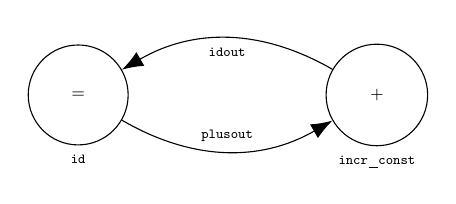
\begin{tikzpicture}[font=\tiny,
      proc style/.style={circle,draw=black,align=center,text
        width=1cm,minimum size=1cm,align=center}
      ]
      \node[proc style] (id) {$=$};
      \node[below=0cm of id] (p1) {{\ttfamily id}};
      \node[proc style,right=2.5cm of id] (add) {$+$};
      \node[below=0cm of add] (p2) {{\ttfamily incr\_const}};
      \draw[-{Latex[scale=1.6]}] (id) edge [bend right=30] node [above] {{\ttfamily plusout}} (add);
      \draw[-{Latex[scale=1.6]}] (add) edge [bend right=30] node [below] {{\ttfamily
          idout}}
      (id);
    \end{tikzpicture}
    }
    \caption{A simple SME network consisting of two processes. One simply
      forwards the received value while the other increments it by a
      constant. The names of the processes and buses corresponds with the names
      in \Cref{fig:addone.sme}}
  \label{fig:addone}
\end{figure}
\begin{widefigure}
\begin{smeilcode2}
proc id(in inbus)
  bus idout {
    val: int;
  };
  var it: uint = 0;
{
  idout.val = inbus.val;
  trace("Iteration: {} Value: {}",
    inbus.val, it);
  it = it + 1;

}



proc incr_const(in inbus, const val)
  bus plusout {
     val: int;
  };
{
  plusout.val = inbus.val + val;
}

network incr() {
  instance plusone_inst of
    plusone(id_inst.idout, val: 10);
  instance id_inst of
    id(plusone_inst.plusout);
}
\end{smeilcode2}
\caption{An example program written in SMEIL.}
\label{fig:addone.sme}
\end{widefigure}

Before closing this chapter, let us show an example of a small, but complete
example of an SME network implemented in SMEIL to give a feel of the language
and show how everything fit together. The \textsc{addone} network,
illustrated in \Cref{fig:addone} to give a feel of the language and illustrate
the basic syntax. The network consists of two processes and two buses. One
process, labeled ``='' simply passes along the value received while the other
process increments it by a constant value passed as a parameter. The source code
for the example is shown in \Cref{fig:addone.sme}.

Each of the two processes is declared using a {\ttfamily proc} block. Immediately
following, are the declarations belonging to the processes. In this case, both
of the processes declares the bus used for sending their output values. Both
processes are also parameterized by a bus on which they receive their input
values. The {\ttfamily incr\_const} process takes an additional parameter which is a
constant value added to the input value. The curly-braces in a process contain
the statements constituting its procedural parts, that is, the actions that are
performed when the process is executed during a clock cycle. The network {\ttfamily
  incr} instantiates the two processes and connects the output one to the input
of the other. Furthermore, for the instance {\ttfamily plusone\_inst} the constant
{\ttfamily val} parameter is also set, making the {\ttfamily incr\_const} process 1add 10 to
the value it receives every time its run. Declarations may be given in any
order, allowing the mutually dependent process instantiations in the {\ttfamily incr}
network.






% \subsection{Type checking}
% An entire program, including all modules is type checked from the top down,
% meaning that the outer leafs of the import tree is type checked first. The outer
% leaves of a modules should be self-contained

% \subsection{Modules}
% It is possible to split SME networks across several modules for program
% structuring and separation of purpose.  Both the module system and the syntax
% used for importing modules are similar to the system used by the Python
% programming language: A file constitutes a module, carrying the name of the
% file. Module hierarchies are created through folders. Unlike Python, we have no
% default file-name allowing a folder to be imported as a module. Each program
% must define a \textit{top level network} which is used as the starting point of
% \textsc{network} exploration during compilation. A top level network is a
% \textsc{network} that has the same name as the module (file) it is defined in)
% Let us look at some examples showing how module hierarchies are created and
% imported.

% \subsection{Importing process}


% The performance of this part of the compiler is assumed to be abysmal due to the
% multiple syntax tree traversals using slow type-generic traversal mechanisms.

% \begin{enumerate}
% \item A module is parsed and any parsing errors are reported
% \item We extract a list of imports 
% \end{enumerate}

% \subsection{Instances}
% \label{sec:instnaces}
% Processes and networks (together called \textit{entities}) can be
% \textit{instantiated} in other networks. When declaring an instance of an
% entity, we can set entity parameters (input- and output buses or
% constants). Declaring an instance makes a instance-private copy of all fields
% declared in the entity. For buses, this behavior may be undesired in cases a
% single bus should be connected to multiple inputs and we therefore provide the
% \texttt{unique} declaration modifier for buses.\fxnote{Example}. The buses
% declared within a process may be referred to through their
% instances. Alternatively, buses may be referenced through the declared name of
% their encapsulating entity. In this case, the instance referenced is the
% \textit{default instance} of which one exists for every instance.

% \section{Compiling SME programs}
% The transformation and processing of SME programs is performed in a series of
% steps gradually transforming the source code into the intended format is
% reached. We describe these steps and the reason for their existence in this
% section.

% \paragraph{Program normalization through module flattening.} The very first step
% of the compilation process seeks to simplify subsequent compilation passes by
% flattening the hierarchy of included modules. This step also parses all
% dependencies of a program. A module import is handled through recursive
% descendant evaluation of imports where different information is passed on the
% outgoing and incoming edges of the module dependency graph. On the outgoing
% edges, we pass the import ``paramteres'' of a module and on the incoming edges
% we pass the renamed module. Every time something is passed on an incoming edge,
% it is folded (merge) into the code on that level. Before merging, all top-level
% names and references to those names are renamed such that there is no
% name-clashes with the code that the module is being merged into. During this
% process, we also ensure that all imported names actually exists and produce a
% error if they do not.

% \paragraph{Type checking}
% Doing immediate type checking may not be desireable given our goal of being able
% to assign types rather late. On the other hand, we want to generate 

% A key assumption in performing TypeChecking of SME programs is that buses are
% the only entities that are cross-referenced between processes and
% networks. Therefore, we can do type checking as a two-pass process where we
% first iterate through all defined top-level entities and add their buses to the
% type checking environment.

% Type checking happens through several symbol tables. One per scope. We have one
% (global) symbol table per program and a local table for each entity. Before
% type checking is started, all the static declarations of each scope has already
% been filled out. The per-entity symbol table have a global and a local
% part. Lookups into global symbols may transcend the current scope, thus
% accessing the scope of another entity. Lookups may be implemented in one of two
% ways. Either we merge parent tables before we enter an entity, meanining that we
% only need to query into asingle symbol table. Alternatively we may allow
% recursive lookups such that the global scope is tried once the name is
% non-existing in the inner scope.

% For deciding function parameters we need to maintain a history of which
% parameters a function as been instantiated with. This will allow us to decide if
% a) all of the buses used have the same type and b) the bounds of constants for
% type checking purposes.


% \section{Converting to VHDL}

%%% Local Variables:
%%% mode: latex
%%% TeX-master: "../master"
%%% TeX-command-extra-options: "-enable-write18"
%%% End:

\chapter{Co-simulation}
\label{sec:cosim}

% Without a method for providing external input to SME networks  would not be very
% useful.
The usefulness of SMEIL would be limited without a way to provide external
interactions with SME networks written in SMEIL. The simplicity of SMEIL can be
attributed to its narrow scope: it is only intended for writing hardware models
and not for writing test benches. For this, the full power of a general-purpose
language is needed as the test-code can be written without hardware-related
considerations and using all available libraries. For example, a test bench may
read an image from disk or visualize the results of a simulation. Extending
SMEIL to be able to perform such tasks is a substantial undertaking that does
not further its primary purpose as a hardware-modeling
language. Co-simulation~\cite{schloegl2015towards} is the process of two
separate entities (in this case two SME networks) which communicates through
channels transparently established by the SME libraries.

\section{Co-simulation with SMEIL}
For performing co-simulation with SMEIL, we expose a C API from \libsme{}. The
API is intended to be implemented by SME libraries for general-purpose
languages.

There are three aspects to the API: Firstly it provides a way to enumerate the
buses exposed from a SMEIL model. Secondly, it provides calls for reading to-
and writing from bus channels and driving forward the simulation. Finally, it
offers calls for ordering the production of output, such as VHDL code
generation.

A noticeable feature of the API is its support for arbitrary-length
integers. This means that the bit-width of buses used by simulated models are
not restricted by the register-width of the CPU of the underlying host. A
hardware model may use values of any bit-width and the model should, therefore,
not inherit the limitations of the platform that it is simulated on.

% Support for
% simulating designs using integers larger than the register-width of the host CPU
% is desired since it allows them to be used in hardware models. \todo{fix}

When the co-simulation API is used \libsme{} operates as a ``puppet'', being
controlled by the calling program (the ``puppeteer''). Only buses declared with
the \texttt{exposed} (\Cref{sec:langref}) modifier in SMEIL are accessible
through the \libsme{} API. The calling library drives forward the simulation by
calling a function for ticking the clock and for reading and writing from/to the
exposed buses of a SMEIL program. In the following section, we give a detailed
introduction to the API.  For brevity, we refer to an SME library implementing
the API as the ``client'' in the following.

% \begin{figure}
%   \resizebox{.7\linewidth}{!}{
%     \begin{tikzpicture}[>=latex]
%       \coordinate (A) at (2,5);
%       \coordinate (B) at (2,0);
%       \coordinate (C) at (6,5);
%       \coordinate (D) at (6,0);

%       \draw[thick] (A)--(B) (C)--(D);

%       \draw (A) node[above]{libsme};
%       \draw (C) node[above]{Client};

%       \coordinate (E) at ($(A)!.25!(B)$);
%       \coordinate (F) at ($(C)!.1!(D)$);
%       \draw[->] (F) -- (E);
%     \end{tikzpicture}}
% \end{figure}


The approach presented here is conceptually similar to the Verilog Procedural
Interface (VPI)~\cite{dawson1996verilog} which is used for interfacing with
Verilog and VHDL simulators. However, a big advantage of the SMEIL approach is
that SME is used on both sides of the co-simulation. Hence, both the functional
and verification parts of the network act as a single unified entity. Thus, the
programmer does not need to consider integrating different abstract interfaces.


\section{API reference}
This section documents the public API of the co-simulation interface of
\libsme{}. Towards the end of the section, we give a short overview of how the
API is used.

\subsection{Exported data structures}
\begin{lstlisting}[language=c,multicols=2]
typedef enum Type {
  SME_INT,
  SME_UINT,
  SME_FLOAT,
  SME_DOUBLE,
  SME_BOOL
} Type;

typedef struct SMEInt {
  int len;
  int alloc_size;
  int negative;
  char* num;
} SMEInt;

typedef struct Value {
  Type type;
  union {
    bool boolean;
    SMEInt* integer;
    double f64;
    float f32;
  } value;
} Value;

typedef struct ChannelRef {
  char* bus_name;
  char* chan_name;
  Type type;
  Value* read_ptr;
  Value* write_ptr;
} ChannelRef;

typedef struct BusMap {
  int len;
  ChannelRef** chans;
} BusMap;
\end{lstlisting}

The data structures listed above constitute the primary interface for exchanging
data with \libsme{}.

\subsection{Public API}
\begin{description}
\item[\texttt{SmeCtx* sme\_init()}]\hfill\\
   Initializes and returns the SME library context.
 \item[\texttt{bool sme_open_file(SmeCtx* ctx, const char* file, int argv,
     char** argc)}]\hfill Loads an SMEIL file, while applying the supplied
   arguments to \libsme{}.
   \item[\texttt{bool sme_has_failed(SmeCtx* ctx)}]\hfill\\
     Returns true if an operation within the \libsme{} library failed.
 \item[\texttt{char* sme_get_error_buffer(SmeCtx* ctx)}]\hfill\\
   Returns a string containing the error message emitted by \libsme{}. The memory
   pointed to may not be freed except by calling the \texttt{sme_free} function.
 \item[\texttt{void sme_free(SmeCtx* ctx)}]\hfill\\
   Frees the SME library context and related resources.
 \item[\texttt{bool sme_tick(SmeCtx* ctx)}]\hfill\\
   Ticks the clock of an SME simulation synchronously. When this function
   returns, all processes defined within \libsme{} will have run and written to
   their buses.
 \item[\texttt{bool sme_finalize(SmeCtx* ctx)}]\hfill\\
   Finalizes a simulation and dumps the recorded trace file (if any) to the file
   system. This function should always be called following the final call to
   \texttt{sme_tick}.
 \item[\texttt{bool sme_propagate(SmeCtx* ctx)}]\hfill\\
   Propagates the values of both internal and external facing buses defined in
   \libsme{}. Run this function before the clock is advanced (by calling
   \texttt{sme_tick}) in the simulation loop and it should be run together with
   any bus propagation that needs to be performed by the calling code. When this
   function returns, the values of all buses defined within \libsme{} have been
   propagated.
 \item[\texttt{void sme_integer_resize(SMEInt* num, int len)}]\hfill\\
   When manipulating values of type {\tt SMEInt} (arbitrary-size integers) the
   \texttt{sme_resize_integer} function will make sure that the memory pointed
   to by {\tt Value.value} is large enough to hold the number that you intend to
   store. The function takes a pointer to the {\tt SMEInt} structure and a
   parameter len which is the number of bytes needed to store the number as
   base-256. This function must be called before every direct manipulation of
   {\tt SMEInt.num}. For a safer interface, see \texttt{sme_integer_store}.
 \item[\texttt{void sme_integer_store(SMEInt* num, int len, const char val[])}]\hfill\\
   Stores the base-256 representation of an integer in an \texttt{SMEInt}.
 \item[\texttt{void sme_set_sign(SMEInt* num, int sign)}]\hfill\\
   Sets the sign of an \texttt{SMEInt}. Possible values for \texttt{sign} are 0
   meaning the number is positive and 1 for a negative value.
 \item[\texttt{BusMap* sme_get_busmap(SmeCtx* ctx)}]\hfill\\
   Returns a pointer to a {\tt BusMap} structure containing the exposed buses of
   the SME network. This function is intended to be used by implementers of
   \libsme{} to generate internal representations of their SME buses. It is the
   callers responsibility to free the memory returned by the function by calling
   \texttt{sme_free_busmap}.
\item[\texttt{void sme_free_busmap(BusMap* bm)}]\hfill\\
   Frees a BusMap structure allocated by \texttt{sme_get_busmap}.
\end{description}

\subsection{Using the API}
The initial interaction with the API happens through a call to the {\tt
  sme_init} function. The {\tt SmeCtx} pointer returned is an opaque reference
to the SME library context which must be included in every future interaction
with the library. The next step is to load a SMEIL program by calling {\tt
  sme_open_file}. Then, the implementing client must retrieve a {\it busmap}
from \libsme{} in order to learn how to access the {\tt exposed} buses of the
SMEIL program. This is done by calling the {\tt sme_get_busmap} function. As
seen, it returns a pointer to a {\tt BusMap} struct which then again points to
an array of {\tt ChannelRef} structs. Each of these contains an individual bus
channel. In addition to the type of the channel, a {\tt ChannelRef} also
contains two pointers to {\tt Value} structs. One for the reading- and
writing-end of the channel respectively. Reading to- and writing from the bus
channel is done by directly accessing these {\tt Value}s. A {\tt Value} consists
of the actual value plus its type. The only value which is not simply
represented using a native C type is {\tt SMEInt} which, as seen, contains a
{\tt char*}. This is a pointer to the memory used for storing the individual
bytes of a base-256 integer. Before this memory is written, the {\tt
  sme_integer_resize} function must be called to ensure that the memory is large
enough to contain the number that the client intends to store.

After each of these calls, the {\tt sme_has_failed} must be called in order to
check if the previous operation resulted in an error. If the function returns
{\tt true}, the {\tt sme_get_error_buffer} function returns a pointer to a
buffer containing a human-readable description of the error which occurred.

In the main simulation loop of the implementing client library the following
calls to the API are usually made: In the bus propagation phase, the client must
propagate its own buses and then call the {\tt sme_propagate} function to
propagate the buses defined the SMEIL program. Following bus propagation, the
client library must run its own processes and the processes defined in the SMEIL
program. The processes defined in the SMEIL program are run by calling the {\tt
  sme_tick} function.

When the simulation is complete and the desired number of cycles has been
performed, before freeing memory, a final call to {\tt sme_finalize} must be
issued in order to dump the recorded trace file to disk.

The intention of this API is that it should be as general as possible such that
it can be implemented by any language providing an adequate Foreign Function
Interface (FFI) for C APIs.

\section{Co-simulation using PySME}

\begin{figure}
  \centerfloat
  \begin{subfigure}[t]{0.40\paperwidth}
\begin{lstlisting}[language=smeil]
proc addone(in inbus, const val)
    exposed bus addout {
       val: i32;
    };
{
    addout.val = inbus.val + val;
}

network addone_net() {
    exposed bus idout {
        valid: bool;
        val: i32;
    };

    instance addone_inst of
        addone(idout, 1);
}
\end{lstlisting}
    
\subcaption{The SMEIL code in \texttt{addone.sme}.}
  \end{subfigure}
  \begin{subfigure}[t]{0.40\paperwidth}
    \begin{lstlisting}[language=python]
from sme import *

class Id(SimulationProcess):
  def setup(self, ins, outs, result):
    self.map_outs(outs, "out")
    self.map_ins(ins, "inp")

  def run(self):
    result[0] = self.out["val"]
    self.out["val"] = self.inp["val"]

@extends("addone.sme", ["-t", "trace.csv"])
class AddOne(Network):
  def wire(self, result):
    plus_out = ExternalBus("addone_inst.addout")
    id_out = ExternalBus("idout")
    p = Id("Id", [plus_out],
      [id_out], result)
    self.add(plus_out)
    self.add(id_out)
    self.add(p)

if __name__ == "__main__":
  sme = SME()
  result = [0]
  sme.network = AddOne("", "AddOne",
             result)
  sme.network.clock(100)
  print("Final result was ", result[0])
  \end{lstlisting}
  \subcaption{The corresponding Python code.}
  \end{subfigure}

  \caption{Example code showing the an interaction between SMEIL (left) and PySME
    (right).}
\label{fig:smeilpy}
\end{figure}

In order to show a client implementation of the API described above, we have
extended the PySME library~\cite{pysme} with support for co-simulation enabling
seamless interaction between SME networks written in Python and SMEIL. In
practice, extending the PySME library was straightforward and required less than
a day of implementation work by a person with expert knowledge of both
code-bases. We expect that a similar effort is required to extend other SME
implementations (such as C\# SME and C++ SME).

As an example, we revisit the {\sc addone} example introduced in \Cref{sec:smeilex},
this time implementing one half of it in Python as seen in
\Cref{fig:smeilpy}. The \texttt{@extends} decorator is all that is needed to
make the buses exposed from the SMEIL network available for the Python
program. Behind the scenes, \libsme{} is loaded and the \texttt{addone.sme} file
is parsed, typechecked and the \libsme{} SMEIL simulator is initialized. We gave
a detailed description of this interaction in the previous section. A
SMEIL-defined bus is referenced from PySME by instantiating an
\texttt{ExternalBus}, providing the name of a bus defined in the SMEIL program
as its parameter. The semantics of an {\ttfamily ExternalBus} is identical to
those of a bus defined within Python. Any SMEIL type except strings and arrays
may be passed along a bus. Strings play a very limited role in SMEIL and are
therefore unlikely to be supported. Arrays, on the other hand, are desirable to
include in future extensions. Integers are encoded in base-256 as a sequence of
bytes, allowing arbitrarily-sized integers to be used between co-simulated
entities.

When this program is run, the PySME library calls the \libsme{} library for
every cycle to stepwise progress the simulation. During the simulation \libsme{}
may, if asked to do so, record a trace of the communication taking place over
the buses to a file. This trace file is then later used as the data source for
the VHDL test bench which is used to verify the generated VHDL code.

This is a highly flexible model as co-simulation is enabled with minimal
intrusion on existing PySME code. For example, should \libsme{} be extended with
a high-performance simulation backend for SMEIL, existing programs can take
advantage of this without modifications. The implementation of \libsme{} may
even be replaced entirely, as long as the current API is
maintained. Furthermore, it also facilitates an incremental design strategy,
where a Python prototype can gradually be rewritten in SMEIL.

Notice in the PySME code of \Cref{fig:smeilpy} that the {\tt addout} bus is
referenced through its instance name {\tt addone_inst.addout} and the {\tt
  idout} bus is referenced directly by its name. This is because the latter bus
is declared directly inside the top-level entity while the former is declared
within the {\tt addone} process which is instantiated as {\tt addone_inst}.
This naming scheme is used to ensure that exposed buses have unique names.

We show more examples of using co-simulation for testing SMEIL networks in
\Cref{eval}.

% \section{Runtime representation}
% In order to perform a simulation of  SMEIL network, we transform it to a
% suitable runtime representation. 


\section{Typing networks through simulation}
\label{sec:typing}
% \todo{Why do we only have this restricted notion of dynamic typing. Why no
% completely variable types?}
As described in \Cref{sec:typesys} SMEIL supports integers of both constrained
and unconstrained bit-widths.  In order to translate SMEIL to a hardware
description, we require that all types in the program are constrained to a
specific bit-width.  In a hardware description, we need to statically specify
the number of bits required by each value and therefore, arbitrary-width
integers are not representable.  However, it is often difficult to decide the
optimal bit-width of a value in advance. In particular, this applies to internal
variables whose values are derived from external inputs. To address this,
\libsme{} provides a method for re-typing a SMEIL program based on values
observed during simulation.

When this feature is enabled, the maximum absolute value assigned to a variable
is stored alongside its current value. Whenever the variable is assigned, the
new value is compared to the current maximum which is then updated as needed.

% As described in \Cref{sec:typesys}, the only unsized types which exists in SMEIL
% are signed and unsigned integers. This raise the question: Why not have an
% {\ttfamily any}-type which could unify with any other type? A related form of
% the question is: Why distinguish between signed and unsigned unsized integer
% when the signed type is the superset of the two

%\todo{Describe implementation details}
%\todo{We promise to mention ranges earlier}
When the simulation is concluded, the observed value ranges are converted to
SMEIL types large enough to hold the range.  For example, in the program shown
in \Cref{fig:non-violated}, we observed that the bus channel {\tt b.chan} was
assigned values between 0 and 29 during simulation. Therefore, the bus channel
is assigned the type {\tt i6} as we need 6-bits to hold the value 29 in a signed
integer.

The types and observed ranges are spliced into the SMEIL AST and the re-typed
program is then passed through the type checker. This ensures that constraints
originating from fixed-size types in the original program are not violated. This
process is illustrated in \Cref{fig:simtyping} which shows how observationally
derived types are spliced into an existing program. \Cref{fig:violated} shows
the violation of an existing constraint in the program. Since the value
{\ttfamily c} has the fixed-sized type {\ttfamily i10}, the program will no
longer be valid if {\ttfamily b.chan} observes values that are 16-bit long. A
configuration flag {\ttfamily -{}-no-strict-type-bounds} overrides this behavior
by considering all types as unconstrained (i.e., {\ttfamily i10} is considered
identical to {\ttfamily int}).


\begin{widefigure}
  \centering
  \begin{subfigure}[t]{0.30\linewidth}
    %\centering
\begin{lstlisting}[language=smeil]
proc A ()
 bus b {
  chan: ?{\bfseries\underline{int}}?;
 };
 var c: i10;
{
 c = b.chan;
}
\end{lstlisting}
    \caption{Unconstrained types.}
    \label{fig:oktype}
  \end{subfigure}
  \begin{subfigure}[t]{0.30\linewidth}
    %\centering
    \begin{lstlisting}[language=smeil]
proc A ()
 bus b {
  chan: ?{\bfseries\underline{i6 range 0 to 29}}?;
 };
 var c: i10;
{
 c = b.chan;
}
    \end{lstlisting}
    \caption{Valid.}
    \label{fig:non-violated}
  \end{subfigure}
  \begin{subfigure}[t]{0.30\linewidth}
    %\centering
    \begin{lstlisting}[language=smeil]
proc A ()
 bus b {
  chan: ?{\bfseries\underline{i16 range 0 to 30717}}?;
 };
 var c: i10;
{
 c = b.chan;
}
\end{lstlisting}
    \caption{Invalid.}
    \label{fig:violated}
  \end{subfigure}
  \caption{Shows a process entering the simulator with an unconstrained type (a)
    and examples of two possible resulting programs (b, c). The type changing
    between the examples is underlined.}
  \label{fig:simtyping}
\end{widefigure}

As seen, it is possible to mix types with constrained and unconstrained
bit-widths, This is useful as we often know the possible range of external
buses. Determining the ranges of values that derive from those buses are not
always as easy. Therefore, we can let all internal buses and variables of a
program be typed based on observed values while fixing external buses to a
specific size. The type system of SMEIL will then enforce that we do not assign
a larger dynamically determined value to a smaller fixed external value.
% Facilities for
% bit-precise typing also exists in other current SME implementations, but since
% the types aren't built into the language, they become more difficult to enforce

This feature can only be used safely if the following conditions
apply: \begin{inparaenum}[1)] \item All values deriving from input stimuli must
  increase monotonically in relation to the value of the input and \item the
  testing code must ensure that the whole possible range of input stimuli is
  exhausted by test benches.
\end{inparaenum}

To allow easy examination of the types derived from value observations without
having to examine the generated source code, \libsme{} is able to display the
SMEIL program with the modified types in place. That is if the program shown in
\Cref{fig:oktype} was simulated, the resulting code shown in
\Cref{fig:non-violated} or \Cref{fig:violated} would be what is actually shown
to the user.

% A limitation of the current implementation is that SMEIL buses are referenced by
% their bare name, rather than in relation to their position in the instance
% hierarchy. In SMEIL, it is perfectly valid to have multiple buses by the same
% name as long as are not declared in the same scope. However, having several
% {\ttfamily exposed} buses by the same name and referencing them through the
% co-simulation API currently results in undefined behavior. \libsme{} should be
% modified to either disallow multiple {\ttfamily exposed} buses globally, or
% better, to export buses through the API using hierarchical names. The latter is
% already being done by the VHDL code generator.
% \todo{This is not quite correct}

\section{Alternative approaches}
We considered a couple of alternative approaches before settling on this final
design. As written in the introduction to this chapter, co-simulation was
introduced as a method for providing external test inputs to SMEIL programs.
Instead of adding the API for performing co-simulation, we could simply require
that all SMEIL programs expecting external inputs would take these inputs from a
\gls{csv} trace-file generated by simulating an equivalent SME network. In this
scenario, the starting point would be a complete SME network implemented in, for
example, PySME. Simulating this network would generate a trace-file containing a
recording of values sent over buses. Then, the hardware-targeted processes of
the PySME model would be translated to SMEIL and the recorded trace-file would
be used for providing input to the SMIEL model.

%\todo{Why would this be a problem?}
Implementing this model would require less work, but it would only support using
SMEIL as an intermediate language. The reason for this is the following: in
order to generate the required trace file, a complete implementation of the SME
network in a single language is required, thus, it would not be possible to
implement a part of the network separately in SMEIL. Furthermore. the
co-simulation model delegates the responsibility of generating the trace-file to
\libsme{}. Since \libsme{} is also responsible for generating the final VHDL
code, this makes it simpler to ensure that names and order of fields in the CSV
file match those expected by the generated VHDL test bench. If the trace file
was generated externally, it would also prevent changing the \libsme{}
implementation in a way which altered the naming and ordering of fields in the
CSV files. Thus, the co-simulation model is advantageous even when SMEIL is used
as an \gls{il}, and without it, SMEIL would not be usable as a primary
implementation language at all.

\paragraph{External library generation.}
Insetad of implementing an interface to the simulator within \libsme{}, we
considered the alternative approach of generating an external library (for
example in C++) and expose an API similar to the current. However, instead of
loading the \libsme{} library and asking it to load an SMEIL program, we would
load the generated library directly. The advantages of this would be:
\begin{enumerate}
\item We would get two birds with one stone by both providing a method for
  co-simulation and a C++ code generator.
\item The SMEIL code would be compiled to native code and therefore execute
  significantly faster.
\item A library generated from a SMEIL program would be significantly smaller
  than all of \libsme{} and could be distributed independently.
\end{enumerate}
However, the disadvantages would be:
\begin{enumerate}
\item More complex client library integration: A library performing
  co-simulation with SMEIL would first need to compile the SMEIL code to a
  library, then load the library. We could handle this from \libsme{}, but that
  would diminish the third advantage.
\item The implementation of observationally-derived typing (\Cref{sec:typing})
  would become more complicated as the observed types would need to be
  communicated back to \libsme{} in order for them to be used in the code
  generated from the SMEIL program.
\end{enumerate}
    
\paragraph{API considerations.}
The second consideration made was how to actually expose the API. As an
alternative to the current C API, a web-based REST-style API was also
considered. To implement this, \libsme{} would contain a web-server which would
listen to requests from a client library. The advantage of this approach would
be that web-APIs are more ubiquitous that C-style APIs, and thus, they may be
able to support a wider range of clients. On the other hand, we were concerned
with the performance of such an approach as issuing an HTTP request carries a
significantly higher overhead than performing a platform level C-call. Another
concern with the currently chosen approach was whether it was sufficiently
platform-neutral. However, we feel reasonably confident that the current
approach is supported on all major platforms, although only Linux has been
tested.


%%% Local Variables:
%%% mode: latex
%%% TeX-master: "../master"
%%% End:

\chapter{Code Generation}
\label{sec:codegen}
SMEIL compiles to clean and readable VHDL code which is amenable to manual
modifications, should this be desired. The code may be executed using a VHDL
simulator or passed to FPGA vendor tools for synthesis and subsequent
hardware-implementation. The generated code is a cycle-accurate representation
of the original SMEIL network.
\todo{Make more detailed or don't use a separate chapter.?}

\section{Naming in VHDL}
A key issue is how to handle the transformation of names when moving from
transforming an SMEIL program to VHDL. Since an entity in an SMEIL program
translates directly to a VHDL entity, we need to make sure that names in the
original SMEIL program remains unique
\todo{Show example from EWMA top-level entity}

\section{Code transformations}
%In the f

The fundamental structure of the SMEIL code is preserved in the generated
VHDL. One VHDL entity is generated per SMEIL entity and the body a SME process
is transformed to a sequential process in VHDL. For each of these processes, we
also generate code for performing an asynchronous reset of all variables and
outgoing signals. The naming hierarchy of the original SMEIL is preserved,
making it easy to identify from where a particular section of the VHDL code was
generated.

For verifying the generated VHDL code, a test-bench is also generated. The
test-bench is a VHDL program which connects to the {\ttfamily exposed} buses of
the SMEIL program. The CSV-trace file containing the values recorded during
simulation is used by the VHDL test bench to drive inputs and verify outputs.

Alongside the generated code, a {\ttfamily Makefile} is generated for building
and testing the VHDL code using the GHDL~\cite{ghdl} simulator.

Integer types of SMEIL are represented in VHDL using the types provided by the
standard {\ttfamily ieee.numeric\_std} package. This package provides functions for
performing signed and unsigned integer arithmetic with logic-vectors. For
example, the types {\ttfamily i4} and {\ttfamily u12} are represented as {\ttfamily signed (3
  downto 0)} and {\ttfamily unsigned (11 downto 0)} respectively. Arrays require the
creation of a new {\ttfamily type} in VHDL. A {\ttfamily type} declaring a 10-element array
of 5-bit signed integers ({\ttfamily [10]i5} in SMEIL) is represented in VHDL as
\begin{lstlisting}[language=vhdl]
type \[10]i5\ is array (0 to 9) of unsigned (4 downto 0);
\end{lstlisting}
These type declarations are stored in a separate package, {\ttfamily sme\_types.vhdl},
which is shared between all entities of the design to avoid cluttering the
generated code with duplicated declarations. SMEIL booleans are represented
using the VHDL type {\ttfamily boolean}. As an alternative to this, a single {\ttfamily
  std\_logic} type is commonly used. This type represents a wire in the hardware
and is, therefore, able to have other states than just true or false. This may
be useful in some circumstances.

The actual code is generated using the {\ttfamily language-vhdl-quote}
library~\cite{language-vhdl-quote} which provides
quasiquoters~\cite{mainland2007s} for building VHDL ASTs using the concrete VHDL
syntax. The major advantage of this approach is that it minimizes the chance of
generating syntactically invalid VHDL since syntax errors are caught during
compilation of \libsme{}. Furthermore, a complete VHDL AST is constructed
containing the contents of each generated VHDL file. This AST is then
pretty-printed, yeilding consistently formatted code which is difficult to
achieve using more common techniques using string-based templates.


%%% Local Variables:
%%% mode: latex
%%% TeX-master: "../master"
%%% End:

\chapter{\libsme{} design and implementation}

In this section, we present the combined implementation of \libsme{} and
elaborate on implementation details.

\section{Methods of interaction}
\label{sec:using}
SMEIL programs are run using the {\ttfamily libsme} library either through interaction
with the C API of the library or by using the provided command line utility.

\begin{description}
\item[Direct code generation.]
  % A SMEIL program constitutes a complete
  % description by itself provided that only size constrained types are
  % used.
  A SMEIL program that contains only size-constrained types provide all the
  information that is needed to generate a hardware description. Therefore, VHDL
  code can be generated directly from a SMEIL program without the intermediate
  simulation step. Some advantages are lost when using this mode, as no test
  bench is created and the generated VHDL code must be manually modified and
  connected to a clock source for driving the simulation before it can be tested
  using a VHDL simulator.
\item[Pure SMEIL simulation.] This mode only applies to SMEIL networks which
  contain their own data generation process (see \Cref{sec:7seg} and
  \Cref{sec:md5} for examples of such networks). SMEIL used like this is not
  very useful as it can only produce an output through {\ttfamily trace}
  statements (\Cref{sec:langref}).
\item[Co-simulation of SMEIL.] The most common intended usage scenario for SMEIL
  is to use it together with an SME library for a general purpose language. This
  allows the generation of VHDL code, an associated test bench, and a trace
  file. The full details of the co-simulation interface of SMEIL were previously
  given in \Cref{sec:cosim}.
\end{description}

\label{sec:libsmeimpl}
\begin{figure}%[tb]
  \centering
  \resizebox{\linewidth}{!}{
    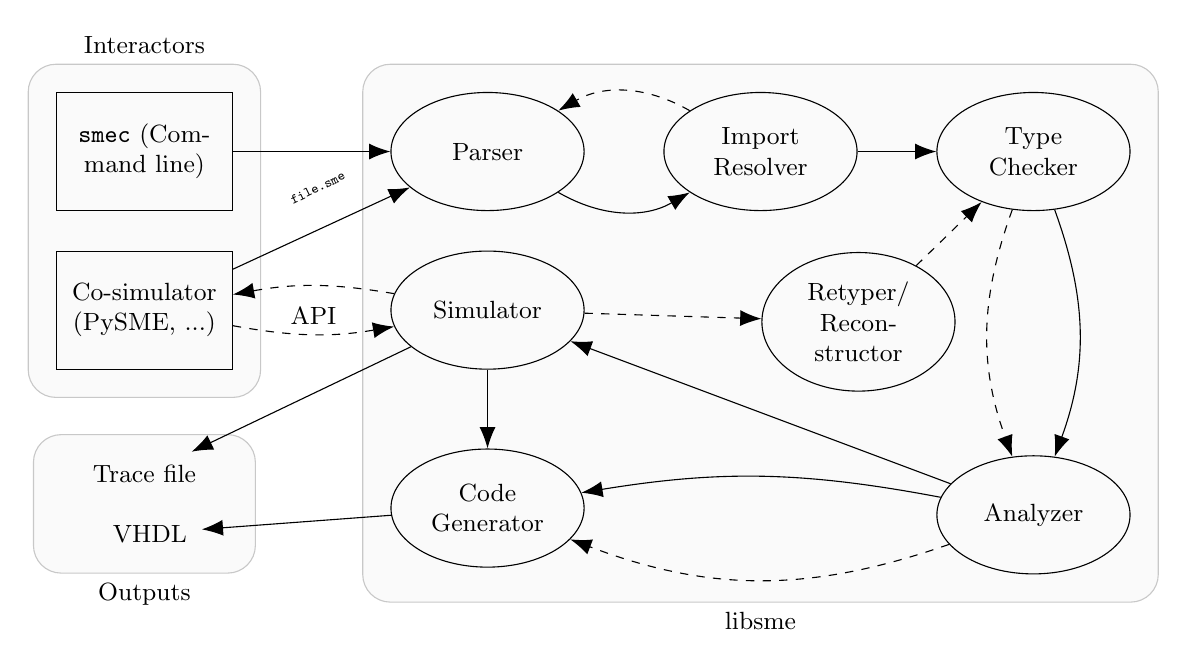
\begin{tikzpicture}[font=\small,
      rep style/.style={rectangle,draw=black,text width=1.5cm,minimum
        size=1.5cm,align=center},
      proc style/.style={ellipse,draw=black,align=center,text
        width=1.5cm,minimum size=1.5cm,align=center},
      file style/.style={ellipse,draw=none,align=center,text
        width=1.5cm,minimum size=0.5cm,align=center}
      ]
      \node[proc style] (parser) {Parser};
      \node[proc style, right=1cm of parser] (import) {Import Resolver};
      \draw[-{Latex[scale=1.6]}] (parser) edge [bend right=30] (import);
      \draw[-{Latex[scale=1.6]},dashed] (import) edge [bend right=30] (parser);

      \node[proc style, right=1cm of import] (tyc) {Type Checker};
      \draw[-{Latex[scale=1.6]}] (import) edge (tyc);
      \node[proc style, below=3.1cm of tyc] (an) {Analyzer};

      \draw[-{Latex[scale=1.6]}] (tyc) edge [bend left=20] (an);
      \draw[-{Latex[scale=1.6]},dashed] (tyc) edge [bend right=20] (an);

      \node[proc style, below right=1cm and -0.5cm of import] (recon) {Retyper/\\Recon-\\structor};
      \node[proc style, below=0.5cm of parser] (sim) {Simulator};
      \node[proc style, below=1cm of sim] (codegen) {Code Generator};
      \draw[-{Latex[scale=1.6]}] (an) edge (sim);

      \draw[-{Latex[scale=1.6]}] (sim) edge (codegen);
      \draw[-{Latex[scale=1.6]},dashed] (sim) edge (recon);
      \draw[-{Latex[scale=1.6]},dashed] (recon) edge (tyc);
      \draw[-{Latex[scale=1.6]},dashed] (an) edge [bend left=20] (codegen);
      \draw[-{Latex[scale=1.6]}] (an) edge [bend right=10] (codegen);

      \node[rep style, left=2cm of parser, text width=2cm] (cmdl)  {{\ttfamily  smec} (Command line)};

      \node[rep style, below=0.5cm of cmdl, text width=2cm] (cosim)  {Co-simulator\\(PySME, ...)};
      \draw[-{Latex[scale=1.6]},dashed] (cosim) edge [bend right=10] node[above] {API} (sim);
      \draw[-{Latex[scale=1.6]},dashed] (sim) edge [bend right=10] (cosim);
      \draw[-{Latex[scale=1.6]}] (cosim) edge  (parser);

      \draw[-{Latex[scale=1.6]}] (cmdl) edge node[below=0.3cm,rotate=26]
      {{\ttfamily \tiny file.sme}} (parser);

      \node[file style, below=1cm of cosim] (trace) {Trace file};
      \node[file style, below=0.1cm of trace, text width=0.8cm] (vhdl) {VHDL};

      \draw[-{Latex[scale=1.6]}] (sim) edge (trace);
      \draw[-{Latex[scale=1.6]}] (codegen) edge (vhdl);

      \begin{scope}[on background layer]
        \node[draw=scopeborder,fill=scopebg,inner sep=10pt,rounded corners=10pt,anchor=north west,fit=(parser)(an)(codegen),label={below}:libsme] (libsme) {};
        \node[draw=scopeborder,fill=scopebg,inner sep=10pt,rounded corners=10pt,anchor=north west,fit=(cmdl)(cosim),label={above}:Interactors] (inter) {};
        \node[draw=scopeborder,fill=scopebg,inner sep=5pt,rounded corners=10pt,anchor=north west,fit=(trace)(vhdl),label={below}:Outputs] (inter) {};
      \end{scope}
    \end{tikzpicture}
  }
  \caption{Overviews of interactions with and data flow within \libsme{}. The
    dashed lines denotes paths which are followed conditionally depending on
    which mode \libsme{} is executed in.}
  \label{fig:overview}
\end{figure}

\section{An overview}
\label{sec:overview}
In the previous sections, we have described the individual parts of \libsme{}
without describing the integration of its components. Hence, we devote a section
for that purpose here. An overview of the \libsme{} library and its interactions
is shown in \Cref{fig:overview} and the individual stages are described below.

\subsection{Parsing and Import Resolution} Regardless of how \libsme{} is
invoked (as described in the previous section) the SMEIL source is parsed and
the resulting AST is passed through the import resolver. Here, the code is
scanned for the presence of {\ttfamily import} statements. If any are found, the source
files containing the imported modules are parsed in a recursive manner. Whenever
we recursively import a module, we pass along the list of imported entities such
that only the requested entities are imported. The tree of imported modules is
then flattened by renaming hierarchical references. This process seeks to
simplify the subsequent phases of the compilation process as module hierarchies
do not have to be considered. The renamings are tracked and passed on to the
following stages so that a reverse mapping may be performed later, for example
for error messages.

% In more detailed terms, the algorithm for performing imports work as
% follows:\todo{Merge this paragraph with the previous} A
% module import is handled through recursive descendant evaluation of imports
% where different information is passed on the outgoing and incoming edges of the
% module dependency graph. On forward edges, we pass the import
% ``paramteres'' of a module and on the backward edges we pass the renamed
% module. Every time something is passed on an incoming edge, it is folded (merge)
% into the code on that level. Before merging, all top-level names and references
% to those names are renamed such that there is no name-clashes with the code that
% the module is being merged into. During this process, we also ensure that all
% imported names actually exists and produce a error if they do not.

% The process of importing a module goes through several steps. The aim of this
% process is to end up with a flattened and normalized module and thus to discard
% the module information as early as possible in the compilation
% process. Conceptually, the process mimics the recursive nature of the module
% system where different information flows forward and backwards along the forward
% and backwards edges of the recursion call-tree. Module system implementations
% more commonly aim to treat modules as isolated units


\subsection{Type Checking} The code is then passed through the type checker
which enforce the typing rules described in \Cref{sec:typesys}. The type checker
makes two passes through the code:
\begin{itemize}
\item The first pass locates all entity definitions (processes and networks) and
  adds them to the top-level symbol table. For every entity found, the
  declarations in that entity are added to a local symbol table which is
  associated with the entity.
\item The second pass performs type checking on all declarations and statements
  in the previously discovered entities. During this process, the individual
  AST-nodes are annotated with their types.
  %\todo{Should there be an example here?}
  Having such type information available throughout the AST is of significant
  value for subsequent passes, such as code generation and simulation, since
  they are able to determine the type of an expression at any time by looking at
  its AST node.
%     For example, suppose
%     expression {\ttfamily 2 + 6} is represented in an AST as
% \begin{verbatim}
% (PlusOp Untyped (LitInt 2) (LitInt 6)

% \end{verbatim}
\end{itemize}

The two-pass approach ensures that declarations can be given in any
order. Requiring declarations to be made ahead-of-use would make the code shown
in many of the examples shown throughout this thesis become significantly more
convoluted.

A single abstract representation of SMEIL is used throughout the compiler. Code
simplifications could be made if an intermediate representation of SMEIL was
used by the internal stages of the compiler. However, introducing such an
intermediate representation would limit our ability to reconstruct the original
SMEIL source code following re-typing (\Cref{sec:typing}). Furthermore,
maintaining an unchanged representation of the original source code means that
the generated code more closely corresponds to the source code.

\subsection{Analysis} The analysis phase examines the structure of a network.
This is used for determining the top-level entity of the network which is needed
both for deriving a runtime representation of the network and for subsequent
code generation. From here, the AST may take two paths depending on the mode of
invocation requested by the user. It is either passed on directly to the code
generator, or simulated. If the AST was already retyped by the simulator, it is
passed directly to the code generator.

\subsection{Simulation}
Simulation is performed to test a design. During the simulation, the value
ranges assigned to every variable and bus channel are tracked such that we can
use them for constraining integer types. Furthermore, the values of
external-facing buses are logged and used to construct the CSV trace file used
by the generated VHDL test bench.
%\todo{Discuss why we only have external interfaces}
The simulator also performs accurate emulation of integer overflows. During
simulation, if \libsme{} is used for co-simulation with another SME network, it
will exchange the values of external-facing buses with another SME
network. After simulation, the AST may either be passed directly to the code
generator or, if new types were assigned, returned to the type checker.

In very early phases of this project, we considered if implementing a simulator
for SMEIL was even needed. After all, if SMEIL is used as an intermediate
language, the source SME network could be simulated directly leaving SMEIL to be
used purely for code generation. In this scenario, the trace file used for the
test bench would simply be passed along with the SMEIL intermediate code and
used for providing input to the generated VHDL test bench. However, we
determined that without a simulator, SMEIL would be restricted to this
particular use case only.

\subsection{Code generation}
\label{sec:codegen}
The final stage, yielding the desired output, is the code generation phase
which, as its name suggests, turns the typed and possibly simulated SMEIL AST
into VHDL code.

SMEIL compiles to clean and readable VHDL code which is amenable to manual
modifications. The code may be executed using a VHDL simulator or passed to FPGA
vendor tools for synthesis and subsequent hardware-implementation (as described
in \Cref{sec:sme}). The generated code is a cycle-accurate representation of the
original SMEIL network.

The fundamental structure of the SMEIL code is preserved in the generated VHDL
code. One VHDL entity is generated per SMEIL entity and the body of an SME
process is transformed into a VHDL {\tt architecture} containing a single
sequential process. For each of these processes, we also generate code for
performing an asynchronous reset of all variables and outgoing
signals. The naming hierarchy of the original SMEIL is preserved, making it easy
to identify from where a particular section of the VHDL code was generated. In
\Cref{sec:colorbin} we show an example of how a SMEIL process is transformed
into an FPGA entity.

For verifying the generated VHDL code, a test bench is also generated. The
test bench is a VHDL program which connects to the {\ttfamily exposed} buses of
the SMEIL program. The CSV-trace file, containing the values recorded during
simulation, is used by the VHDL test bench to drive inputs and verify outputs.

Alongside the generated code, a {\ttfamily Makefile} is generated for building
and testing the VHDL code using the GHDL~\cite{ghdl} simulator.

Integer types of SMEIL are represented in VHDL using the types provided by the
standard {\ttfamily ieee.numeric\_std} package. This package provides functions
for performing signed and unsigned integer arithmetic with logic-vectors. For
example, the types {\ttfamily i4} and {\ttfamily u12} are represented as
{\ttfamily signed (3 downto 0)} and {\ttfamily unsigned (11 downto 0)}
respectively.
% Contrary to SMEIL, t, that it can not overflow. As we
% described in \Cref{sec:typesys} this often leads to an over-estimation of bits
% required to hold a value.

Arrays require the creation of a new {\ttfamily type} in VHDL. A {\ttfamily
  type} declaring a 10-element array of 5-bit signed integers ({\ttfamily
  [10]i5} in SMEIL) is represented in VHDL as
\begin{lstlisting}[language=vhdl]
type \[10]i5\ is array (0 to 9) of unsigned (4 downto 0);
\end{lstlisting}
These type declarations are stored in a separate package, {\ttfamily sme\_types.vhdl},
which is shared between all entities of the design to avoid cluttering the
generated code with duplicated declarations. SMEIL booleans are represented
using the VHDL type {\ttfamily boolean}. As an alternative to this, a single {\ttfamily
  std\_logic} type is commonly used. This type represents a wire in the hardware
and is, therefore, able to have other states than just true or false. This may
be useful in some circumstances.

The actual code is generated using the {\ttfamily language-vhdl-quote}
library~\cite{language-vhdl-quote} which provides
quasiquoters~\cite{mainland2007s} for building VHDL ASTs using the concrete VHDL
syntax. The major advantage of this approach is that it minimizes the chance of
generating syntactically invalid VHDL since syntax errors are caught during
compilation of \libsme{}. Furthermore, a complete VHDL AST is constructed
containing the contents of each generated VHDL file. This AST is then
pretty-printed, yielding consistently formatted code which is difficult to
achieve using more common techniques based on string templates.

\subsection{Reconstruction} If observation based typing was enabled, the
simulator will have annotated the SMEIL AST with types based on the observed
values. By reconstructing a structure resembling the original AST, reusing the
stages of the compiler is simplified. Furthermore, the results of the retyping
are shown to the user using nicely formatted concrete SMEIL syntax.

% \section{Runtime Representation of SMEIL}
% Since entities in SMEIL can be instantiated, there is not a one-to-one
% correspondence between the number of entity and bus declarations and the number
% of objects in the runtime representation. For example, the following network
% \begin{smeilcode2}
% proc A ()
%     instance b1 of B();
%     instance b2 of B();
% {}

% proc B ()
%     instance c1 of C();
%     instance c2 of C();
%     instance c3 of C();
% {}

% proc C ()
% {}

% network N () {
%     instance _ of A();
% }
% \end{smeilcode2}
% forming a tree of instances, will at runtime contain 6 instances of the {\tt C}
% process even though only 3 {\tt instance} declaration for instantiating it are
% present in the code. Therefore, the simple solution of scanning the code for
% {\tt instance} statements and creating one process instance per occurrence will
% not work.

% % Here, we describe the algorithm used
% % to go from program declaration to runtime objects. \todo{finish}

% % Like the handling of import statements, the algorithm for establishing a runtime
% % representation of SMEIL 

% % \todo{Describe the recursive algorithm used for creating a runtime
% %   representation of an SMEIL}

% % The key insight of this algorithm is that a network, connecting two processes,
% % for example

% Another problem to handle is seen in the following network block
% \begin{smeilcode}
%   network n() {
%     instance i1 of p1(p2.b);
%     instance i2 of p2(p1.b);
%   }
% \end{smeilcode}
% which instantiates two processes i1 and i2 and creates a connection between
% them. What makes this hard, is that even though the connection between the two
% processes is established in the network {\tt n}, the buses which forms the
% connections are defined within {\tt p1} and {\tt p2} processes. Therefore, we
% need to create the {\tt i1} and {\tt i2} instances in order to know which buses
% to connect.

% % Another thing to note is that networks have no effect on the runtime
% % representation of an SMEIL program.

% The input to the process is an SMEIL program and the result is a graph
% containing process instances with links to the buses that connects
% them.


% This runtime representation is established through the following
% algorithm:
% \begin{enumerate}
% \item For every {\tt instance} declaration encountered referencing a process we
%   create a runtime process containing a symbol table. We fill this symbol table
%   with all declarations {\itshape except} instance found in the declarational
%   part of the process.
    
%   \item For every such newly created tree node we create a bus instance for
%     every bus declaration in the entity.
%   \item Then, every instance
%   \item When
% \end{enumerate}

% For example, in the code shown above, we would instantiate the processes

% \section{Design challenges}
% The key challenge faced in the design of libsme was that, at any stage in the
% compiler, we had to be able to return to the original representation.
% TODO: Discuss issues related to maintaining a single internal representation
% throughout the compiler which is reconstructable to the original concrete
% syntax.

% Early on, we considered a particular challenge that this project would
% pose. Primarily due to the following design goals

% An ongoing dilemma throughout the design of \libsme{} were the balance of code
% complexity versus usability. As seen in the overview of the SMEIL design
% \todo{reference} there are numerous optional syntactical features. An idea that
% we have been conti


% \todo{evaluate impl. quality}
% The . Another area where statically typed functional languages excel is code
% refactoring. For a large program written in, for example, Python, changing a
% fundamental data structure is a daunting task. In Haskell, you simply change the
% data structure to the desired form and fix the resulting type errors throughout
% your program.

% In contrast with other, impure, functional languages, such as F\# or ocaml, the
% purity of Haskell means that mutable state is introduced in a highly controlled
% manner, using monadic compositions. This is in contrast to dynamic languages
% such as Python where 100\% test coverage is needed to ensure that a typo in a
% rarely traversed code path will not cause the program to crash. Overall, our
% experience developing a moderately large project in Haskell has been extremely
% pleasant. By using Haskell, we have traded a slightly slower development pace,
% for significantly less time spent debugging.

% \todo{section}
\section{Software-engineering considerations}
The language chosen for implementation of \libsme{} is Haskell. It would have
been possible to carry out the implementation in any general-purpose language,
but Haskell was chosen in particular because:
\begin{itemize}
\item Functional programming languages are well suited for writing
  compiler-related software, due to their support for Algebraic Data Types
  (ADTs) and pattern-matching. Also, a wide range of libraries exists for
  supporting the implementation of for example parsers and pretty-printers.
\item The type-safety of Haskell trades a slightly slower development pace for a
  significant reduction of time spent debugging.
\item The type system also significantly aids refactoring, something which
  proved useful several times while developing this project. When a data
  structure is changed in a Haskell program, the type system ensures that
  compile-time errors are raised for code affected by the change.
  % For
  % example, changing a fundamental data structure in Python can be a daunting
\end{itemize}

\libsme{} comprises just short of 6000 SLOC of Haskell. Additionally, the
wrapper module for holding the co-simulation state and neatly exposing the
functions of the C-API is implemented in a module is approximately 500 SLOC of
C. The VHDL parsing and quasiquotation library developed for use with this
project consists of approximately 5500 SLOC of Haskell.

The implementation currently has several rough edges, but its fundamental
structure is sane and it has been written with future extensions in mind. It
also pays particular attention to usability-related features such as providing
understandable error messages.

%%% Local Variables:
%%% mode: latex
%%% TeX-master: "../master"
%%% End:

\chapter{Evaluation}
\label{eval}

In this chapter, we first present an example of SMEIL used as an \gls{il}
followed by four small examples implemented in SMEIL: A model clock using a
7-segment display, the core of a trading chip, a process for binning colors
based on intensity and finally an MD5 hash bruteforcer.
% \todo{Motivate why
%   these examples were picked in particular}

Information on how to reproduce the runs shown below is given in
\Cref{app:inst}.


\section{SMEIL as an intermediate language}
\label{sec:smeilil}
We have made repeated references to the origins of SMEIL as a pure \gls{il} and
described how and why the scope of the language was expanded to also include the
use as an independent implementation language. Despite this, SMEIL is still very
much intended to be also usable as an \gls{il}. As it may be obvious at this
point, the design, implementation and testing have mostly focused on its use as
a primary implementation language, with the \gls{il} angle remaining in the
background. Ideally, we would have developed a code generation backend for C\#
at this point, targeting SMEIL, since C\# SME is the most complete SME
implementation. %Unfortunately?
However, this was not possible within the available time-frame and in any case,
the implementation would need to be carried out by a third party. Thus, we
considered it to be outside the scope of the thesis.
% --- your present writer is not sufficiently familiar with the C\# SME framework
% to carry out the work himself within a reasonable time frame. In the end, time
% had to be prioritized and the time required to show a functioning and automated
% proof-of-concept using SMEIL as an intermediate language would have sacrificed
% significant parts of the co-simulation interface.

%It is never ideal to leave loose ends, so
To show that using SMEIL as an \gls{il} {\itshape can} be done, we have adapted
our previously implemented Python to \gls{vhdl} compiler to generate SMEIL
instead of generating VHDL directly. This translation is not yet fully
automated, but we explain how that could be done feasibly.

As an example, we will show an SME network, called SomeOps, is translated from
PySME to SMEIL. This implementation was first introduced in~\cite{asheim2016vhdl}
and is presented here with very minor modifications. The network, shown in
\Cref{fig:someops}, is configured as follows: A generator process continuously
emits two numbers onto a shared bus. Two processes are connected to the reading
end of the bus which will add and multiply the numbers, respectively. The
results of the calculation is then printed by the Printer process.  The PySME
code of the network is shown in \Cref{fig:someopspy}. The code uses a slightly
older version of the PySME library than used elsewhere in this thesis which has
some minor differences, for example, the {\ttfamily self.tell} function which
was renamed to {\ttfamily self.add}.  SME processes are declared using a class
extending one of the classes {\ttfamily External} or {\ttfamily Function}.  The
two classes are semantically identical, but are used to indicate if a process is
intended purely for simulation or for hardware synthesis, respectively.  Thus,
{\ttfamily External} processes are expected to use features not representable on
hardware.  The translator handled these constructs by simply generating empty
entity declarations in their place.

The generated SMEIL code is shown in \Cref{fig:someopssme}. A {\tt trace}
statement was manually added to the {\tt Printer} process for printing the
calculation result. We can observe that it is possible to transform the PySME
program to SMEIL in a straightforward manner. Different from most of the other
SMEIL examples shown elsewhere, this code use a different method for creating
connections between processes where both input and output buses are explicitly
passed as parameters to the processes. This is the only possible way of
connecting processes in PySME (as described in \Cref{sec:sme2}). Thus, our idea
of providing a high-degree of flexibility in how network connections are created
(discussed in \Cref{sec:instance}) allows this PySME example to be translated
without any structural transformations.

For this process to be automated all that is needed is
\begin{itemize}
  \item Instead of converting {\ttfamily External} processes to empty processes
    in SMEIL, they should be omitted from the generated code.
  \item The PySME library should be able to replace buses going between
    {\ttfamily External} and {\ttfamily Function} processes in the Python
    program with connections to the {\ttfamily exposed} buses of the generated
    SMEIL code.
\end{itemize}
With these two changes in place, PySME programs will be able to use SMEIL as an
intermediate target for generating VHDL and to create test-files through the
co-simulation interface.

% The example is a shortened version of an example named AllOps which additionally
% performed division and multiplication.
% Since this code uses a slightly older
% version of the PySME library, we will briefly describe the differences between
% the PySME code used in this example and the PySME code appearing elsewhere in
% the thesis.


\begin{figure}
  \centering
  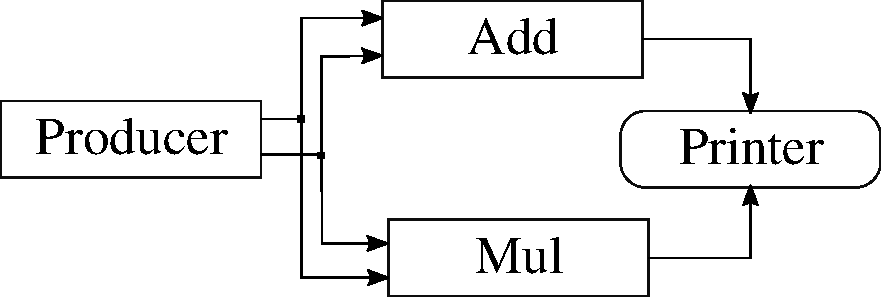
\includegraphics[width=0.6\textwidth]{figures/someopsnet.pdf}
  \caption{Schematics of the SomeOps network. Figure from \cite{asheim2016vhdl}.}
  \label{fig:someops}
\end{figure}

\begin{widefigure}
  \begin{subfigure}[t]{0.49\textwidth}
  \begin{pythoncode}
from sme import *
t = Types()

class Producer(Function):
  def setup(self, ins, outs):
    self.map_outs(outs, "outp")
    self.v1 = 0  # type: t.u7
    self.v2 = 0  # type: t.u7

  def run(self):
    self.outp["val1"] = self.v1
    self.outp["val2"] = self.v2
    self.v1 += 1
    self.v2 += 1
    if self.v1 > 100:
      self.v1 = 0
      self.v2 = 0

class Add(Function):
  def setup(self, ins, outs):
    self.map_ins(ins, "valbus")
    self.map_outs(outs, "addbus")

  def run(self):
    self.addbus["res"] = self.valbus["val1"] +
             self.valbus["val2"]

class Mul(Function): # Snipped (similar to Add)

class Printer(External):
  def setup(self, ins, outs):
    self.map_ins(ins, "addbus", "mulbus")

  def run(self):
    print(self.addbus["res"],
          self.mulbus["res"])

class SomeOps(Network):
  def wire(self):
    valbus = Bus("ValueBus", [t.u7("val1"),
                              t.u7("val2")])
    valbus["val1"] = 0
    valbus["val2"] = 0
    addbus = Bus("AddBus", [t.u8("res")])
    addbus["res"] = 0
    mulbus = Bus("MulBus", [t.u14("res")])
    mulbus["res"] = 0
    prod = Producer("Producer", [], [valbus])
    add = Add("Add", [valbus], [addbus])
    mul = Mul("Mul", [valbus], [mulbus])
    printer = Printer("Printer",
                      [addbus, mulbus], [])
    self.tell(printer) # 6x self.tell snipped
# Main function snipped
\end{pythoncode}
\caption{Original Python SME code.}
\label{fig:someopspy}
\end{subfigure}
\begin{subfigure}[t]{0.49\textwidth}
  \begin{smeilcode}
sync proc Add (in valbus, out addbus)
{
    addbus.res = valbus.val1 + valbus.val2;
}

sync proc Mul (in valbus, out mulbus)
{
    mulbus.res = valbus.val1 * valbus.val2;
}

sync proc Printer (in addbus, in mulbus)
{
    // Manually added
    trace("Add result: {} Mul result: {}",
        addbus.res, mulbus.res);
}

sync proc Producer (out outp)
    var v2: u7 = 0;
    var v1: u7 = 0;
{
    outp.val1 = v1;
    outp.val2 = v2;
    v1 = v1 + 1;
    v2 = v2 + 1;
    if (v1 > 100) {
        v1 = 0;
        v2 = 0;
    }
}

network SomeOps ()
{
    exposed bus AddBus {res: u8;};
    exposed bus MulBus {res: u14;};
    exposed bus ValueBus {val1: u7;
                          val2: u7;};
    instance Add of Add(ValueBus, AddBus);
    instance Mul of Mul(ValueBus, MulBus);
    instance Printer of Printer(AddBus, MulBus);
    instance Producer of Producer(ValueBus);
}

\end{smeilcode}
\caption{Generated SMEIL code.}
\label{fig:someopssme}
\end{subfigure}
\caption{Example of PySME code automatically translated to SMEIL.}
\end{widefigure}


\section{7-Segment Display}
\label{sec:7seg}
\begin{figure}%[tb]
\begin{minipage}{\linewidth}
  \centering
  \resizebox{.6\linewidth}{!}{
    \begin{tikzpicture}[font=\small,
      rep style/.style={rectangle,draw=black,text width=1.5cm,minimum
        size=1.5cm,align=center},
      proc style/.style={ellipse,draw=black,align=center,text
        width=1.5cm,minimum size=1.5cm,align=center},
      file style/.style={ellipse,draw=none,align=center,text
        width=1.5cm,minimum size=0.5cm,align=center},
      part/.pic={
        \node[] (m1) {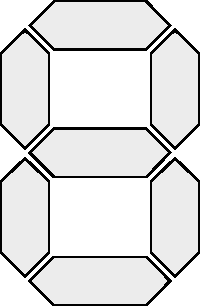
\includegraphics[width=.10\textwidth]{figures/7seg.pdf}};
        \node[left=0cm of m1] (m2) {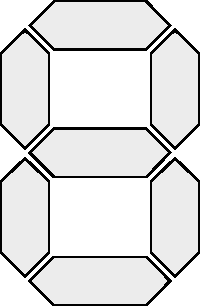
\includegraphics[width=.10\textwidth]{figures/7seg.pdf}};}
      ]

      \pic[local bounding box=hrs] {part};
      \node[below=2mm of hrs] (h2) {Hours};
      \pic[local bounding box=mins, right=30mm of hrs] {part};
      \node[below=2mm of mins] (m2) {Minutes};
      \pic[local bounding box=secs, right=30mm of mins] {part};
      \node[below=2mm of secs] (s2) {Seconds};

      \node[proc style, above=0.3cm of hrs] (dechrs) {Decoder};
      \node[proc style, above=0.3cm of mins] (decmins) {Decoder};
      \node[proc style, above=0.3cm of secs] (decsecs) {Decoder};

      \node[proc style, above=1cm of dechrs] (enchrs) {Encoder};
      \node[proc style, above=1cm of decmins] (encmins) {Encoder};
      \node[proc style, above=1cm of decsecs] (encsecs) {Encoder};
      
      \node[proc style, above=1cm of enchrs] (splithrs) {Calculate\\Hours};
      \node[proc style, above=1cm of encmins] (splitmins) {Calculate\\Minutes};
      \node[proc style, above=1cm of encsecs] (splitsecs) {Calculate\\Seconds};

      \draw[-{Latex[scale=1.6]}] (splithrs) edge (enchrs);
      \draw[-{Latex[scale=1.6]}] (splitmins) edge (encmins);
      \draw[-{Latex[scale=1.6]}] (splitsecs) edge (encsecs);

      \node[above=1cm of splitmins] (split) {};
      
      \node[proc style, above=2.5cm of split] (gen) {Timer};
      \draw[-] (gen) edge node [below left=0cm and 0cm of
      gen] {Seconds today} (split);

      \draw[-{Latex[scale=1.6]}] (split) edge (splithrs);
      \draw[-{Latex[scale=1.6]}] (split) edge (splitmins);
      \draw[-{Latex[scale=1.6]}] (split) edge (splitsecs);

      \draw[-{Latex[scale=1.6]}] (enchrs) edge (dechrs);
      \draw[-{Latex[scale=1.6]}] (encmins) edge (decmins);
      \draw[-{Latex[scale=1.6]}] (encsecs) edge (decsecs);

      \begin{scope}[on background layer]
        \node[draw=gray,inner sep=8pt,rounded corners=10pt,anchor=north
        west,fit=(enchrs)(encmins)(encsecs)(splithrs)(splitmins)(splitsecs)(gen),
        label={above}:Controller]
        (showhrs) {};
        \node[draw=gray,inner sep=8pt,rounded
        corners=10pt,anchor=north west,fit=(hrs)(dechrs)] (showhrs) {};
        \node[draw=gray,inner sep=8pt,rounded corners=10pt,anchor=north
        west,fit=(mins)(decmins)] (showmins) {}; \node[draw=gray,inner
        sep=8pt,rounded corners=10pt,anchor=north west,fit=(secs)(decsecs)]
        (showhrs) {};
      \end{scope}
    \end{tikzpicture}}
    \caption{Model digital clock using a 7-segment display. A timer keeps track
      of the number of seconds elapsed since midnight and several processes
      calculates and lights.
      \protect\footnote{7-segment digit rendering based on ``7
        segment display labeled''
        (\url{https://commons.wikimedia.org/wiki/File:7_segment_display_labeled.svg})
        by h2g2bob. CC BY-SA-3.0.}}
     %\protect\footnotemark}}
\label{fig:7seg}
\end{minipage}
  \end{figure}
    % \footnotetext{7-segment digit rendering based on ``7 segment display labeled''
    % (\url{https://commons.wikimedia.org/wiki/File:7_segment_display_labeled.svg})
    % by h2g2bob. CC BY-SA-3.0.}

  The example implements a model of an old-fashioned digital clock displaying
  the current time using 6 7-segment digits. The layout is depicted in
  \Cref{fig:7seg}. The timer process continuously increments a numeric value,
  representing the number of seconds passed since the beginning of the day,
  which is stored in a process-local variable. For every cycle, the current
  number of seconds is emitted. This number is then broadcasted through a shared
  bus to a number of calculating processes which uses simple integer arithmetic
  to calculate the number of hours, minutes and seconds respectively. To better
  reflect an actual hardware implementation, {\tt encode}r and {\tt decode}r
  processes are inserted on the wire leading to the digit. They, respectively,
  encodes to and decodes from the bit-pattern (represented as hexadecimal
  numbers in the {\tt encode} and {\tt decode} processes) used to light up parts
  of the 7-segment display.

  For representing the current time during simulation, the decoder processes are
  connected to a process which prints the current time in a readable format. The
  code for the process, with elisions, is shown in \Cref{fig:7segcode}.

  A real-world implementation of this design is simple to imagine: The timer
  process is replaced by an actual time-keeping device and the output of the
  encoder processes is connected directly to the 7-segment digits they
  drive. This network is implemented purely in SMEIL without depending on
  external processes for stimuli.

  Since this example contains its own data generation source it is run using the
  command-line interface of \libsme{}. The result of executing this network is
  shown below.
\begin{verbatim}
$ smec -i 7seg.sme -s 50  
00:00:00
00:00:00
00:00:00
00:00:00
00:00:01
00:00:02
00:00:03
[..]
\end{verbatim}
  Note that the depth of the network is visible in that it takes a few cycles
  before the first time has propagated to the printer.
  
  \begin{widefigure}
    \centerfloat
\begin{lstlisting}[multicols=2, language=smeil]
proc timer ()
  bus elapsed {
    secs: uint;
  };
  const secs_per_day: uint = 86400;
  var cur: u17;
{
  cur = (cur + 1) % secs_per_day;
  elapsed.secs = cur;
}

proc hrs (in time)
  bus vals {
    d1: uint;
    d2: uint;
  };
  const secs_per_hr: uint = 3600;
  var cur: uint;
{
  cur = time.secs/secs_per_hr;
  vals.d1 = cur/10;
  vals.d2 = cur%10;
}

// [..]

proc encode (in inval)
  bus vals {
    d1: uint;
    d2: uint;
  };
  const digits: [10]uint =
    [0x7E, 0x30, 0x6D,
     0x79, 0x33, 0x5B,
     0x5F, 0x70, 0x7F,
     0x7B];
{
  vals.d1 = digits[inval.d1];
  vals.d2 = digits[inval.d2];
}

proc decode (in inval)
  bus vals {
    d1: uint;
    d2: uint;
  };
{
  switch inval.d1 {
    case 0 {vals.d1 = 0; }
    case 0x7E { vals.d1 = 0;}
    // [..]
    case 0x7B { vals.d1 = 9;}
    default { assert(false); }
  }
  //[..]
}

proc disp (in val1, in val2, in val3) {
  trace("{}{}:{}{}:{}{}",
    val1.d1, val1.d2,
    val2.d1, val2.d2,
    val3.d1, val3.d2);
}

network clock() {
  instance t  of timer();
  instance h  of hrs(t.elapsed);
  instance ench of encode(h.vals);
  instance dech of decode(ench.vals);
  // [..]
  instance _ of disp(dech.vals,
                     decm.vals,
                     decs.vals);
}
\end{lstlisting}
    \caption{Code of the 7-segment digital clock network.}
  \label{fig:7segcode}
\end{widefigure}  


\section{ColorBin}
\label{sec:colorbin}
\begin{figure}%[tb]
  \centering
  \resizebox{.7\linewidth}{!}{
    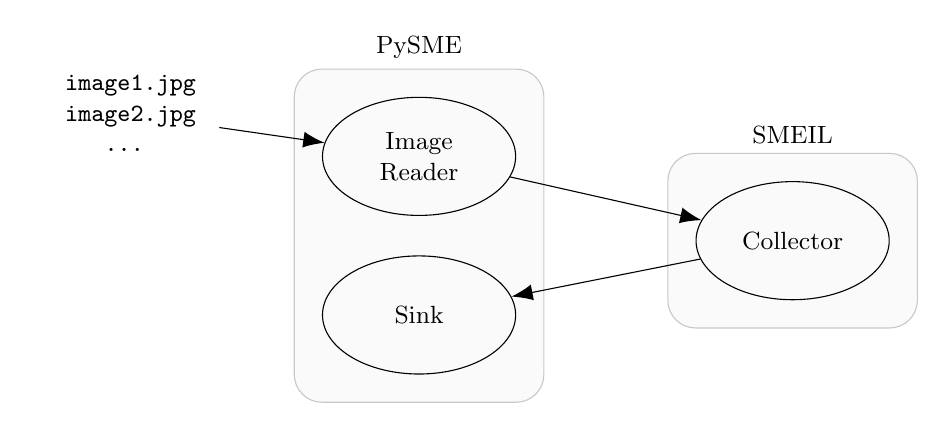
\begin{tikzpicture}[font=\small,
      rep style/.style={rectangle,draw=black,text width=1.5cm,minimum
        size=1.5cm,align=center},
      proc style/.style={ellipse,draw=black,align=center,text
        width=1.5cm,minimum size=1.5cm,align=center},
      file style/.style={ellipse,draw=none,align=center,text
        width=1.5cm,minimum size=0.5cm,align=center}
      ]
      \node[file style] (ims) {\ttfamily image1.jpg \\ \ttfamily image2.jpg \\ \ttfamily ...};
      
      \node[proc style, below right=-0.6cm and 2cm of ims] (gen) {Image \\ Reader};
      \node[proc style, below right=0cm and 3cm of gen] (collector) {Collector};
      \node[proc style, below=0.5cm of gen] (sink) {Sink};

      \draw[-{Latex[scale=1.6]}] (ims) edge (gen);
      \draw[-{Latex[scale=1.6]}] (gen) edge (collector);
      \draw[-{Latex[scale=1.6]}] (collector) edge (sink);
      
      \begin{scope}[on background layer]
        \node[draw=scopeborder,fill=scopebg,inner sep=10pt,rounded corners=10pt,anchor=north west,fit=(collector),label={above}:SMEIL] (SMEIL) {};
        \node[draw=scopeborder,fill=scopebg,inner sep=10pt,rounded corners=10pt,anchor=north west,fit=(gen)(sink),label={above}:PySME] (pysme) {};
      \end{scope}
    \end{tikzpicture}
  }
  \caption{The process network of ColorBin.}
  \label{net:colorbin}
\end{figure}


This network, named ColorBin (ported from the C\# version in
\cite{skovhede2017c++}), serially process the pixels in one or more images and
categorize their intensity as low (closer to black), medium and high (closer to
white). The generator reads images from the disk and separates each of their
pixels into RGB components. The input bus also contains a boolean signal which
is true along with the last pixel of each image, acting as a token to signify
the end of an image. That way, the collector process (described next) can tell
the images apart and reset its counters when a new image begins. The collector
process examines each pixel, incrementing one of three intensity counter
variables as appropriate. When it receives the last-pixel token, it sends the
stored values of the intensity counters to the sink process which then collects
the pixel intensity counts for each image.

The SMEIL source code for the collector process is shown in
\Cref{fig:collector}. The VHDL code generated for the process is shown in
\Cref{fig:vhdlc}. The mapping of names and structure from SMEIL to VHDL is
clearly seen, as is the immense verbosity of VHDL. When we generate expressions,
we set parentheses in a very pessimistic manner. To ensure that the precedence
of operators in SMEIL is preserved in VHDL, we set parentheses around every
binary operation. Unfortunately, this adds some clutter to the generated code in
the form of unnecessary parentheses. This matter is subject to future
improvements, for example, by implementing the ``unparsing'' method described in
\cite{ramsey1998unparsing} which, based on knowledge about operator precedence
in the target language, reverse-transforms an AST using as few parentheses as
possible.

This SMEIL network gets its data through co-simulation with a PySME
network. Therefore, it is executed by running the Python-end of the network. As
input to this network we provide three separate images. As output, it simply
prints the pixel intensity statistics. In \Cref{sec:perf}, we provide a
benchmark comparing the time required for running this network on the three
images both by simulating the original SMEIL code and the generated VHDL code.

\begin{widefigure}

\begin{lstlisting}[language=smeil,multicols=2]
proc collector (in image_input)
  exposed bus bin_count_out {
    valid: bool;
    low: u32;
    med: u32;
    high: u32;
  };
// [..]
{
  if (image_input.valid) {
    color = ((image_input.R * 299) +
      (image_input.G * 587) +
      (image_input.B * 114)) / 1000;

    if (color > thresh_high) {
      counthigh = counthigh + 1;
    } elif (color > thresh_med) {
      countmed = countmed + 1;
    } else {
      countlow = countlow + 1;
    }
  }

  bin_count_out.low = countlow;
  bin_count_out.med = countmed;
  bin_count_out.high = counthigh;
  bin_count_out.valid =
    image_input.valid &&
    image_input.last_pixel;
}
\end{lstlisting}
  \caption{SMEIL source code for the collector process of the ColorBin network.}
  \label{fig:collector}
\end{widefigure}

\begin{widefigure}[hb!]
\begin{lstlisting}[language=vhdl]
entity collector is
  port (
    signal bin_count_out_valid: out boolean := false;
      -- [..]
  signal bin_count_out_high: out unsigned (31 downto 0) := to_unsigned(0, 32);
  signal image_input_valid: in boolean;
  -- [..]
  signal image_input_B: in unsigned (7 downto 0);
  signal clk: in std_logic;
  signal rst: in std_logic);
end entity collector;

architecture rtl of collector is
begin
  process (clk, rst) is
    constant thresh_high: integer := 200;
    -- [..]
    variable countlow: unsigned (31 downto 0) := to_unsigned(0, 32);
  begin
    if rst = '1' then
      bin_count_out_valid <= false;
      bin_count_out_low <= to_unsigned(0, 32);
      -- [..]
      countlow := to_unsigned(0, 32);
    elsif rising_edge(clk) then
      if image_input_valid then
        color := resize(((((((image_input_R *
                              to_unsigned(299, 10))) +
                            ((image_input_G * to_unsigned(587, 10)))) +
                           ((image_input_B * to_unsigned(114, 10))))) /
                         to_unsigned(1000, 10)),  color'length);
        if (color > thresh_high) then
          counthigh := resize((counthigh + to_unsigned(1, 32)),
                              counthigh'length);
        -- [...]
        end if;
      end if;
      bin_count_out_low <= resize(countlow, bin_count_out_low'length);
      -- [..]
\end{lstlisting}
  \caption{The VHDL code generated from the SMEIL code shown in
    \Cref{fig:collector}.}
  \label{fig:vhdlc}
\end{widefigure}

  
\section{High-frequency trading chip}
\begin{figure}%[tb]
  \centering
  \resizebox{.9\linewidth}{!}{
    \begin{tikzpicture}[font=\small,
      rep style/.style={rectangle,draw=black,text width=1.5cm,minimum
        size=1.5cm,align=center},
      proc style/.style={ellipse,draw=black,align=center,text
        width=1.5cm,minimum size=1.5cm,align=center},
      file style/.style={ellipse,draw=none,align=center,text
        width=1.5cm,minimum size=0.5cm,align=center},
      plot/.pic={
        \node[] (m1) {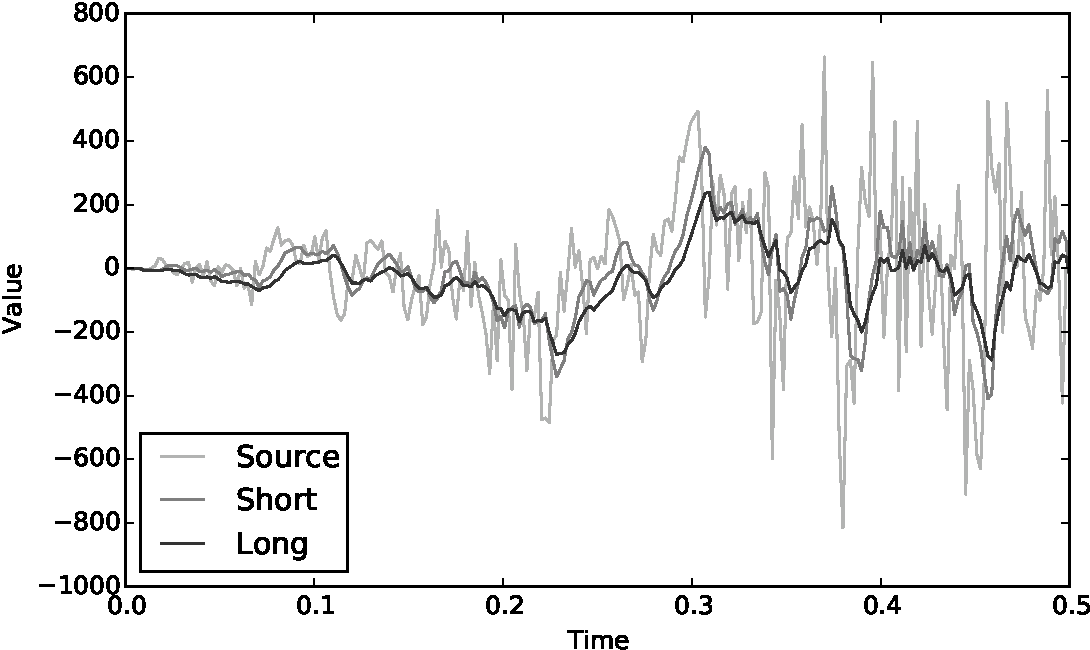
\includegraphics[width=.25\textwidth]{figures/ewma-plot.pdf}};
      }
      ]

      
      \node[proc style] (gen) {Data \\ Generator};
      \node[proc style, right=2cm of gen] (long) {Short Decay};
      \node[proc style, below=0.5cm of long] (short) {Long Decay};
      \node[proc style, below right=0cm and 1.5cm of long] (merge) {Merger};

      \node[proc style, below=0.5cm of gen] (sink) {Plotter};

      \pic[local bounding box=plot, above left=0cm and 2cm of sink] {plot};
      
      \draw[-{Latex[scale=1.6]}] (gen) edge (long);
      \draw[-{Latex[scale=1.6]}] (gen) edge (short);
      \draw[-{Latex[scale=1.6]}] (long) edge (merge);
      \draw[-{Latex[scale=1.6]}] (short) edge (merge);
      \draw[-{Latex[scale=1.6]}] (sink) edge (plot);

      % \draw[-{Latex[scale=1.6]}] (gen) edge (collector);

      \draw[-{Latex[scale=1.6]}] (merge) edge [bend left=50] (sink);
      
      \begin{scope}[on background layer]
        \node[draw=scopeborder,fill=scopebg,inner sep=10pt,rounded corners=10pt,anchor=north west,fit=(long)(short)(merge),label={above}:SMEIL] (SMEIL) {};
        \node[draw=scopeborder,fill=scopebg,inner sep=10pt,rounded corners=10pt,anchor=north west,fit=(gen)(sink),label={above}:PySME] (pysme) {};
      \end{scope}
    \end{tikzpicture}
  }
  \caption{The network of simpletrader.}
  \label{fig:simpletrade}
\end{figure}
We revisit an example from~\cite{asheim2016vhdl}. In high-frequency trading, a
split-second decision needs to be made whether to buy, or sell, a
stock. Reducing latency is paramount as you need to make transactions as fast as
possible. This problem is, therefore, an interesting target for custom hardware
as the intractable latencies induced by general-purpose hardware and
software-implemented decision-making logic are avoided. The real-time value of a
stock is passed through two calculator processes. Both calculate the exponential
moving average of a stock, one using long decay and the other using short
decay. The trading decision is based on detecting when the two averages
cross.~\cite{kablan2012use}

The network is shown in \Cref{fig:simpletrade} and the SMEIL source in
\Cref{fig:tradesrc}. The results of the two calculator processes described above
is passed through the merge process which combines the long and short averages
into a single bus. The core of the trader is written in SMEIL, while the
processes providing input stimuli and data collections is written in Python as a
PySME model. The input data is generated using a Brownian
bridge~\cite{glasserman2003monte} which is a stochastic process commonly used as
a model for simulating realistic stock price developments. The results are
collected and visualized in a graph for easy verification.

In an actual trading chip, the data generator is replaced with actual stock
prices arriving through a network interface and the plot is replaced by market
transactions. Both the testing and verification processes leverage existing
Python libraries. The Brownian bridge generator is implemented using NumPy while
the plot is made using {\ttfamily matplotlib}. Implementing these test processes
in VHDL would be a massive undertaking, with Python, it is quite simple.

We execute this example by calling the Python script containing the PySME part
of the implementation which will then execute together with the part of the
network written in SMEIL via the co-simulation interface. The Python part of the
network shows a graph visualizing the moving averages.

The test bench generated along with the VHDL code runs without errors and prints
the message
\begin{verbatim}
ewma_tb.vhdl:166:13:@1275001275ns:(report note): completed
  successfully after 255 clockcycles
\end{verbatim}
on completion.

\begin{widefigure}
  \begin{smeilcode2}
sync proc calc (in data, const decay)
  bus result {
    val: int;
    valid: bool;
  };
  var prev: int;

{
  if (data.valid) {
    result.valid = true;
    prev = (data.val >> decay) +
      (prev >> decay) *
      ((1 << decay) - 1);
    result.val = prev;
  } elif (!data.valid) {
    result.val = prev;
  } else {
    result.valid = false;
  }
}

sync proc merge (in long,
                 in short, out res) {
  if (long.valid && short.valid) {
    res.valid = true;
    res.long = long.val;
    res.short = short.val;
  } else {
    res.valid = false;
  }
}

network ewma () {
  const decay1: int = 2;
  const decay2: int = 3;

  exposed bus stream {
    val: int;
    valid: bool;
  };

  exposed bus output {
    short: int;
    long: int;
    valid: bool;
  };

  instance short of calc 
      (data: stream, decay: decays1);
  instance long of calc
      (data: stream, decay: decays2);
  instance _ of merge
      (long: long.result,
       short: short.result,
       res: output);
}
\end{smeilcode2}
\caption{SMEIL source code for the trader core.}
\label{fig:tradesrc}

\end{widefigure}


\section{MD5 bruteforcer}
\label{sec:md5}
\begin{figure}%[tb]
  \centering
  \resizebox{.6\linewidth}{!}{
    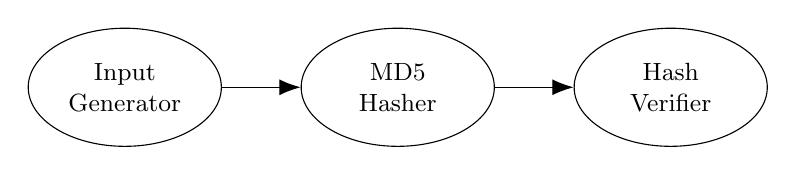
\begin{tikzpicture}[font=\small,
      rep style/.style={rectangle,draw=black,text width=1.5cm,minimum
        size=1.5cm,align=center},
      proc style/.style={ellipse,draw=black,align=center,text
        width=1.5cm,minimum size=1.5cm,align=center},
      file style/.style={ellipse,draw=none,align=center,text
        width=1.5cm,minimum size=0.5cm,align=center}
      ]

      \node[proc style] (gen) {Input\\Generator};
      \node[proc style, right=1cm of gen] (calc) {MD5 Hasher};
      \node[proc style, right=1cm of calc] (verify) {Hash\\Verifier};

      \draw[-{Latex[scale=1.6]}] (gen) edge  (calc);
      \draw[-{Latex[scale=1.6]}] (calc) edge  (verify);

    \end{tikzpicture}}
  \caption{Structure of the MD5 bruteforcer network.}
  \label{fig:md5net}
\end{figure}

This example is a simplification of a bruteforcer of MD5-hashes developed to
showcase the performance of FPGAs in comparison with CPUs and GPGPUs for a
trivially parallelizable problem: Bruteforcing an MD5
hash~\cite{johnsen2018md5}. The layout of the network is shown in
\Cref{fig:md5net}. The generator iteratively emits all combinations of 8 ASCII
printable characters as a string. This string is then passed to the hasher,
calculating the MD5 sum of the string. In the verifier, the calculated hash is
compared to a pre-calculated hash of the input string that we wish to find. The
predictiveness of the input generator means that we can ensure that the search
terminates quickly by choosing a target string close to the starting
string. Hence, short runs can be chosen for testing and long runs for
benchmarking.

A complete implementation of this example exists for several targets: CPUs
parallelized with OpenMP, OpenCL for GPGPUs, Xilinx HLS and finally C\# SME.
Both the two latter implementations synthesizes and runs on FPGAs. A comparison
of these implementations showed that while GPUs were superior in raw
performance, the performance-per-watt ratio favored FPGAs by more than an order
of magnitude. Furthermore, the SME version is significantly more efficient than
the Vivado HLS implementation, which relies on the concurrency inference
discussed in the introduction.

This example mainly serves to show an SMEIL implementation of an SME model which
has been synthesized to an FPGA. It also showcases an implementation of a
non-trivial algorithm (MD5) in SMEIL. In particular, the MD5 algorithm relies
heavily on bit-shifting of 32-bit unsigned integers. Therefore, it depends on
the correctness of the integer overflow emulation of the \libsme{} simulator in
order to produce the expected result. The shortened source code of the SMEIL
process for calculating an MD5 hash is shown in \Cref{fig:smeilhash}. The
process receives the string that should be hashed through the bus passed as its
{\ttfamily input} parameter. The calculated hash is then sent on the {\ttfamily
  hashes} bus which is read by the verification process.

Since this network contain its own data generation source this network is run
using the command line interface of \libsme. A session is shown below
\begin{verbatim}
$ smec -i md5-simple.sme --no-warnings -s 50 
[..]
verifying hash 3141438837 2285911344 1677794538 2336503479
verifying hash 1449451250 1644770476 3741827633 1220464617
1449451250 1644770476 3741827633 1220464617 found
\end{verbatim}
where the bruteforcer network is configured to run for 50 cycles. The hash to
look for has been pre-programmed in the verifier. Every tested hash is printed
until the correct one is found. We have verified this implementation by testing
it against the C-implementaiton of the same algorithm, ensuring that they
produce identical results. On a side note, support for printing hexadecimal
numbers should defenitely be added in future versions of SMEIL.


%Also note the close
% resemblance of the SMEIL implementation of the algorithm to an eq

\begin{widefigure}

\begin{smeilcode2}
proc md5(in input)
  bus hashes {
    h0: u32;
    h1: u32;
    h2: u32;
    h3: u32;

    w0: u32;
    w1: u32;
  };

  const r: [64]uint = [
    [...]
    6, 10, 15, 21, 6, 10]

  const kk: [64]uint = [
    0xd76aa478, 0xe8c7b756
    [..]
    0xf7537e82, 0xbd3af235
    ];

// Variable declarations omitted

{
  h0 = 0x67452301;
  // [..]

  w[0] = input.w0;
  w[1] = input.w1;
  w[2] = 128;
  w[14] = 64;

  a = h0;
  b = h1;
  c = h2;
  d = h3;

for i = 0 to 63 {
  if (i < 16) {
    f = (b & c) | ((~b) & d);
    g = i;
   // [..]
  } else {
    f = c ^ (b | (~d));
    g = (7 * i) % 16;
  }

  tmp = d;
  d = c;
  c = b;
  x = a + f + kk[i] + w[g];
  c2 = r[i];
  b = b + (((x) << (c2)) |
      ((x) >> (32 - (c2))));
  a = tmp;
}

h0 = h0 + a;
// [..]
h3 = h3 + d;

hashes.h0 = h0;
// [..]
hashes.h3 = h3;

hashes.w0 = w[0];
hashes.w1 = w[1];
}

\end{smeilcode2}
  \caption{SMEIL source code for the MD5 hashing process.}
  \label{fig:smeilhash}

\end{widefigure}

\section{Performance}
\label{sec:perf}
The simulation performance of a hardware design tool is not essential as it does
not have an impact on the resulting implementation. Nevertheless, a slow
simulator can waste valuable developer time by inducing a long
develop-compile-test cycle.

The current implementation of SMEIL is not written with performance in mind and
leaves a lot of performance-related low-hanging fruits unpicked. Indeed, its
naïve interpreter makes repeated traversals of the SMEIL AST and the interface
between PySME and \libsme{} relies on the very general and inefficient
\texttt{libffi} library.
% Lastly, Python itself is not cherished for its
% performance. It is therefore noteworthy that it still exceeds the performance of
% the VHDL simulator GHDL,
Lastly, Python itself is not cherished for its performance. In spite of this,
\libsme{} still exceeds the performance of the VHDL simulator, GHDL, which
generates native code before simulating. The VHDL simulator of Xilinx Vivado,
fails to complete the simulation due to memory exhaustion.

Simulating 352,686 cycles of the ColorBin (\Cref{sec:colorbin}) network on an
Intel Core i7 6700HQ CPU at 2.60GHz, requires 47 seconds using GHDL but only 30
seconds using \libsme. Based on the benchmarks shown in \cite{skovhede2017c++},
\libsme{} achieves only slightly worse performance than C\# SME in this
particular test.


%%% Local Variables:
%%% mode: latex
%%% TeX-master: "../master"
%%% TeX-command-extra-options: "-enable-write18"
%%% End:

\chapter{Discussion}

% In the previous chapters, we have described a new language for representing SME
% networks, SMEIL and how its implementation fits into the greater whole
% \todo{rewrite}. The questions that are left to answer now are, what have we
% achieved by doing so? Is SMEIL suitable for the current SME ecosystem, and
% finally,

We started working on SMEIL with the intention of creating an intermediate
representation for use with existing SME implementations. The resulting language
covers a wider scope and has a larger number of use cases than was originally
intended. In this chapter, we discuss uses for SMEIL and how it relates to
current SME implementations.

% \section{Completeness of SMEIL in relation to SME}
% In this section, we try to provide some insight into whether the SMEIL provides
% a {\itshape complete} representation of the SME model. Thus, a complete SME
% implementation is \begin{inparaenum}]a)] \item able to construct networks from 
% \end{inparaenum}

% A complete SME implementation implements all the key elements of the SME model
% including
% \begin{itemize}
% \item Independent processes
% \item Buses
% \item Synchronous communications
% \item Ability to create compositions of networks.
% \end{itemize}
% as SMEIL features all of these, we believe it to be able to provide 

% As we have shown in several examples. 

% Before SMEIL is able to be used 
% A shortcoming of SMEIL in its current state is that we do not yet support all of
% the features of the C\# SME implementation, however, doing so was not within the
% scope of the thesis in the first place.


\section{Usability of SMEIL}
As a language for representing SME networks SMEIL is complete in the sense that
it implements the elements and semantics required by the SME model. We have also
shown a number of actual implementations of SME networks showing the practical
use of SMEIL. Thus, SMEIL is capable of representing the SME models which are
currently implemented in other languages.

% This is shown here through the numerous examples that we have been able to
% implement.
% An issue which we have not discussed is how well SMEIL scales for
% larger networks since we have only looked at small examples. For this, we argue
% that the scalability of SMEIL is similar to that of C\# SME which has previously
% been used to create large-scale SME implementations. This is because the primary
% structural components of the C\# SME implementations maps to SMEIL in a
% straight-forward manner.


We have previously argued for the potential benefits of using SMEIL in favor of
general-purpose for writing hardware-targeted SME models. However, there are
also several disadvantages related to implementing a new and distinct
language. One particular disadvantage is the abandonment of development
environments, debuggers and other tooling that comes with an established
general-purpose language. For SMEIL to offset these disadvantages, an additional
development effort is required to replace this tooling. On the other hand,
debuggers for conventional programming languages are not well suited for
debugging concurrent models, such as SME. Therefore, introducing a new language,
may create an avenue for creating new tooling which are better suited for their
purpose.

% On the other hand,
% in relation to debuggers it could be argued that languages for constructing
% concurrent models, such as SMEIL, require a different kind of debuggers than
% traditional sequential languages.


% Another aspect which is outside the scope of the thesis is actually implementing
% the generated VHDL code on hardware. However, it is still an important aspect to
% discuss since the primary purpose of writing SME models is to, as previously
% mentioned, eventually create a hardware description....


\subsection{Using SMEIL as an IL}
SMEIL is usable as an intermediate language for SME models written in a wide
range of different general-purpose languages. The static structural definitions
and the static type system of SMEIL forces a normalized representation of SME
networks regardless of which source language the SMEIL code was generated
from. Thus, when generating SMEIL from a dynamically typed source, it is the
responsibility of the generator to ensure that the appropriate types are
assigned. In PySME, for example, this problem was solved by allowing
type-annotations to be written in comments. The result of this, is that a SMEIL
program should not inherit any particular traits of the code that it was
generated from. Therefore, SMEIL will allow combining SME networks that was
originally written in different source languages.

We have already shown an example of how SMEIL can function as an intermediate
language for the PySME SME implementation. However, the PySME library is
restricted in terms of functionality compared to the C\# SME library which has
been used as the base for all of the previously referenced SME models
implemented on hardware. Compared to C\# SME, SMEIL and \libsme{} still lacks a
number of essential features. Achieving feature-parity with ``state-of-the-art''
SME libraries was considered outside the scope of this thesis due to the longer
period of time that these libraries has been under development. However, it
means that more work is required in order to make SMEIL usable as an IL for C\#
SME.

% \section{Relation with other HDLs}
% Discuss how SME and specifically SMEIL relates to other similar ``simple''
% hardware description languages. \todo{Should this be here?}

% \section{Related co-simulation approaches}
% \todo{Should this be here}

% \section{Comparison with ``state-of-the-art'' SME}
% Write about: Internal buses: We have language support based on inference from
% usage, but not implemented. Arrays as buses

\section{Co-Simulation and observation based typing}
One of the strongest features of SMEIL is the co-simulation interface which
allows it to seamlessly interact with SME networks written in other
languages. It is the cornerstone of enabling SMEIL to be used both as an
intermediate language and as a primary implementation language for SME models in
a capable manner. For the intermediate-language use case it helps simplifying
the implementation of SME libraries using it. For example by offloading the
generation of trace-files. For use as a primary implementation language, it
allows direct testing of designs without having to execute generated
code. Furthermore, the co-simulation interface is central in enabling a tightly
integrated implementation of the system for observation-based typing.

Co-simulation is a frequently used technique for verifying hardware designs (see
e.g. CoCoTB referenced in \Cref{sec:retwork}), however, the presented SME-based
solution is unique in that the same model is used on both sides of the
simulation. As one particular advantage, the compositionality of SME means that
a process may be moved seamlessly between both sides of the Co-Simulation.  We
have only shown an implementation of the API for Python here but we believe that
extending other SME implementations with support for the \libsme co-simulation
API will be possible. This is the case since the API is kept ``as close to C''
as possible. Hence, any language featuring a capable C interface should be able
to use it.

% Due to the dynamic nature of Python it lends itself well for performing
% such...

Our approach for determining types based on observed input is, to the best of
our knowledge, also not implemented in any existing HDLs. We are aware that
there may be good reasons for this, due to the, as previously mentioned,
inadequate safety provided by this approach. However, based on our limited
testing, the productivity advantage of not having to place precise type bounds
on all internal variables does seem to be real. Furthermore, in some cases, such
as quickly prototyping a design on a FPGA, safety may not be the primary desired
features. Thus, if combined with static analysis to prove that the
observationally derived type bounds really are safe, it may turn out to be a
powerful approach.

\section{Target Language Support}
We have currently only implemented a code generation backend for VHDL. We
focused on supporting VHDL since the primary intended target for SME models are
hardware designs. For this thesis, we chose not to implement support for
additional code generation backends and instead making the core infrastructure
related to SMEIL as complete as possible. However, having support for generating
additional languages is desirable in several circumstances. Having, for example,
C++ support will, as shown in \cite{skovhede2017c++}, allow for faster
simulation of SME networks and allow SME networks to be used as independent
libraries with other languages.

Supporting other HDLs, such as Verilog, is also desirable since it would allow
SME models to interface with hardware designs implemented in HDLs other than
VHDL. Adding such support to SMEIL is quite feasible since most other ``new''
HDLs (we do a small survey in \Cref{sec:retwork}) support code generation for at
least VHDL and Verilog. This shows that hardware designs which are implemented
in VHDL can also be represented using Verilog.

The current \libsme{} implementation is written with support for multiple target
languages in mind. This is done, by confining all VHDL-related details to the
VHDL code generation backend. All other phases of the compiler are kept as
general as possible. Thus, we do not foresee any problems related to adding
additional code-generation backends for SMEIL.

We have not assessed the practicality of transforming SMEIL to languages
following other paradigms, such as functional languages or alternative hardware
description languages. So far, however, there has not been a need for SME models
to be able to target such languages.


% However, compiling SMEIL to other languages, such as C++ ) is also desirable. Furthermore, \libsme is written with
% support for multiple target languages in mind, and the infrastructure to add
% another target language is in place, but unfortunately time constraints did not
% allow us to do it. Specifically in relation to other HDLs such as Verilog. Most
% new high-level HDLs is able to generate at lest VHDL and Verilog. SME is
% currently only translatable to VHDL, however, adding support for Verilog is
% entirely possible. To support this claim, we point
% to \begin{inparaenum}[a)]\item The large number of tools (e.g. \todo{cite})
%   )already supporting both languages and \item numerous \end{inparaenum}
% \todo{cite} \todo{Why do we think its simple to add another language?}

%%% Local Variables:
%%% mode: latex
%%% TeX-command-extra-options: "-enable-write18"
%%% TeX-master: "../master"
%%% End:

\chapter{Conclusions}

% \section{Related work}

% \section{Future Work}

% A key assumption of this work is that we assume that input values explore the
% value ranges of SME buses. In many cases, this assumption may be impractical as
% the quality of test-cases has an enormous impact on the correctness and
% usefulness of the resulting implementation. To address this, methods for
% inferring the value ranges of SME buses using purely static means may also be
% useful.

% Allow \gls{vhdl} code to be embedded within \gls{smeil} and simulate by linking
% the simulation to a \gls{vhdl} simulator using \gls{vhpi}. This is similar to
% work done by cocotb and clash master

\section{Related Work}
\label{sec:retwork}
% Work related to SMEIL centers around two different areas; high level languages
% for implementing hardware designs mention.

% Xilinx HLS attempts to infer concurrency from sequential C programs guided by
% annotations and use that to generate hardware descriptions. A drawback of this
% approach is that the quality of the resulting hardware implementation depends
% greatly on the quality of the added annotations. SME takes a different approach
% in being explicit about the concurrency of the resulting hardware design.

In addition to the HLS approaches mentioned in the introduction, several
alternative hardware design modeling tools have been proposed both in the
industry and in academia. Furthermore, a number of approaches to replace test
benches written in traditional HDLs has been proposed.

MyHDL~\cite{myhdl} is a Python-based HDL, essentially a DSL embedded in
Python. It is intentionally implemented as a high-level version of traditional
HDLs while enabling Python to be used for test benches. Since it inherits its
worldview from traditional HDLs, it has a different goal than SME which provides
an abstraction through the SME model.

Cx~\cite{cxlang} is a dedicated DSL for writing hardware designs. The Cx
language has several similarities with SMEIL, for example, the type system. Like
SME, it allows the programmer to explicitly control concurrency by building
networks of processes. However, despite claims on its website, Cx is a
proprietary language requiring a license for long-term use, giving it a high
barrier-of-entry.

C\textlambda{}aSH~\cite{wester2015transformation} and Lava\cite{bjesse1998lava}
are two Haskell based approaches with different philosophies: Lava is a Haskell
design pattern (with several implementations e.g., \cite{gill2009introducing})
for specifying composable circuits at the gate-level. The extremely low-level
approach means that it is targeted towards replacing and formalizing certain
low-level uses of HDLs rather than as a general high-level hardware modeling
tool. C\textlambda{}aSH, on the other hand, transforms a subset of high-level
Haskell code to HDLs. This requires concurrency inference, but this is simpler
to do for a purely functional language, such as Haskell, compared to an impure
imperative language, such as C.

A more recent approach~\cite{aronsson2017hardware} also uses Haskell, but only
as a host for an Embedded DSL. This EDSL translates to both VHDL and C, enabling
the programmer to trivially change which parts of her program that runs on the
CPU or the FPGA. The library automates setting up AXI interconnects between the
CPU-part and the FPGA-part of the code. The advantage of this approach is that
it enables simple hardware-software co-design. The primary disadvantage of this
approach is that the CPU code must also be written in the DSL. For many
applications, this can be overly restrictive since reuse of existing code and
common libraries is not possible.

CAPF~\cite{serot2011implementing}, Pyrope~\cite{pyrope} and
Chisel~\cite{bachrach2012chisel} are HDLs which provide data-flow based design
models. CAPF and Pyrope are independent languages while Chisel is an EDSL in
Scala. The data layouts that are good fits for these languages are also
expressible using SME, albeit less elegantly. However, problems which are best
represented as a sequential algorithm can be a poor fit for the data-flow
paradigm.

The Coroutine Co-Simulation Test Bench (CoCoTB)~\cite{cocotb} also implements a
notion co-simulation between Hardware Descriptions and Python (A General-Purpose
language). Using the Verilog Procedural Interface (VPI) which (despite the name)
is implemented by both VHDL and Verilog simulators. This library presents a
significant advantage over writing test benches exclusively in HDLs, however,
the relative complexity of the VPI interface leaks into the CoCoTB interface,
requiring a non-trivial amount of boilerplate code. Furthermore, it does not
directly address the productivity issues associated with traditional HDLs and
does not offer the unified simulation model used in SME.


\section{Future Work}
Other SME implementations, C\# SME in particular (see
e.g.~\cite{skovhede2018statemachine}) have evolved in parallel with the
development of SMEIL. Therefore, these are more comprehensive and support a
wider range of features. Since SMEIL is, as previously mentioned, intended to
serve as the only target language for SME, SMEIL should be brought on-par with
other existing SME implementations. In the present work, a substantial amount of
compiler-infrastructure groundwork has been laid, making these improvements a
natural continuation of future SMEIL developments.

As the primary target for SMEIL is hardware, VHDL is the only code generation
backend currently implemented. However, code-generation backends for additional
languages should be added. For example, generating C++ code can make it possible
to use SME programs with other software as a library and provide significantly
faster simulation than the current interpretation-based approaches are able to
offer~\cite{skovhede2017c++}.

All SME implementations currently target a single clock domain. Future efforts
should be made towards supporting multiple clocks, running at different speeds.

In some cases, SMEIL may offer an insufficient amount of control over the
generated VHDL code or the generated code may simply be inefficient compared to
hand-optimized VHDL code. For this, we should allow inlining VHDL inside SMEIL
by adding language constructs to specify how SME buses should be connected to
VHDL signals. The simulation of such mixed code can be performed by running VHDL
parts in a VHDL simulator.

Hardware-software co-design is an area that is actively researched. The idea is
that specialized hardware is designed in parallel with the corresponding
software such that each part of the design can be implemented on either hardware
or software depending on what is best suited. Such heterogeneous designs require
code for setting up the communication between the hardware and software
parts. We should therefore extend our co-simulation approach to also allow SME
networks to be distributed across several devices.

% SME is
% well suited for this and we should, therefore, try to develop a mechanism
% allowing communication between SME networks running on different devices where
% the actual generation of the communication interfaces is handled transparently.

The presented approach, for automatically typing SMEIL networks based on
observed input, makes the assumption that the complete possible space of input
values is explored by the testing stimuli. The downside of this approach is that
this assumption may be hard to fulfill. To address this, the current approach
could be augmented by integer range analysis for proving the observed ranges.

To improve the user-friendliness and capabilities of SMEIL, there is a wide
range of language features that we would like to add. A non-exhaustive list
follows:
\begin{itemize}
\item In practice, not being able to add declarations, such as constants,
  enumerations. and functions, at the top-level of a SMEIL program proved too
  restrictive. This should be added.
\item A syntax for direct bit manipulations. Currently, bit manipulation can
  only be performed through bitwise operators in a similar manner to C. It would
  be convenient to have an array-like syntax for achieving the same thing. The
  syntax could, for example, be similar to Python's array slicing feature.
\end{itemize}

\section{Conclusion}
We have presented SMEIL, a DSL for implementing SME networks and demonstrated
its practical use through several examples. Although we have focused on using it
as a primary implementation language for SME networks, it is also usable as an
intermediate language for other SME implementations. We have shown this by
providing a SMEIL code-generation backend for a Python to VHDL compiler.

SMEIL is based on the structural components of the SME model and provides a
high-level C-like syntax with constructs commonly found in general-purpose
imperative languages. This is needed in order to ensure that SME networks
implemented in general-purpose languages can be translated without requiring
sophisticated transformations.

The type system presented supports bit precise types which is an important
feature for a hardware-targeted language. However, the requirement to
specify a fixed bit-width for all types is sometimes impractical. Instead,
arbitrary-length types may be specified which are then constrained based on
values observed during simulation.

Simulation of SMEIL is performed in a manner which provides a cycle-accurate
representation of the resulting hardware. During the simulation, a trace of
channel communications is recorded. SMEIL compiles to readable VHDL code which
can be used for a subsequent hardware implementation. Additionally, a test bench
is generated which can be used to verify the correctness of the generated
code. The test bench uses the trace recorded during simulation to allow
continuing verification of the generated code even following manual refinement.

For testing SMEIL networks directly, an interface is provided for performing
co-simulation with SME networks written in general-purpose languages. This
approach proved highly successful in practice.

The presented language and its implementation do not yet provide the full
feature-set of other, more mature, SME implementations. In spite of this, we are
optimistic about its future prospects, both as an intermediate language and as
an independent DSL for writing SME networks.

%%% Local Variables:
%%% mode: latex
%%% TeX-master: "../master"
%%% TeX-command-extra-options: "-enable-write18"
%%% End:


%\microtypesetup{protrusion=true}
\printbibliography{}

\appendix
\chapter{Installation Instructions}
\label{app:inst}

This appendix contains information on how to install and run the SMEIL system in
order to reproduce the runs shown throughout the thesis. These instructions has
only been tested on a Fedora 27 machine and uses software versions (except
stack) from its standard repositories. We expect them to work on any recent
Linux distribution although we make no guarantees. These instructions are
superseded by any instructions which may appear online.



\section{Dependencies}
The required dependencies for building and running are listed below
\begin{itemize}
\item {\ttfamily stack} --- \url{https://haskell-lang.org/get-started}
  {\ttfamily 
\item gcc
\item python3.6
\item perl
\item pip3
\item git}
\item The Python scripts used in the co-simulated examples have dependencies not
  listed here.
\end{itemize}

\noindent The individual software components referenced throughout this thesis:

\begin{itemize}
\item libsme --- \url{https://github.com/truls/libsme}
\item pysme --- \url{https://github.com/truls/pysme}
\item almique --- \url{https://github.com/truls/almique}
\end{itemize}

\section{Installation}
\subsection{PySME}
\begin{enumerate}
\item Go to PySME directory
  \item Run {\ttfamily pip3 install -{}-{}user .}
\end{enumerate}

\subsection{libsme}
\begin{itemize}
\item Go to the {\tt libsme} directory
\item Run {\ttfamily make} (this will take a while)
\item When {\ttfamily make} completes it has created the \texttt{tools/runsme}
  script. Copy this script somewhere in your \texttt{\$PATH}.
\item Run {\ttfamily stack install} to install the {\tt smec} executable to your
  {\tt \$PATH}.
\end{itemize}

\subsection{almique}
\begin{itemize}
\item Go to the {\tt almique} directory.
\item Run {\ttfamily stack build}
\end{itemize}

\section{Running the examples}
\subsection{SMEIL as IL}
Go to the {\tt almique/examples} directory and run {\tt stack exec almique
  someops.py}. You should now find a file named {\tt SomeOps.sme} containing the
generated SMEIL code.
\enlargethispage{2em}
\subsection{7-segment}
Go to the {\tt libsme/examples/pure} directory. Run {\tt smec -i 7seg.sme -s 50}

\subsection{ColorBin}
Go to the {\tt libsme/examples/python/colorbin} directory. Run {\tt runsme
  python3 colorbin.py}. The generated VHDL code can be found in the {\tt output}
directory. The VHDL code can be tested by running {\tt make} in the {\tt output}
directory and executing the generated {\tt coll_net_tb} file.

\subsection{High-frequency trading chip}
Go to the {\tt libsme/examples/python/ewma} directory. Run {\tt runsme python3
  ewma-int.py}. The generated VHDL code can be found in the {\tt output}
directory. The VHDL code can be tested by running {\tt make} in the {\tt output}
directory and executing the generated {\tt ewma\_tb} file.

\subsection{MD5 bruteforcer}
Go to the {\tt libsme/examples/pure} directory. Run {\tt smec -i md5-simple.sme -{}-{}no-warnings -s 50}.


%%% Local Variables:
%%% mode: latex
%%% TeX-master: "../master"
%%% End:


\end{document}

%%% Local Variables:
%%% mode: latex
%%% TeX-master: t
%%% TeX-command-extra-options: "-enable-write18"
%%% End:
